%Ultimatives Tool zur Datierung:
%https://www.cc.kyoto-su.ac.jp/~yanom/pancanga/
%skp = ignored in edition
%skm = ignored in xml
\documentclass[10pt]{memoir}
\setstocksize{220mm}{155mm} 	        
\settrimmedsize{220mm}{155mm}{*}	
\settypeblocksize{170mm}{116mm}{*}	
\setlrmargins{18mm}{*}{*}
\setulmargins{*}{*}{1.2}
%\setlength{\headheight}{5pt}%
\checkandfixthelayout[lines]
\linespread{1.16}
\flushbottom

%%% Hyphenation settings
\usepackage[htt]{hyphenat}
\hyphenation{he-lio-trope opos-sum}
\tracingparagraphs=1
%Hyphenation in Devanāgarī of the edition still missing? Probably this needs to be modified in babel-iast package? 

%%% babel
\usepackage[english]{babel}
\usepackage{babel-iast/babel-iast}

\babelfont[iast]{rm}[Renderer=Harfbuzz, Scale=1.3]{AdishilaSan}%AdishilaSan}
\babelfont[english]{rm}{Adobe Text Pro}

%%% more functionality
\PassOptionsToPackage{hyphens}{url}
\usepackage{hyperref}
\usepackage{pdflscape}
\usepackage{cleveref}
\usepackage{url}
\usepackage{cleveref}
\usepackage{microtype}
\usepackage{lineno}

%\usepackage{bigfoot}
%%% more functions
\usepackage[dvipsnames]{xcolor}
%\usepackage[para,perpage]{footmisc}

%%%für den Counter von Kapiteln und Sätzen! 
\newcommand{\uproman}[1]{\uppercase\expandafter{\romannumeral#1}}
\newcommand{\lowroman}[1]{\romannumeral#1\relax}

\makeindex
\newfontfamily\sanskritfont[Script=Devanagari,Mapping=RomDev,Scale=1.1]{Sanskrit2003}
\usepackage{pifont,fourier-orns,lettrine,psvectorian,paralist,enumitem,pdfpages,wrapfig,tabulary,lettrine,longtable}
\setlist[enumerate]{itemsep=0mm}
\usepackage[autostyle]{csquotes}
\usepackage[defaultlines=2,all]{nowidow}
\usepackage{ellipsis,adforn,booktabs,longtable,url,tikz}
\lineskiplimit=-3pt          

\makechapterstyle{IeT}{%
  \chapterstyle{default}
  \renewcommand*{\printchapternonum}{\centering}
  \renewcommand*{\clearforchapter}{\cleartorecto} 
  \aliaspagestyle{chapter}{empty}}
\chapterstyle{IeT}
\setsecnumdepth{none}  \openright  \nouppercaseheads
\settocdepth{subsubsection}

%%%% test better pagebreaks
%\def\fussy{%
%  \emergencystretch\z@
%  \tolerance 200%
%  \hfuzz .1\p@
%  \vfuzz\hfuzz}

%\interfootnotelinepenalty=10000\relax

%\usepackage[maxfloats=256]{morefloats}

%\maxdeadcycles=500

%raggedbottomsectiontrue
%%\checkandfixthelayout


%%%%%%%  biblatex
%\newcommand{\noun}[1]{\textsc{#1}}    %  philosophy-verbose
\usepackage[backend=biber, sorting=nyt, style=verbose]{biblatex} %%%%ORIGINAL TiE
\renewcommand*{\mkbibnamefamily}[1]{\textsc{#1}}


\DeclareFieldFormat{url}{%
  \mkbibacro{URL}\addcolon\space
  \href{#1}{\nolinkurl{\thefield{urlraw}}}}

\DeclareFieldFormat{citeurl}{%
  \href{#1}{\nolinkurl{\thefield{urlraw}}}} 


\DeclareFieldFormat{postnote}{#1}
\renewcommand{\postnotedelim}{, }
\addbibresource{bindu.bib}

%%% ekdosis
\usepackage[teiexport=tidy,parnotes=true]{ekdosis}% =tidy cleans up HTML and XML documents by fixing markup errors and upgrading legacy code to modern standards. parnotes=footnotes below or above critical apparatus

\SetLineation{lineation=page, modulo} %lineation=page sets thenumbering to start afresh at the top of each page. =modulo makes every fifth line numbered. {lineation=page} makes every line numbered! 

\renewcommand{\linenumberfont}{\selectlanguage{english}\footnotesize} %sets language of lines to English

\SetTEIxmlExport{autopar=false} %autopar=falseinstructs ekdosis to ignore blank lines in the.tex sourcefile as markers for paragraph boundaries. As a result, each paragraph of the edition must be found within an environment associated with the xml <p> element

\SetHooks{
  lemmastyle=\bfseries,
  %refnumstyle=\selectlanguage{english}\bfseries,
  refnumstyle=\selectlanguage{english}\color{blue}\bfseries,
  appheight=0.8\textheight,
}

\newif\ifinapparatus
\DeclareApparatus{source}[
%bhook=\inapparatustrue,
lang=english,
notelang=english,
% bhook=\selectlanguage{english},
bhook=\selectlanguage{english}\textbf{Sources:},%
%maxentries=4, 
%ehook=.]
%sep={] },
%nosep,
]

\newif\ifinapparatus
\DeclareApparatus{testium}[
%bhook=\inapparatustrue,
lang=english,
notelang=english,
% bhook=\selectlanguage{english},
bhook=\selectlanguage{english}\textbf{Testimonia:},
%maxentries=4, 
%ehook=.]
%nosep, 
]

% Declare \ifinapparatus and set \inapparatustrue at the beginning of
% the apparatus criticus block. Also set the language.  
\newif\ifinapparatus
  \DeclareApparatus{default}[
  %bhook=\inapparatustrue, 
  lang=english,
  %maxentries=33,
  %bhook=\selectlanguage{english},
  sep = {] },
  delim=\hskip 0.75em,
  rule=\rule{0.7in}{0.4pt},
]

\newif\ifinapparatus
\DeclareApparatus{philcomm}[
%bhook=\inapparatustrue,
lang=english,
notelang=english,
bhook=\selectlanguage{english}\textbf{Philological Commentary:},
%bhook=\selectlanguage{english},
sep={: },
]

\ekdsetup{
showpagebreaks,
spbmk = \textcolor{blue}{spb},
hpbmk = \textcolor{red}{hpb}
}

%\usepackage{fnpos}
%\makeFNmid
%\makeFNbottom
\usepackage[bottom]{footmisc}
%%%%%%%%%%%%%%%%%%%%%%%%%%%
\makeatletter
\def\blfootnote{\gdef\@thefnmark{}\@footnotetext}
\makeatother
%%%%%%%%%%%%%%%%%%%%%%%%%


% Macros and Definitions for the Print of Sigla
\def\acpc#1#2#3{{#1}\rlap{\textrm{\textsuperscript{#3}}}\textsubscript{\textrm{#2}}\space}
\def\sigl#1#2{{{#1}}\textsubscript{\textrm{#2}}}
\def\None{{\sigl{N}{1}}} \def\Noneac{\acpc{N}{1}{ac}\,} \def\Nonepc{\acpc{N}{1}{pc}\,}
\def\Ntwo{{\sigl{N}{2}}} \def\Noneac{\acpc{N}{2}{ac}\,} \def\Nonepc{\acpc{N}{2}{pc}\,}
\def\Done{{\sigl{D}{1}}} \def\Doneac{\acpc{D}{1}{ac}\,} \def\Donepc{\acpc{D}{1}{pc}\,}
\def\Dtwo{{\sigl{D}{2}}} \def\Dtwoac{\acpc{D}{2}{ac}\,} \def\Dtwopc{\acpc{D}{2}{pc}\,}
\def\Uone{{\sigl{U}{1}}} \def\Uoneac{\acpc{U}{1}{ac}\,} \def\Uonepc{\acpc{U}{1}{pc}\,}                 
\def\Utwo{{\sigl{U}{2}}} \def\Utwoac{\acpc{U}{2}{ac}\,} \def\Utwopc{\acpc{U}{2}{pc}\,}

%%%%%%%%%%%%%% Tattvabinduyoga - List of Witnesses   %%%%%%%%%%%%%%%%%%%
\DeclareWitness{ceteri}{\selectlanguage{english}cett.}{ceteri}[]   
\DeclareWitness{E}{\selectlanguage{english}E}{Printed Edition}[]    
\DeclareWitness{P}{\selectlanguage{english}P}{Pune BORI 664}[]  
\DeclareWitness{B}{\selectlanguage{english}B}{Bodleian 485}[]       
\DeclareWitness{N1}{\selectlanguage{english}N\textsubscript{1}}{NGMPP 38/31}[]
\DeclareWitness{N2}{\selectlanguage{english}N\textsubscript{2}}{NGMPP B 38/35}[]
\DeclareWitness{L}{\selectlanguage{english}L}{LALCHAND 5876}[]  
\DeclareWitness{D}{\selectlanguage{english}D}{IGNCA 30019}[] 
%\DeclareWitness{D2}{\selectlanguage{english}D\textsubscript{2}}{IGNCA 30020}[]  
\DeclareWitness{U1}{\selectlanguage{english}U\textsubscript{1}}{SORI 1574}[] 
\DeclareWitness{U2}{\selectlanguage{english}U\textsubscript{2}}{SORI 6082}[]
%%%%%%%%%%%%%% Tattvabinduyoga - Groups of Witnesses   %%%%%%%%%%%%%%%%%%%
\DeclareWitness{X}{\selectlanguage{english}\alpha}{Alpha Group: D,N1,N2,U1}[]
\DeclareWitness{Y}{\selectlanguage{english}\beta}{Beta Group: B,E,L,P,U2}[]
%%%%%%%%%%%%% Testimonia
\DeclareWitness{Ysv}{\selectlanguage{english}Ysv}{Yogasvarodaya}[] %%%add infos!  

%%%%%%%%%%%%%%%%%%%%%%%%%%%%%%%%%%%%%%%%%%%
% Macro for Editing Abbrevs.
\def\om{\textrm{\footnotesize \textit{om.}\ }} %prints om. for omitted in apparatus
\def\korr{\textrm{\footnotesize \textit{em.}\ }} %prints em. for emended in apparatus
\def\conj{\textrm{\footnotesize \textit{conj.}\ }} %prints conj. for conjectured in apparatus

% \supplied{text} EDITORIAL ADDITION -> Within \lem oder \rdg
% \surplus{text} EDITORIAL DELETION -> Within \lem oder \rdg
% \sic{text} CRUX
% \gap{text} LACUNAE -> [reason=??, unit=??, quantity=??, extent=??]


%%%%%%%%%%%%%%%%%%%%%%%%%%%%%%%%%%%%%%%%%%% All macros of this list can be used in 
% Macro for Editing Abbrevs.
\def\eyeskip{\textrm{{ab.\,oc. }}}
\def\aberratio{\textrm{{ab.\,oc. }}}
\def\ad{\textrm{{ad}}}
\def\add{\textrm{{add.\ }}}
\def\ann{\textrm{{ann.\ }}}
\def\ante{\textrm{{ante }}} 
\def\post{\textrm{{post }}}
%\def\ceteri{cett.\,}                   
\def\codd{\textrm{{codd.\ }}}

\def\coni{\textrm{{coni.\ }}}
\def\contin{\textrm{{contin.\ }}}
\def\corr{\textrm{{corr.\ }}}
\def\del{\textrm{{del.\ }}}
\def\dub{\textrm{{ dub.\ }}}

\def\expl{\textrm{{explic.\ }}} 
\def\explica t{\textrm{{explic.\ }}}
\def\fol{\textrm{{fol.\ }}}
\def\foll{\textrm{{foll.\ }}}
\def\gloss{\textrm{{glossa ad }}}
\def\ins{\textrm{{ins.\ }}}      
\def\inseruit{\textrm{{ins.\ }}} 
\def\im{{\kern-.7pt\lower-1ex\hbox{\textrm{\tiny{\emph{i.m.}}}\kern0pt}}} %\textrm{\scriptsize{i.m.\ }}}      
\def\inmargine{{\kern-.7pt\lower-.7ex\hbox{\textrm{\tiny{\emph{i.m.}}}\kern0pt}}}%\textrm{\scriptsize{i.m.\ }}}      
\def\intextu{{\kern-.7pt\lower-.95ex\hbox{\textrm{\tiny{\emph{i.t.}}}\kern0pt}}}%\textrm{\scriptsize{i.t.\ }}}           
\def\indist{\textrm{{indis.\ }}}  
\def\indis{\textrm{{indis.\ }}}
\def\iteravit{\textrm{{iter.\ }}} 
\def\iter{\textrm{{iter.\ }}}
\def\lectio{\textrm{{lect.\ }}}   
\def\lec{\textrm{{lect.\ }}}
\def\leginequit{\textrm{{l.n. }}} 
\def\legn{\textrm{{l.n. }}}
\def\illeg{\textrm{{l.n. }}}

\def\primman{\textrm{{pr.m.}}}
\def\prob{\textrm{{prob.}}}
\def\rep{\textrm{{repetitio }}}
\def\secundamanu{\textrm{\scriptsize{s.m.}}}            \def\secm{{\kern-.6pt\lower-.91ex\hbox{\textrm{\tiny{\emph{s.m.}}}\kern0pt}}}%   \textrm{\scriptsize{s.m.}}}
\def\sequentia{\textrm{{seq.\,inv.\ }}}  
\def\seqinv{\textrm{{seq.\,inv.\ }}}
\def\order{\textrm{{seq.\,inv.\ }}}
\def\supralineam{{\kern-.7pt\lower-.91ex\hbox{\textrm{\tiny{\emph{s.l.}}}\kern0pt}}} %\textrm{\scriptsize{s.l.}}}
\def\interlineam{{\kern-.7pt\lower-.91ex\hbox{\textrm{\tiny{\emph{s.l.}}}\kern0pt}}}   %\textrm{\scriptsize{s.l.}}}
\def\vl{\textrm{v.l.}}   \def\varlec{\textrm{v.l.}} \def\varialectio{\textrm{v.l.}}
\def\vide{\textrm{{cf.\ }}}
\def\cf{\textrm{{cf.\ }}} 
\def\videtur{\textrm{{vid.\,ut}}}
\def\crux{\textup{[\ldots]} }
\def\cruxx{\textup{[\ldots]}}
\def\unm{\textit{unm.}}
%%%%%%%%%%%%%%%%%%%%%%%%%%%%%%%%%%%%

% List of Scholars
\DeclareScholar{ego}{ego}[
forename=Nils Jacob,
surname=Liersch]

% Persons:14\DeclareScholar{ego}{ego}[15forename=Robert,16surname=Alessi]17% Useful shorthands:18\DeclareShorthand{codd}{codd.}{V,I,R,H}19\DeclareShorthand{edd}{edd.}{Lit,Erm,Sm}20\DeclareShorthand{egoscr}{\emph{scripsi}}{ego}

%Useful shorthands:
%\DeclareShorthand{codd}{codd.}{V,I,R,H}
%\DeclareShorthand{edd}{edd.}{Lit,Erm,Sm}
\DeclareShorthand{egoscr}{em.}{ego}
\DeclareShorthand{egoscrconj}{conj.}{ego}
\DeclareShorthand{egomute}{\unskip}{ego}

\usepackage{xparse}

\NewDocumentEnvironment{tlg}{O{}O{}}{\setlength{\leftskip}{0pt}\vspace{-1ex}\begin{quotation}}{\hfill #1\ \vspace{-1ex}\end{quotation}\vspace{-1ex}} %verse environment
%\NewDocumentEnvironment{tlg}{O{}O{}}{\begin{verse}}{॥#1\hskip-4pt ॥\\ \end{verse}}
\NewDocumentCommand{\tl}{m}{{\selectlanguage{iast} #1}}

\NewDocumentCommand{\extra}{m}{{\textcolor{gray}{#1}}} %command for additions to U2
\NewDocumentCommand{\crazy}{m}{{\textcolor{red}{#1}}} %totally corrupted passage
\NewDocumentCommand{\coro}{m}{{\textcolor{violet}{#1}}} %colour for sentence counter! 

\NewDocumentEnvironment{prose}{O{}}{\begin{otherlanguage}{iast}}{\end{otherlanguage}}
% \NewDocumentEnvironment{padd}{O{}}{\begin{otherlanguage}{iast}}{\end{otherlanguage}}
\NewDocumentEnvironment{tlate}{O{}}
%\NewDocumentEnvironment{tadd}{O{}}

%Define two commands: \skp ("sanskrit plus"), to be ignored by TeX in
%the edition text, but processed in the TEI output. Conversely, \skm
%("sanskrit minus") is to be processed in the edition text, but
%ignored if found in the apparatus criticus and in the TEI output:

\NewDocumentCommand{\skp}{m}{}
\TeXtoTEIPat{\skp {#1}}{#1}

%\NewDocumentCommand{\skpp}{m}{}
%\TeXtoTEIPat{\skpp {#1}}{#1}

\NewDocumentCommand{\skm}{m}{\unless\ifinapparatus#1-\fi}
\TeXtoTEIPat{\skm {#1}}{}

% \NewDocumentCommand{\dd}{}{/\hskip-4pt/}
\NewDocumentCommand{\dd}{}{\mbox{/\hskip-4pt/}}
\TeXtoTEIPat{\dd {}}{//}


%%% modify environments and commands
%%% TEI mapping
\TeXtoTEIPat{\begin {tlg}}{<lg>} %lg=(Group of verse (s)) contains one or more verses or lines of verse that together form a formal unit (e.g. stanza, chorus).
\TeXtoTEIPat{\end {tlg}}{</lg>}

\TeXtoTEIPat{\begin {prose}}{<p>}
\TeXtoTEIPat{\end {prose}}{</p>}

\TeXtoTEIPat{\begin {tlate}}{<p>}
\TeXtoTEIPat{\end {tlate}}{</p>}

\TeXtoTEIPat{\\}{}
\TeXtoTEIPat{\linebreak}{<br/>}
\TeXtoTEIPat{\noindent}{}
%\TeXtoTEI{tl}{l}
\TeXtoTEI{emph}{hi}
\TeXtoTEI{bigskip}{}
\TeXtoTEI{None}{N1}
\TeXtoTEI{Ntwo}{N2}
\TeXtoTEI{Done}{D1}
\TeXtoTEI{Dtwo}{D2}
\TeXtoTEI{Uone}{U1}
\TeXtoTEI{Utwo}{U2}
%\TeXtoTEIPat{/}{ |}
%\TeXtoTEI{//}{ ||}
\TeXtoTEIPat{\korr}{em. }
\TeXtoTEIPat{\conj}{conj.}
\TeXtoTEIPat{\om}{om.}
\TeXtoTEIPat{english}{}
\TeXtoTEIPat{\hskip}{}
\TeXtoTEIPat{\hskip-4pt}{}
\TeXtoTEIPat{\hskip-2pt}{}
\TeXtoTEIPat{-}{ }
\TeXtoTEIPat{4pt}{}
\TeXtoTEIPat{2pt}{}
\TeXtoTEIPat{\textcolor {#1}{#2}}{<hi rend="#1">#2</hi>} 

% Nullify \selectlanguage in TEI as it has been used in
% \DeclareWitness but should be ignored in TEI.
\TeXtoTEI{selectlanguage}{}



\FormatDiv{1}{\begin{center}\Large}{\end{center}}
\FormatDiv{2}{\begin{center}\small}{\end{center}}
\FormatDiv{3}{\bfseries}{.}
\title{Tattvayogabindu of Rāmacandra\\ A Critical Edition and Annotated Translation\\ and a Comparative Analysis of the \\Complex Early Modern Yoga Yaxonomies }
\date{\today}
\parindent=15pt

\begin{document}

\frontmatter
\thispagestyle{empty} % Verhindert Seitenzahl auf der Seite
\begin{center}

%\vspace{0.5in}

%\begin{otherlanguage}{iast}
%   \large\sanskritfont{Tattvayogabindu}\\
%\end{otherlanguage}

\vspace{0.25in}


\huge\textbf{\MakeUppercase{The Tattvayogabindu \\of Rāmacandra}}\\

\vspace{0.2in}

\Large  Critical Edition and Annotated Translation of an Early Modern Text on Rājayoga, with a Comparative Analysis of the Complex Yoga Taxonomies from the Same Period\\ 

\vspace{0.45in}

\thispagestyle{empty}
\end{center}
%\newpage
%\thispagestyle{empty}
%\mbox{}
%\newpage

\newpage

  \thispagestyle{empty}
  \begin{figure}[p]
    \centering
    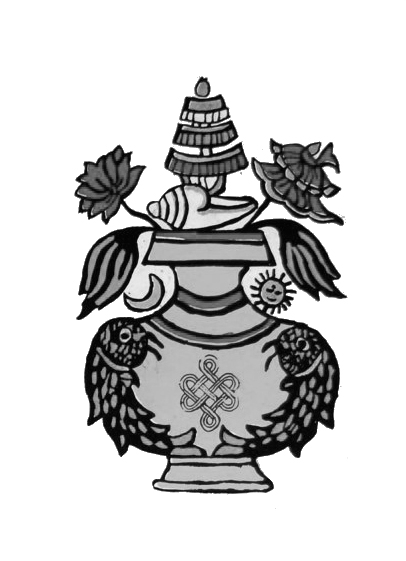
\includegraphics[width=0.25\textwidth]{pics/purna.jpg}
  \end{figure}
  
\newpage

\begin{landscape}
\thispagestyle{empty}
  \begin{figure}[p]
	\centering
  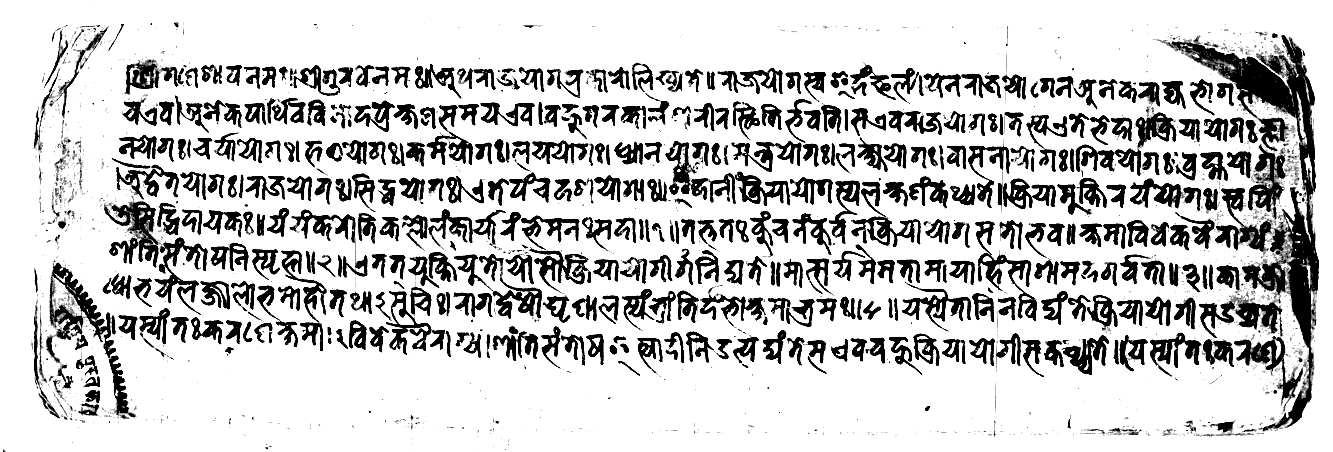
\includegraphics[width=1.5\textwidth]{pics/folio1.jpg}
	\caption{Folio 1v of Ms. \getsiglum{N1}.}
	 \phantomsection\label{fig_folio1}
\end{figure}
\end{landscape}

\cleardoublepage
\tableofcontents
\thispagestyle{empty}
\newpage 
\listoffigures
\thispagestyle{empty}
\newpage
\listoftables
\thispagestyle{empty}
\newpage

\mainmatter
\pagestyle{defaultstyle}
\counterwithout{footnote}{chapter}
\counterwithout{figure}{chapter}
\counterwithout{table}{chapter}
\renewcommand{\thetable}{\arabic{table}}
%%%tables 
\setsecnumdepth{section}
\maxsecnumdepth{subsubsection}
\newpage
\chapter{Introduction}
\cleardoublepage

\section{General remarks}
 \phantomsection\label{generalremarks}
 \lettrine{T}{he} \textit{Tattvayogabindu} of Rāmacandra\footnote{A discussion about the author Rāmacandra is found on p. \pageref{ramarama}.} is an early modern Sanskrit text on Rājayoga that was written in the first half of the seventeenth century\footnote{The dating of the text is discussed on p. \pageref{dating}.} in northern India.\footnote{The detailed discussion of the place of origin is found on p. \pageref{riversrivers}, n. \ref{riversrivers}.} The most salient feature of the work that makes it historically significant is its highly differentiated taxonomy of types of yoga.\footnote{This is a remarkable increase in the number of declared yogas compared to the standard medieval tetrad of Mantra, Laya, Haṭha and Rājayoga.} In the \textit{Tattvayogabindu}'s introduction, most manuscripts name fifteen types of yoga, presented as methods of Rājayoga. These are 1. Kriyāyoga, 2. Jñānayoga, 3. Caryāyoga, 4. Haṭhayoga, 5. Karmayoga, 6. Layayoga, 7. Dhyānayoga, 8. Mantrayoga, 9. Lakṣyayoga, 10. Vāsanāyoga, 11. Śivayoga, 12. Brahmayoga, 13. Advaitayoga, 14. Siddhayoga, and 15. Rājayoga itself. The text is a yogic compendium written in a mix of mainly prose and 47 verses in textbook-style, where its 59 topics are introduced in sections most of the time launched by recognizable phrases. The sections deal with the methods of Rājayoga and their effects, but others also cover topics like yogic physiology, the Avadhūta, the importance of the guru, cosmogony, and a \textit{yogaśāstrarahasya}.  

The \textit{Tattvayogabindu} has not been discussed comprehensively or considered in the secondary literature on yoga. The only exception is \citeauthor{birch2014} (2014: 415–416) who briefly described its list of fifteen yogas in the context of the ``fifteen medieval yogas'' and noted that a similar taxonomy occurs in Nārāyaṇatīrtha’s \textit{Yogasiddhāntacandrikā} (17th century), a commentary on the \textit{Pātañjalayogaśāstra} that integrates fifteen medieval yogas within its \textit{aṣṭāṅga} format. An incomplete account of the fifteen yogas is found within the Sanskrit yoga text \textit{Yogasvarodaya}, which is known only through quotations in the \textit{Prāṇatoṣinī}, the \textit{Yogakarṇikā} and the \emph{Śabdakalpadruma}.\footnote{Manuscripts under the name of \textit{Yogasvarodaya} seem to be lost. I was not able to locate the manuscripts of the text in any manuscript catalogue at hand.} The \textit{Yogasvarodaya} announces a total of fifteen yogas but names only eight of them in its introductory \textit{śloka}s. It is the primary source and template for the compilation of the \textit{Tattvayogabindu}. Besides several passages, Rāmacandra, in many instances, follows its content and structure by rewriting the \textit{Yogasvarodaya}’s \textit{śloka}s into prose or quoting them directly without attribution. Due to the incomplete transmission of the \textit{Yogasvarodaya}, Rāmacandra’s \textit{Tattvayogabindu} is a natural and valuable starting point for an unprecedented in-depth study of the complex early modern yoga taxonomies, a phenomenon that can be narrowed down precisely in terms of time and as I will show regarding its localisation. The other source text that Rāmacandra used is the \textit{Siddhasiddhāntapaddhati} whose content he draws on, particularly in the second half of his composition. Another text that includes an almost similar taxonomy of twelve yogas divided into three tetrads\footnote{See p.\pageref{sarvasarva} for a detailed discussion of the \textit{Sarvāṅgayogapradīpikā}.} is Sundardās’s \textit{Brajbhāṣā} yoga text named \textit{Sarvāṅgayogapradīpikā} which not just shares most of the types of yogas but also provides a different and valuable perspective on the addressed yoga categories.\footnote{For a comparative table of the complex early modern yoga taxonomies see table \ref{tab:complextaxonomies} on p. \pageref{tab:complextaxonomies}.}

These complex taxonomies that emerged during the 17th century crossed sectarian divides and were adapted to the specific needs of different authors and traditions. The \textit{Tattvayogabindu} thus encapsulates a large proportion of the diversity of yoga types and teachings after the \textit{Haṭhapradīpikā} (15th century) that were adopted and practised by a broad spectrum of religious traditions and strata of Indian society. In the particular case of the \textit{Tattvayogabindu}, there are various statements throughout the text that reveal a strategy to detach yoga from its ascetic and renunciate connotations and to stylise Rājayoga as a practice that can bring the desired soteriological benefits even to practitioners who enjoy worldly pleasures and expensive lifestyles. Textual evidence suggests that the \textit{Tattvayogabindu} is an important example of a text that provides an early modern adaptation of Rājayoga for \textit{kṣatriya}s in a courtly environment.

One printed edition of the \textit{Tattvayogabindu} was published in 1905 with a Hindi translation and based on (an) unknown manuscript(s).\footnote{\emph{Binduyoga}. \textit{Binduyogaḥ with Bhāṣaṭīkā}. Ed. by Jvālāprasāda Miśra. Mumbai, 1905.} This publication has the title ``\textit{Binduyoga}'' confirmed by the printed text’s colophon. However, as I will discuss in the introduction, the text was originally known as \textit{Tattvayogabindu}. The consulted manuscripts contain significant discrepancies, structural differences and variant readings between them and the printed edition.\footnote{For example, the printed edition does not contain the complex yoga taxonomy presented in the manuscripts of the \emph{Tattvayogabindu}.} Furthermore, the manuscripts are scattered over the northern half of the Indian subcontinent and Nepal, which suggests that the text was widely transmitted at some point. Lengthy passages of the \textit{Tattvayogabindu} are quoted without attribution in a text called \textit{Yogasaṃgraha} and Sundaradeva’s \textit{Haṭhasaṅketacandrikā}.

The first chapter of this dissertation contains a general introduction to Rāmacandra's \textit{Tattvayogabindu}. The chapter gives a brief overview of the content of the text and discusses its origin, the author and the author's intended audience. Subsequently, the textual witnesses, source texts and testimonies of the \textit{Tattvayogabindu} are described. A stemmatic analysis of the text is then presented, based on manual philological observation and computer-assisted stemmatics to present a \textit{stemma codicum}. The chapter concludes with a presentation of the editorial policies, which form the basis for the second chapter of this thesis.
The second chapter, the core of this dissertation, is a critical edition and annotated translation of the \textit{Tattvayogabindu}. The critical edition significantly improves the text and sheds new light on its historical significance.
The third chapter contains a comparative analysis of the complex early modern yoga taxonomies based on hermeneutics of difference.\footnote{The conceptof hermeneutics of difference is discussed on p. \pageref{hermeneutics}, n. \ref{hemerneutics}.}  Using the new critical edition of the \textit{Tattvayogabindu} and the texts mentioned above, \emph{Yogasvarodaya}, \emph{Yogasiddhāntacandrikā} and \emph{Sarvāṅgayogapradīpikā}, the complex yogic taxonomies of the four texts are compared in detail. Based on this comparative analysis, a differentiated hypothesis on the emergence of the complex yoga taxonomies was developed, and the complex yoga taxonomies were located und explained in the broader context of the historical development of the yoga traditions. The comparison includes a nuanced description of each yoga category used by the authors of the texts with complex yoga taxonomies. While the authors of the four texts often operate with identical terms for the individual yoga categories, they interpret these categories according to their religious backgrounds and agendas, with intriguing and exciting differences. Contrasting the comparanda, i.e. the authors, the texts, the yoga taxonomies and the yoga categories, therefore provides a deep insight into the discursive negotiation processes of the Indian yoga traditions of the 17th century.


\chapter{Conventions in the Critical Apparatus}
\section{Sigla in the Critical Apparatus}

\begin{itemize}
\item \beta : \getsiglum{D}, \getsiglum{J}, \getsiglum{K1}, \getsiglum{N1}, \getsiglum{N2}, \getsiglum{U1}
\item \gamma : \getsiglum{B}, \getsiglum{E}, \getsiglum{L}, \getsiglum{P}, \getsiglum{U2}
\item B : Bodleian Oxford D 4587
\item C : \emph{Haṭhasaṅketacandrikā} GOML Ms. No. R 3239
\item C\textsubscript{pc} : \emph{Haṭhasaṅketacandrikā} GOML Ms. No. R 3239
\item cett.: ceteri (all manuscripts except the ones mentioned in the lemma)
\item \Done : IGNCA 30019
\item E : Printed Edition
\item J : JNUL Ms. No. 55769
\item Jo : \emph{Haṭhasaṅketacandrikā} MMPP MS. No. 2244
\item \Kone : AS G 11019
\item L : Lalchand Research Library LRL5876
\item M : \emph{Haṭhasaṅketacandrikā} ORI Ms. No. B 220
\item \Ntwo : NGMPP B 38-35 / A 1327-14
\item \None : NGMPP B 38-31
\item P : Pune BORI 664
\item PT : \emph{Prāṇatoṣiṇī}
\item \Uone : SORI 1574
\item \Utwo : SORI 6082
\item V : OI MSU 10558
\item YK : \emph{Yogakarṇikā}% 
\item YSv : \emph{Yogasvarodaya}
\end{itemize}
\newpage

\chapter[Critical Edition \& Annotated Translation of the \emph{Tattvayogabindu}]{The \emph{Tattvayogabindu} of Rāmacandra \\ \huge  
  Critical Edition \& Annotated Translation}
\pagestyle{chapter2style}
\newpage
\begin{alignment}[
  texts=edition[class="edition"];
  translation[class="translation"],
  ]
  \begin{edition}
     \ekddiv{
      head={[\uproman{24}. \textbf{antaralakṣyam}]},
      type=section,
      depth=2, 
      n=XXIV
    }
    \xmlhead[h24]{[XXIV. antaralakṣyam]}
    \phantomsection
    \addcontentsline{toc}{section}{XXIV. antaralakṣyam}
\label{antaralaksya}
          \begin{prose}[p24_01]
            \noindent
%-----------------------------
%idānīm anyataraṃ lakṣyaṃ kathyate/ \E
%idānīṃ aṃtaraṃ lakṣyaṃ   kathyate \P
%idānīṃ antaralakṣaṃ      kartavyaṃ// \B
%idānīṃ aṃtaralakṣaṃ      kartavyaṃ// \L
%idānīṃ antaralakṣyakaṃ   kathyate// \N1
%idānīṃ antaralakṣyaṃ     kathyate// \D
%idānīṃ antaraṃ  lakṣyate// \J            
%idānīṃ antaralakṣyaṃ     kathyate// \K1            
%idānīṃ aṇtaralakṣyaṇaṃ   kathyate// \N2
%idānīṃ aṇtaralakṣyaṇaṃ   kathyate \U1
%idānīm ataraṃ lakṣyaṃ    kathyate// \U2
%-----------------------------
%Now the inner target is explained. 
%-----------------------------%_65b
\note[type=source, labelb=_65b, labele=_65e, nosep]{cf. YSv (PT, p. 838): mūlakandotthatalato brahmanāḍīsamudbhavā | śvetavarṇā brahmarandhraparyantam eva tiṣṭhati | eṣā tu brahmarandhrākhyā tanmadhye varttate parā | padmatantusamākārā koṭisūryataḍitprabhā | calaty ūrddhaṃ mahāmūrttir asya dhyānād bhavec chivaḥ | aṇimādy aṣṭasiddhis tu samagreṇa prasīdati |}         
\note[type=source, labelb=_65b, labele=_65e, nosep]{cf. SSP 2.26 (Ed. pp. 37-38): tatra tāvad antarlakṣyaṃ kathyate | mūlakandād daṇḍalagnāṃ brahmanāḍīṃ śvetavarṇāṃ brahmarandhraparyantaṃ gatāṃ saṃsmaret | tanmadhye kamalatantunibhāṃ vidyutkoṭiprabhām ūrdhvagāminīṃ tāṃ mūrtiṃ manasā lakṣayet | sarvasiddhipradā bhavati |}            
\note[type=testium, labelb=_65b, labele=_65e, nosep]{ \approx  \citetitle{hathasamketacandrikajodhpur} (MMPP 2244 f. 125r ll. 8-9 - f. 126v l. 1): athāṃtarlakṣyaṃ nirūpyate | mūlakaṃdasthāne brahmadaṃḍād utpannāśvetavarṇābrahmaraṃdhraparyaṃttaṃ ekābrahmanāḍī vartate | brahmanāḍī madhye kamalataṃtusamānākārakoṭisūryavidyutprabhā tulyā ūrdhva calati | etādṛśī ekā mūrtir vartate | tasya mūrter dhyānakaraṇād aṇimādisiddhayaḥ samīpa upatiṣṭhaṃte |}    
\app{\lem[wit={E,U2},alt={idānīm}]{idānī\skp{m-a}}\linelabel{_65b}
  \rdg[wit={ceteri}]{idānīṃ}   
}\app{\lem[wit={D,K1}, alt={antaralakṣyaṃ}]{\skm{m-a}ntaralakṣyaṃ}
  \rdg[wit={E}]{anyataraṃ lakṣyaṃ}
  \rdg[wit={P}]{aṃtaraṃ lakṣyaṃ}
  \rdg[wit={B,L}]{antaralakṣaṃ}
  \rdg[wit={N1}]{antaralakṣyakaṃ}
  \rdg[wit={N2,U1}]{aṇtaralakṣyaṇaṃ}
  \rdg[wit={U2}]{ataraṃ lakṣyaṃ}
  \rdg[wit={J}]{antaraṃ}}
\app{\lem[wit={ceteri}]{kathyate}
  \rdg[wit={B,L}]{kartavyaṃ}
  \rdg[wit={J}]{lakṣyate}}/    
%-----------------------------
%mūlakandasthāne brahmadaṇḍotpannā nāḍī śvetavarṇā   brahmadaṇḍaparyantam   ekā brahmanāḍī varttate/ \E
%mūlakaṃdasthāne brahmānaṃḍād utpannā   śvetavarṇā   brahmaraṃdhraparyaṃtaṃ ekā brahmanāḍī varttate   \P
%mūlakaṃ sthāne  brahmānaṃḍād utpannā   śvetāvarṇā   brahmaraṃdhraparyaṃtaṃ ekā nāḍī       vartate/     \B
%mūlakaṃdasthāne brahmānaṃdād utpannā   śvetāvarṇā   brahmaraṃdhraparyaṃtaṃ ekanāḍī        vartate/     \L
%mūlakaṃdasthāne brahmadaṃḍa ityannā    śvetavarṇā   brahmaraṃdhraparyaṃtaṃ ekā brahmanāḍī varttate/ \N1
%mūlakaṃdasthāne brahmadaṃḍād utpannā   śvetavarṇā// brahmaraṃdhraparyaṃtaṃ ekā brahmanāḍī varttate// \D
%mūlakaṃdasthāne brahmadaṃḍād utpannā   śvetavarṇaṃ// brahmaraṃdhraparyaṃtaṃ ekā brahmanāḍī varttate// \K1
%mūlakaṃdasthāne brahmadaṃḍād utpannāḥ  śvetavarṇaṃ// brahmaraṃdhraparyaṃtaṃ ekā brahmanāḍī varttate// \J (P14/34)
%mūlakaṃdasthāne brahmadaṇḍad ūtpannā   śvetavarṇā   brahmaraṃdhraparyaṃtaṃ ekā brahmanāḍī varttate/ \N2
%mūlakaṃdasthāne brahmadaṇād ūtpannaḥ   śvetavarṇāṃ  brahmaraṃdhraparyaṃtaṃ ekā brahmanāḍī varttate \U1
%mūlakaṃdasthāne brahmadaṇḍād utpannā   śvetavarṇā   brahmaraṃdhraparyaṃtaṃ ekā brahmanāḍī varttate// \U2
%-----------------------------
%Starting from the location of the root-bulp (\textit{mūlakanda}) originating from the staff of Brahma, being white in colour, extending up to the aperture of Brahma [at the top the head] exists the single Brahma-channel.
%-----------------------------
\app{\lem[wit={ceteri}]{mūlakandasthāne}
  \rdg[wit={P}]{mūlakaṃ sthāne}}
brahma\app{\lem[wit={ceteri}, alt={°daṇḍād utpannā}]{daṇḍād\skp{-}utpannā}
  \rdg[wit={E}]{brahmadaṇḍotpannā nāḍī}
  \rdg[wit={N1}]{brahmadaṃḍa ityannā}
  \rdg[wit={N2}]{brahmadaṇḍad ūtpannā}
  \rdg[wit={K1}]{daṃḍād utpannāḥ}
  \rdg[wit={U1}]{brahmadaṇād ūtpannaḥ}}
śveta\app{\lem[wit={ceteri}, alt={°varṇā}]{varṇā}
  \rdg[wit={U1}]{°varṇāṃ}
   \rdg[wit={J,K1}]{°varṇaṃ}}
brahma\app{\lem[wit={ceteri}, alt={°randhraparyaṃtaṃ}]{randhra:\\paryaṃtaṃ}
  \rdg[wit={E}]{°daṇḍaparyantam}} 
\app{\lem[wit={ceteri}, alt={ekā brahmanāḍī}]{ekā brahmanāḍī}
  \rdg[wit={B}]{ekā nāḍī}
  \rdg[wit={L}]{ekanāḍī}}
vartate/
%-----------------------------
%brahmanāḍīmadhye kamalatantusamānākārā koṭisūryavidyutsamaprabhā   ūrdhvaṃ calati/  \E
%brahmanāḍīmadhye kamalataṃ samānākārā  koṭisūryavidyutsamaprabhā   ūrdhvaṃ calati   \P
%brahmanāḍīmadhye kamalataṃtusamānākārā koṭisūryavidyutsabhāprabhā  ūrdhvaṃ calati/  \B
%brahmanāḍīmadhye kamalataṃtusamānākārā koṭisūryavidyutsabhāprabhā  ūrdhvaṃ calati/  \L
%brahmanāḍīmadhye kamalatantusamānākārā koṭisūryavidyutsamaprabhā   ūrdhvaṃ calati/  \N1
%brahmanāḍīmadhye kamalataṃtusamānākārā koṭisūryavidyutsamaprabhā   ūrdhvaṃ calati// \D
%brahmanāḍīmadhye kamalataṃtusamānākārā koṭisūryavidyutsamaprabhā   ūrdhvaṃ calati \J
%brahmanāḍīmadhye kamalataṃtusamānākārā koṭisūryavidyutsamaprabhā   ūrdhvaṃ calati// \K1
%\om                                                                                 \N2
%brahmanāḍīmadhye kamalatantusamānākārā koṭisūryavidyutsamaprabhā    rdhvaṃ ccalati  \U1
%brahmanāḍīmadhye kamalataṃtusamānākārā koṭisūryavidyutsamaprabhā// urdhvaṃ calati   \U2 %%%412.jpg 
%-----------------------------
%Within the Brahma channel [exists something] resembling the shape of a stalk of a lotus-flower shining like 10 million suns [which] goes upwards. 
%-----------------------------
\app{\lem[wit={ceteri}]{brahmanāḍī madhye}
  \rdg[wit={N2}]{\om}} 
\app{\lem[wit={ceteri}]{kamalatantusamānākārā}
  \rdg[wit={P}]{kamalataṃ samānākārā}
  \rdg[wit={N2}]{\om}}
koṭisūrya:\\vidyut\app{\lem[wit={ceteri}, alt={°samaprabhā}]{samaprabhā}
  \rdg[wit={B,L}]{°sabhāprabhā}
  \rdg[wit={N2}]{\om}}
\app{\lem[wit={ceteri}]{ūrdhvaṃ}
  \rdg[wit={U1}]{°rdhvaṃ}
  \rdg[wit={U2}]{urdhvaṃ}
\rdg[wit={N2}]{\om}}
\app{\lem[wit={ceteri}]{calati}
  \rdg[wit={N2}]{\om}}/
%-----------------------------
%etādṛśy ekā mūrttir varttate/  tan    mūrter dhyānakāraṇāt      aṣṭamahāsiddhayo  'ṇimādayas   tasya                                                                                puruṣasya samīpam āgatya tiṣṭhanti// \E
%etādṛśy ekā mūrttir vartate    tasyā  mūrter dhyānakaraṇāt      aṣṭamahāsiddhayo   ṇimādyāḥ    aṇimā-mahimā-laghīmā-girimā-dure dīya vā            dure  stutvā parakāyapraveśītā   puruṣasya samīm   āgatya tiṣṭhaṃti \P
%etādṛśy ekā mūrttir varttate/  tasyā  mūrte  dhyānakaraṇāt//    aṣṭamahāsiddhayo// aṇimādyāḥ// aṇimā-mahimā-laghimā-girimā-dure vā yadi vā yadi vā dure  śrutvā parakāyāpraveśitā// puruṣasya samīpem āgatya tiṣṭhati// \B
%etādṛśy ekā mūrttir varttate/  tasyā  mūrter dhyānakaraṇāt//    aṣṭamahāsiddhayo   aṇimādyāḥ// aṇimā-mahimā-laghimā-garimā-dure vā yadi         vā ddure śrutvā parakāyāpraveśitā   puruṣasya samīpam āgatya tiṣṭhati// \L
%etādṛśī ekā mūrttir varttate/  tasyāḥ mūrtter dhyānakāraṇāt/    aṇimādīsiddhiḥ                                                                                                      puruṣasya samīpe? āgatya tiṣṭhanti// \N1
%etādṛśī ekā mūrttir varttate// tasyā  mūrtter dhyānakāraṇāt//   aṇimādyaṣṭasiddhiḥ                                                                                                  puruṣasya samīpe  āgatya tiṣṭhati// \D
%etādṛśī ekā mūrttir varttate// tasyā  mūrtter dhyānakāraṇāt//   aṇimādyaṣṭasiddhiḥ                                                                                                  puruṣasya samīpe  āgatya tiṣṭhati// \K1
%etādṛśī ekā mūrttir varttate// tasyā  mūrtter dhyānakāraṇāt//   aṇimādyaṣṭasiddhiḥ puruṣasya samīpe  āgatya tiṣṭhati// \J
%\om                            tasyā  mūrtter dhyānakaraṇāc                                                                                                                                                            \N2
%                                                                aṇimādyaṣṭasiddhiḥ                                                                                                  puruṣasya sāmīpe  āgatya tiṣṭhati \U1
%etādṛśy ekā mūrttir varttate// tasyā   mūrter dhyānakaraṇāt//   aṣṭamahāsiddhayo aṇimādyāḥ//                                                                                        puruṣasya samīpam āgamya tiṣṭhati// \U2
%-----------------------------
%[There] exists only one such manifestation. Due to the execution of meditation on this manifestation, the eight great supernatural powers of humans beginning with "becoming as small as the smallest particle of matter" (\textit{aṇima}) etc. become established after one has entered into [the manufestation's] imminence. 
%-----------------------------
\app{\lem[wit={ceteri}, alt={etādṛśy ekā°}]{etādṛ\skp{śy-e}}
  \rdg[wit={D,J,K1,N1}]{etādṛśī}
  \rdg[wit={U1,N2}]{\om}}\skm{śy-e}kā
\app{\lem[wit={ceteri}, alt={mūrtir}]{mūrti\skp{r-va}}
  \rdg[wit={U1,N2}]{\om}
}\app{\lem[wit={ceteri}, alt={vartate}]{\skm{r-va}rtate}
  \rdg[wit={U1,N2}]{\om}}/
\app{\lem[wit={ceteri}, alt={tasyā}]{tasyā}
  \rdg[wit={N1}]{tasyāḥ}
  \rdg[wit={E}]{tan}
  \rdg[wit={U1}]{\om}}
\app{\lem[wit={ceteri}, alt={mūrter}]{mūrte\skp{r-dhyā}}
  \rdg[wit={B}]{mūrte}
  \rdg[wit={U1}]{\om}
}\app{\lem[wit={ceteri}, alt={dhyāna°}]{\skm{r-dhyā}na}
  \rdg[wit={U1}]{\om}
}\app{\lem[resp=egoscr, type=emendation, alt={°kāraṇād}]{kāraṇā:\\\skp{d-a}}
  \rdg[wit={ceteri}]{°karaṇāt}
  \rdg[wit={N2}]{°karaṇāc°}
  \rdg[wit={U1}]{\om}
}\app{\lem[wit={D,J,K1,U1}, alt={aṇimādyaṣṭasiddhiḥ}]{\skm{d-a}ṇimādyaṣṭasiddhiḥ}
  \rdg[wit={N1}]{aṇimādīsiddhiḥ}
  \rdg[wit={U2}]{aṣṭamahāsiddhayo aṇimādyāḥ ||}
  \rdg[wit={E}]{aṣṭamahāsiddhayo 'ṇimādayas tasya}
  \rdg[wit={B}]{aṣṭamahāsiddhayo || aṇimādyāḥ || aṇimāmahimālaghimāgirimā dure vā yadi vā yadi vā dure śrutvā parakāyāpraveśitā ||}
  \rdg[wit={L}]{aṣṭamahāsiddhayo aṇimādyāḥ || aṇimāmahimālaghimāgarimā dure vā yadi vā ddure śrutvā parakāyāpraveśitā}
  \rdg[wit={P}]{aṣṭamahāsiddhayo ṇimādyāḥ aṇimāmahimālaghīmāgirimādure dīya vā dure stutvā parakāyapraveśītā}}
\app{\lem[wit={ceteri}]{puruṣasya}
  \rdg[wit={N2}]{\om}} 
\app{\lem[wit={D,J,K1,N1}]{samīpe}
  \rdg[wit={U1}]{sāmīpe}
  \rdg[wit={B}]{samīpem}
  \rdg[wit={E,L,U2}]{samīpam}
  \rdg[wit={P}]{samīm}
\rdg[wit={N2}]{\om}}
\app{\lem[wit={ceteri}]{āgatya}
  \rdg[wit={U2}]{āgamya}
\rdg[wit={N2}]{\om}}
\app{\lem[wit={ceteri}]{tiṣṭhati}
  \rdg[wit={E,P,N1}]{tiṣṭhanti}
  \rdg[wit={N2}]{\om}}/\linelabel{_65e}
\end{prose}
\end{edition}
\begin{translation}
    \ekddiv{
      head={[\uproman{24}. \textbf{The inner focus}]},
      type=section,
      depth=2, 
      n=XXIV.1a
    }
    \xmlhead[h25]{[XXIV. Antaralakṣya]}
\begin{tlate}[p24_01]
\noindent
Now, the inner focus is explained. At the location of the root-bulb (\textit{mūlakanda})\footnote{Various concepts of the location of the \textit{kanda} exist in yogic literature. In the \citetitle{yajnavalkya} 4.16-27 one reads: \textit{kandasthānāṃ manuṣyāṇāṃ dehamadhyān navāṅgulam} | \textit{caturaṅgulam utsedham āyāmaś ca tathāvidhaḥ} || 16 || \textit{aṇḍākṛtivad ākāraṃ bhūṣitaṃ tattvagādhibhiḥ} | \textit{catuṣpadāṃ tiraścāṃ ca dvijānāṃ tundamadhyame} || 17 || ``The location of the bulb (\textit{kanda}) of humans is nine finger widths from the waist. [It is] four finger widths in height and has the same [measure in] length. It appears like an egg, and [it is] ornamented with the five elements of creation and sustenance. In quadrupeds, birds and other beings, it is in the centre of the belly.'' \citetitle{hathapradipika2024} 3.64cd (\textit{gulphadeśasamīpe ca kandaṃ tatra prapīḍayet}) instructs the yogin to press the \emph{kanda} with the feet in the context of \textit{uḍḍiyāṇabandha}, which could imply that the \emph{kanda} is in the genital region (unless one assumes the very complex and challenging posture termed \textit{kandapīḍāsana}, cf. \citetitle{encyclopediaasana}, pp. 143-144). Sundaradeva, in \citetitle{yuktabhavadeva} 7.224 and Bhavadevamiśra in \citetitle{hathasamketacandrikajodhpur} (MMPP Ms. No. 2244, f. 36r) argue that the \emph{kanda} is near the navel. In \citetitle{yogacudamani} 14cd the \textit{kanda} is in between penis and navel (\textit{ūrdhvaṃ meḍhrādadho nābheḥ kande yoniḥ khagāṇḍavat}).} originating from the staff of Brahman,\footnote{The term \textit{brahmadaṇḍa} in this context refers to the spinal column, which is usually identified with Mt. Meru in tantric texts, cf. \citeauthor[1988: 360]{stupa}.} being white, extending up to the aperture of Brahman exists the single Brahman-channel.\footnote{The term \textit{brahmanāḍī} is a synonym for the \textit{suṣūmnā}, cf., e.g. \citetitle{hathapradipika2024} 2.67, \emph{Gorakṣaśataka}\nocite{mallinson2012sataka} 47, \citetitle{yogakundalinyopanisad} 37c-38b, \citetitle{yogacintamani} (Ed. pp. 46, 112, 116, 140, 191), \citetitle{hatharatnavali} 2.8, 2.25, 2.65, 2.69.} The Brahman-channel, being within [the staff of Brahman],\footnote{Naturally, one would read \textit{brahmanāḍīmadhye} compounded, but this would leave the sentence lacking a subject. Therefore, the only option is to read \textit{brahmanāḍī madhye} separately, referring to the inside of the previously mentioned \textit{brahmadaṇḍa}. Assuming another channel within the \textit{brahmanāḍī} like the \textit{citrānāḍī} in \citetitle{mallinson2007} 5.160 would be difficult to proof.} having the shape of a stalk of a lotus flower [and] shining like ten million suns goes upwards. One such manifestation exists. As a result of meditation on this manifestation\footnote{Cf. \citetitle{bäumer2013} 35.} %: `The central channel, which is situated within the centre of the body [is endowed] with a form resembling the stalk of a lotus. By meditation upon its empty inner space, god becomes revealed by the goddess [of the middle].' (\textit{madhyanāḍī madhyasaṃsthā bisasūtrābharūpayā} | \textit{dhyātāntarvyomayā devyā tayā devaḥ prakāśate} |)},
the accomplishment of the eight supernatural powers beginning with `becoming as small as the smallest particle of matter' etc.\footnote{For a detailed discussion of the yogic \textit{siddhi}s, see \citeauthor[2017]{yogapowers2017}.} exists in proximity of the person.\begin{buber}[f24_1]\footnote{Three of five witnesses of the \gamma-group add an incomplete list of the eight \textit{siddhi}s \ldots}\end{buber} 
%\flushpage
    \end{tlate}
  \end{translation}
\end{alignment}
\pagebreak %after pp. 77-78
%%%%%%%%%%%%%%%%%%%%%%%%%%%%%%%%%%%%%%%%%%
%%%%%%%%%%%%%%%%%%%%%%%%%%%%%%%%%%%%%%%%%% 
%%%%%%%%PAGEBREAK%%%%%%%PAGEBREAK%%%%%%%%%
%%%%%%%%%%%%%%%%%%%%%%%%%%%%%%%%%%%%%%%%%% 
%%%%%%%%%%%%%%%%PAGEBREAK%%%%%%%%%%%%%%%%%
%%%%%%%%%%%%%%%%%%%%%%%%%%%%%%%%%%%%%%%%%% 
%%%%%%%%PAGEBREAK%%%%%%%PAGEBREAK%%%%%%%%%
%%%%%%%%%%%%%%%%%%%%%%%%%%%%%%%%%%%%%%%%%% 
%%%%%%%%%%%%%%%%%%%%%%%%%%%%%%%%%%%%%%%%%% 
%%%%%%%%%%%%%%%%%%%%%%%%%%%%%%%%%%%%%%%%%% 
%%%%%%%%%%%%%%%%%%%%%%%%%%%%%%%%%%%%%%%%%% 
%%%%%%%%PAGEBREAK%%%%%%%PAGEBREAK%%%%%%%%%
%%%%%%%%%%%%%%%%%%%%%%%%%%%%%%%%%%%%%%%%%% 
%%%%%%%%%%%%%%%%PAGEBREAK%%%%%%%%%%%%%%%%%
%%%%%%%%%%%%%%%%%%%%%%%%%%%%%%%%%%%%%%%%%% 
%%%%%%%%PAGEBREAK%%%%%%%PAGEBREAK%%%%%%%%%
%%%%%%%%%%%%%%%%%%%%%%%%%%%%%%%%%%%%%%%%%% 
%%%%%%%%%%%%%%%%%%%%%%%%%%%%%%%%%%%%%%%%%% 
%%%%%%%%%%%%%%%%%%%%%%%%%%%%%%%%%%%%%%%%%% 
%%%%%%%%%%%%%%%%%%%%%%%%%%%%%%%%%%%%%%%%%% 
%%%%%%%%PAGEBREAK%%%%%%%PAGEBREAK%%%%%%%%%
%%%%%%%%%%%%%%%%%%%%%%%%%%%%%%%%%%%%%%%%%% 
%%%%%%%%%%%%%%%%PAGEBREAK%%%%%%%%%%%%%%%%%
%%%%%%%%%%%%%%%%%%%%%%%%%%%%%%%%%%%%%%%%%% 
%%%%%%%%PAGEBREAK%%%%%%%PAGEBREAK%%%%%%%%%
%%%%%%%%%%%%%%%%%%%%%%%%%%%%%%%%%%%%%%%%%% 
%%%%%%%%%%%%%%%%%%%%%%%%%%%%%%%%%%%%%%%%%%
\begin{alignment}[
  texts=edition[class="edition"];
  translation[class="translation"],
  ]
  \begin{edition}
    \begin{prose}[p24_02]
\noindent
%-----------------------------
%athavā lalāṭopary ākāśamadhye śuklasadṛśasya tejaso dhyānakāraṇāt       śarīrasambandhinaḥ  kuṣṭhādayo rogā  naśyanti/    āyur vṛddhir bhavati/  \E
%athavā lalāṭopari ākāśamadhye śuklasadṛśasya tejaso dhyānakāraṇāt       śarīrasaṃbaṃdhinaḥ  kuṣṭhādayo rogāḥ naśyaṃtī     āyur vṛddhir bhavati   \P  %%%7647.jpg
%athavā lalāṭopari ākāśamadhye śuklasadṛśasya tejaso dhyānakāraṇāt//     charīrasambandhinaḥ kuṣṭhādayo rogā  naśyaṃtī//   āyur vṛddhir bhavatī   \B 
%athavā lalāṭopari ākāśamadhye śuklasadṛśasya tejaso dhyānakāraṇāt       charīrasambandhinaḥ kuṣṭhādayo rogā  naśyaṃti//   āyur vṛddhir bhavati// \L
%athavā lalāṭopari ākāśamadhye śuklasadṛśasya tejaso dhyānakāraṇāt       śarīrasambandhī     kuṣṭhādayo rogāḥ naśyaṃti/    āyur vṛddhir bhavati/  \N1
%athavā lalāṭopari ākāśamadhye śuklasadṛśasya tejaso dhyānakāraṇāt       śarīrasaṃbaṃdhī     kuṣṭādayo  rogāḥ naśyaṃti//   āyur vṛddhir bhavati//  \D
%athavā lalāṭopari ākāśamadhye śuklasadṛśasya tejaso dhyānakāraṇāt       śarīrasaṃbaṃdhī     kuṣṭādayo  rogāḥ naśyaṃti//   āyur vṛddhir bhavati//  \K1
%athavā lalāṭopari ākāśamadhye śuklasadṛśasya tejaso dhyānakāraṇāt//       śarīrasaṃbaṃdhī     kuṣṭādayo  rogāḥ naśyaṃti//   āyur vṛddhir bhavati//cha//  \J      
%                                                                         charīrasaṃbaṃdhi----kuṣṭadayo  rogāḥ naśyaṃti     āyur vṛddi   bhavati/  \N2
%atha vā lalāṭoparī ākāśamadhye śuklasadṛśasya tejo   dhyānakāraṇāt       śarīrasambaṃdhī     kuṣṭhādayo rogā  naśyaṃti     āyur vṛddhir bhavati   \U1 %%%279.jpg
%atha vā lalāṭoparī ākāśamadhye śuklasadṛśasya tejaso dhyānakāraṇāt//     śarīrasambaṃdhinaḥ  kuṣṭhādayo rogā  naśyaṃti//   āyur vṛddhir bhavati//  \U2
%-----------------------------
%Or from the execution of meditation onto the bright light at the centre within the space above the forehead diseases related to the body beginning with leprosy vanish. Lifeforce increases.   
%-----------------------------
\note[type=source, labelb=_66b, labele=_66e, nosep]{cf. YSv (PT, p. 838): lalāṭopari vā dhyātvā candraṃ vā jyotir īśvaram | nāśayet kuṣṭharogādīn mahāyuṣmān śivaḥ paraḥ | bhruvor madhye 'thavā dhyātvā arkantu teja īśvaram | sthiradṛṣṭau rājapūjyo jīvanmuktaḥ śivo yathā | ātmānam ātmarūpaṃ hi dhyātvā yo niṣkriyo bhavet | nirāśīryatatattvo 'yaṃ itaro na nṛpasthitiḥ |}
\note[type=source, labelb=_66b, labele=_66e, nosep ]{cf. SSP 2.27 (Ed. p. 38): athavā lalāṭordhve gollāṭamaṇḍape sphurattārākāraṃ lakṣayet |}
\note[type=testium, labelb=_66b, labele=_66e, nosep]{ \approx  \citetitle{hathasamketacandrikajodhpur} (MMPP 2244 f. 125v ll. 1-3): athāvā lalāṭopari ākāśamadhye śukladṛśyasya tejaso dhyānakaraṇāc charīrāḥ kuṣṭḥādiroga naśyaṃtīti | athavā bhruvor madhye atiraktavarṇasyātisthūlasya tejaso dhyānakaraṇāt kalānāṃ pārthivapuruṣāṇāṃ vallabho bhavati | taṃ puruṣaṃ dṛṣṭvā sarveṣāṃ puruṣāṇāṃ dṛṣṭiḥ sthirā bhavatī |}
athavā\linelabel{_66b}
\app{\lem[wit={E}, alt={lalāṭopary}]{lalāṭopa\skp{ry-ā}}
  \rdg[wit={B,D,J,K1,L,N1}]{lalāṭopari}
  \rdg[wit={U1,U2}]{lalāṭoparī}
  \rdg[wit={N2}]{\om}
}\app{\lem[wit={ceteri}, alt={ākāśamadhye}]{\skm{ry-ā}kāśamadhye}
  \rdg[wit={N2}]{\om}}
\app{\lem[wit={ceteri}]{śuklasadṛśasya}
  \rdg[wit={N2}]{\om}} 
\app{\lem[wit={ceteri}]{tejaso}
  \rdg[wit={N2}]{\om}} 
\app{\lem[resp=egoscr, type=emendation, alt={dhyānakaraṇāc}]{dhyānakāraṇā\skp{c-cha}}
  \rdg[wit={ceteri}]{dhyānakāraṇāt}
  \rdg[wit={N2}]{\om}
}\app{\lem[wit={B,L}, alt={śarīra°}]{\skm{c-cha}rīra}
  \rdg[wit={ceteri}]{śarīra°}
  \rdg[wit={N2}]{\om}
}\app{\lem[wit={Y}, alt={°sambandhinaḥ}]{sambandhi:\\naḥ}
  \rdg[wit={D,J,K1,N1,U1}]{°sambandhī}
  \rdg[wit={N2}]{°saṃbaṃdhi}}
\app{\lem[wit={ceteri}]{kuṣṭhādayo}
  \rdg[wit={D,J,K1,N2}]{kuṣṭādayo}}
\app{\lem[wit={ceteri}]{rogā}
  \rdg[wit={D,J,K1,P,N1,N2}]{rogāḥ}}
\app{\lem[wit={ceteri}, alt={naśyanti}]{naśyanti}
  \rdg[wit={B,P}]{naśyaṃtī}}/
āyu\skp{r-vṛ}\app{\lem[wit={ceteri}, alt={vṛddhir}]{\skm{r-vṛ}ddhi\skp{r-bha}}
  \rdg[wit={N2}]{vṛddi}}\app{\lem[wit={ceteri}, alt={bhavati}]{\skm{r-bha}vati}
  \rdg[wit={J}]{bhavati || cha ||}}/ 
%-----------------------------
%          bhruvor madhye  tiriktavarṇasyātisthūlasya     tejaso dhyānakāraṇād bahulānāṃ   pārthivānāṃ tatpuruṣāṇāṃ ca vallabho bhavati/ jagadvallabho pi bhavati/      \E
%atha vā   bhruvor madhye  tiraktavarṇasyātisthūlasya     tejaso dhyānakaraṇāt   sakalānāṃ pārthivapuruṣāṇāṃ           vallabho bhavati          \P
%atha vā// bhruvor madhye 'tiraktavarṇasyātisthūlasya     tejaso dhyānaṃ karaṇāt-sakalānāṃ pārthivapuruṣāṇāṃ vallabho bhavati/         \B DSCN7163.jpg Z.1
%atha vā// bhruvor madhye 'tiraktavarṇasyātisthūlasya     tejaso dhyānakaraṇāt   sakalānāṃ pārthivapuruṣāṇāṃ vallabho bhavati/         \L
%atha vā   bhruvor madhye 'tiraktavarṇasyātisthūlasya     tejaso dhyānakaraṇāt-sakalānāṃ   pārthivapuruṣāṇāṃ vallabho bhavati/           \N1
%atha vā   bhruvor madhye 'tiraktavarṇasyātisthūlasya     tejaso dhyānakaraṇāt-sakalānā    pārthivapuruṣāṇāṃ vallabho bhavati             \D %%%p.10 verso
%atha vā   bhruvor madhye 'tiraktavarṇasyātisthūlasya     tejaso dhyānakaraṇāt-sakalānā    pārthivapuruṣāṇāṃ vallabho bhavati             \K1
%atha vā bhruvor madhye    tiraktavarṇasyātisthūlasya//     tejaso dhyānakaraṇāt-sakalānāṃ    pārthivapuruṣāṇāṃ vallabho bhavati//             \J 
%atha vā   bhruvor madhye  tiraktavarṇasyātisthūlasya     tejaso dhyānakaraṇāt-sakālānāṃ   pārthivapuruṣāṇāṃ vallabho bhavati/             \N2
%atha vā   bhruvor madhye  tiraktavarṇasyātī sthalasya    tejaso dhyānakaraṇāt sakalānāṃ   pārthivapuruṣāṇāṃ vallabho bhavati/          \U1
%atha vā   bṛvor   madhye atiraktavarṇasya 'tisthūlasyaḥ  tejāso dhyānakaraṇāt sakalānāṃ   pārthivapuruṣāṇāṃ vallabho bhavati         \U2
%-----------------------------
%Or because of executing meditation on the very subtle and red coloured light in the middle of the eyebrows, he becomes one who is beloved among all royal people.    
%-----------------------------
\app{\lem[wit={ceteri}]{athavā}
  \rdg[wit={E}]{\om}}
\app{\lem[wit={ceteri}, alt={bhruvor}]{bhruvo\skp{r-ma}}
  \rdg[wit={U2}]{bṛvor}
}\skm{r-ma}dhye\app{\lem[wit={ceteri}, alt={'tirakta°}]{'tirakta}
  \rdg[wit={U2}]{atirakta°}
  \rdg[wit={E}]{tirikta°}
}\app{\lem[wit={ceteri}, alt={varṇasyātisthūlasya}]{varṇasyā:\\tisthūlasya}
  \rdg[wit={U1}]{varṇasyātī sthalasya}
  \rdg[wit={U2}]{'tisthūlasyaḥ}}
tejaso
\app{\lem[wit={ceteri}, alt={dhyānakaraṇāt}]{dhyānakaraṇā\skp{t-sa}}
  \rdg[wit={B}]{dhyānaṃ karaṇāt}
  \rdg[wit={E}]{dhyānakāraṇād}
}\app{\lem[wit={B,L,N1,P,U1,U2},alt={sakalānāṃ}]{\skm{t-sa}kalānāṃ}
  \rdg[wit={N2}]{sakālānāṃ}
  \rdg[wit={D,K1}]{sakalānā}
  \rdg[wit={E}]{bahulānāṃ}}
\app{\lem[wit={ceteri}, alt={pārthivapuruṣāṇāṃ}]{pārthivapuruṣāṇāṃ}\phantomsection\label{royalpeople}
  \rdg[wit={E}]{parthivānāṃ tatpuruṣāṇāṃ ca}}
vallabho
\app{\lem[wit={ceteri}]{bhavati}
  \rdg[wit={E}]{bhavati | jagad vallabho pi bhavati}}/
%-----------------------------
%asya puruṣasyāvalokanena sarveṣāṃ dṛṣṭiḥ sthirā bhavati// \E
%taṃ  puruṣaṃ        pratisarveṣāṃ dṛṣṭiḥ sthirā bhavati  \P
%taṃ  puruṣaṃ        pratisarveṣāṃ dṛṣṭisthirā bhavatī// \B
%taṃ  puruṣa         pratisarveṣāṃ dṛṣṭisthirā bhavati// \L
%taṃ  puruṣaṃ dṛṣṭvā      sarveṣāṃ dṛṣṭisthirā bhavati// \N1
%taṃ  puruṣaṃ dṛṣṭvā      sarveṣāṃ dṛṣṭisthirā bhavati// \D
%taṃ  puruṣaṃ dṛṣṭvā      sarveṣāṃ dṛṣṭisthirā bhavati// \K1
%taṃ  puruṣaṃ dṛṣṭvā      sarveṣāṃ dṛṣṭiḥ sthirā bhavati//cha// \J
%taṃ  puruṣaṃ dṛṣṭā       sarveṣāṃ dṛṣṭisthirā bhavati// \N2
%taṃ  puruṣaṃ dṛṣṭvā      sarveṣāṃ dṛṣṭisthirā bhavati \U1
%taṃ  puruṣaṃ        pratisarveṣāṃ dṛṣṭisthirā bhavati// \U2
%----------------------------
%Having seen this person, everybody's gaze becomes fixed [onto the person]. 
%-----------------------------
\app{\lem[wit={ceteri}]{taṃ}
  \rdg[wit={E}]{asya}}
\app{\lem[wit={D,J,N1,U1}]{puruṣaṃ dṛṣṭvā}
  \rdg[wit={N2}]{puruṣaṃ dṛṣṭā}
  \rdg[wit={B,P}]{puruṣaṃ}
  \rdg[wit={L}]{puruṣa°}
  \rdg[wit={E}]{puruṣasyāvalokanena}}
\app{\lem[wit={X,E}]{sarveṣāṃ}
  \rdg[wit={ceteri}]{pratisarveṣāṃ}}
\app{\lem[wit={E,J,P}]{dṛṣṭiḥ sthirā}
  \rdg[wit={ceteri}]{dṛṣṭisthirā}}
\app{\lem[wit={ceteri}]{bhavati}
  \rdg[wit={B}]{bhavatī}
  \rdg[wit={J}]{bhavati || cha ||}}\dd{}\linelabel{_66e}
    \end{prose}
  \end{edition}
  \begin{translation}
    \begin{tlate}[p24_02]
\begin{euber}[f24_1]\blfootnote{\hspace{-2.2em} (see apparatus). I did not include it in greyscale for two reasons. First, the passage is incomplete and in a very corrupt state. Second, since it is absent \getsiglum{U2} it probably does not belong to the \gamma-group archetype. The passage \textit{dure vā yadi vādure śrutvā} seems to refer to the supernatural abilities \textit{dūradarśana} and \textit{dūraśravana}. The list does not follow the standard list of eight supernatural powers. After the first four items that are usually considered as primary \textit{siddhi}s, the three manuscripts instead list three of the so-called secondary \textit{siddhi}s, cf. \citetitle{bhagavata} 11.10 and 11.15.2-6. Because of that, it is impossible to determine the missing \textit{siddhi} precisely. However, the passage allows to identify seven \textit{siddhi}s: Aṇimā (``the ability to reduce size to the size of the smallest particle''), Mahimā (``the ability to expand one's body to an infinitely large size''), Laghimā (``the ability to become weightless or lighter than air''), Garimā (``the ability to become heavy or dense''), Dūraśravaṇa (``hearing things far away''), Dūradarśana (``seeing things far away'') and Parakāyapraveśitā (``entering the bodies of others'').}\end{euber}
      Or, as a result of meditation onto the bright light within the space above the forehead, diseases related to the body, skin disease[s], etc., vanish.\footnote{The \citetitle{ssplonavla} 2.27 (Ed. p. 38) includes three techniques of \textit{antarlakṣya} which are unparalleled in Rāmacandra's system: \textit{athavā bhramaraguhāmadhye āraktabhramarākāraṃ lakṣayet} | \textit{athavā karṇadvayaṃ tarjanībhyāṃ nirodhayet tataḥ śiromadhye dhūṃdhūṃkāraṃ nādaṃ śṛṇot}i | \textit{athavā cakṣurmadhye nīlajyotirūpaṃ putalyākāraṃ lakṣayed} | ``Or, one should focus the form of a very red bee within the \textit{bhrahmaraguhā}. Or, one should close both ears with the index fingers and listen to the \textit{dhūṃ dhūṃ}-sound in the head. Or, one should focus on the form of a doll appearing in blue light within the eyes.''}\fnsep\footnote{\citetitle{shivayogapradipika} 4.32-41 describes the main practice of \textit{antarlakṣya} in very similar ways along with two alternatives in 4.40-41 which resemble those in the \citetitle{ssplonavla} 2.27: \textit{athavā karṇayor dvāre tarjanībhyāṃ nirodhayet} | \textit{śrīhaṭṭamastake nādaṃ ghuṃghuṃkāraṃ śṛṇoti ca} || 40 || \textit{cakṣurmadhye 'thavā nīlajyotirūpaṃ vilokayet} | \textit{antarlakṣyam iti jñeyaṃ bahirlakṣyam atha śṛṇu} || 41 || ``(40) Alternatively, one should block the opening of the ears with the index fingers. At the crown of the head, at the \textit{śrīhaṭṭa}, one hears the sound which makes `\textit{ghuṃ ghuṃ}'. (41) Likewise, one should visualize the form of blue light within the eyes. Thus, it is known as the internal focus. Now listen to the external fixation.''} The lifespan increases. Alternatively, as a result of meditation on the very subtle red light in the middle of the eyebrows, he becomes one who is beloved among all royal people.\footnote{For the translation of \textit{pārthivapuruṣāṇāṃ} cf. the usage of \textit{pārthiva°} in section \uproman{1}, l. 5.} After having seen this person, everybody's gaze becomes fixed [onto him].\footnote{The placement of the ten channels and vital winds after \textit{antaralakṣya} rather than \textit{madhyalakṣya} in both Rāmacandra's \emph{Tattvayogabindu} and the \emph{Yogasvarodaya} is puzzling.}
\flushpage 
\end{tlate}
  \end{translation}
\end{alignment}
\pagebreak %after pp. 79-80
%%%%%%%%%%%%%%%%%%%%%%%%%%%%%%%%%%%%%%%%%% 
%%%%%%%%%%%%%%%%%%%%%%%%%%%%%%%%%%%%%%%%%% 
%%%%%%%%PAGEBREAK%%%%%%%PAGEBREAK%%%%%%%%%
%%%%%%%%%%%%%%%%%%%%%%%%%%%%%%%%%%%%%%%%%% 
%%%%%%%%%%%%%%%%PAGEBREAK%%%%%%%%%%%%%%%%%
%%%%%%%%%%%%%%%%%%%%%%%%%%%%%%%%%%%%%%%%%% 
%%%%%%%%PAGEBREAK%%%%%%%PAGEBREAK%%%%%%%%%
%%%%%%%%%%%%%%%%%%%%%%%%%%%%%%%%%%%%%%%%%% 
%%%%%%%%%%%%%%%%%%%%%%%%%%%%%%%%%%%%%%%%%% 
%%%%%%%%%%%%%%%%%%%%%%%%%%%%%%%%%%%%%%%%%% 
%%%%%%%%%%%%%%%%%%%%%%%%%%%%%%%%%%%%%%%%%% 
%%%%%%%%PAGEBREAK%%%%%%%PAGEBREAK%%%%%%%%%
%%%%%%%%%%%%%%%%%%%%%%%%%%%%%%%%%%%%%%%%%% 
%%%%%%%%%%%%%%%%PAGEBREAK%%%%%%%%%%%%%%%%%
%%%%%%%%%%%%%%%%%%%%%%%%%%%%%%%%%%%%%%%%%% 
%%%%%%%%PAGEBREAK%%%%%%%PAGEBREAK%%%%%%%%%
%%%%%%%%%%%%%%%%%%%%%%%%%%%%%%%%%%%%%%%%%% 
%%%%%%%%%%%%%%%%%%%%%%%%%%%%%%%%%%%%%%%%%%
\begin{alignment}[
  texts=edition[class="edition"];
  translation[class="translation"],
  ]\textappfiddle[.2]
  \begin{edition}
    %\vspace{-2mm}
\ekddiv{
  head={[\uproman{25}. \textbf{nāḍīnāṃ bhedāḥ}]},
  type=section,
  depth=2,
  n=XXV
}
\xmlhead[h25]{[XXV. nāḍīnāṃ bhedāḥ]}
\phantomsection
  \addcontentsline{toc}{section}{XXV. nāḍīnāṃ bhedāḥ}
\phantomsection\label{divisionofchannels}
 %\vspace{-2mm}
\begin{prose}[p25_01]
  \noindent
    \note[type=source, labelb=_66b, labele={_66e}, nosep]{cf. SSP 1.66 (Ed. p. 29): atha nāḍīnāṃ daśa dvārāṇi | iḍā piṅgalā ca nāsādvārayor vahataḥ | gāndhārī hastijihvikā ca cakṣurdvārayor vahataḥ | pūṣā yaśasvinī ca karṇadvārayor vahataḥ | alambuṣā ānane vahati | kuhūr gudadvāre vahati | śaṅkhinī liṅgadvāre vahati | suṣumṇā madhyadeśe vahati | sā daṇḍamārgeṇa brahmarandhraparyantaṃ vahati | evaṃ daśanāḍyo daśadvāreṣu vahanti | anyāḥ sarvanāḍyo romakūpeṣu vahanti |}
\note[type=source, labelb=_66b, labele={_66e}, nosep]{cf. YSv (PT, p. 838): idānīṃ śṛṇu nāḍīnāṃ bhedaṃ vakṣyāmi siddhidam | meruvāhye iḍānāmnī piṅgalayā samanvitā | suṣumnā bhānumārgeṇa brahmadvārāvadhi sthitā | sarasvatī sugandhā tu gāndhārī hastijihvakā | jñātavyā karṇayor madhye netrayoś ca tathāntimā | pūṣā cālambuṣā ceti mūlasthā kutracit tathā | liṅgadvārād iḍāmārge brahmasthānāvadhi priye | nāḍyantaṃ pratilomeṣu sahasrāṇāṃ dvisaptatiḥ |}
%-----------------------------   
%idānīṃ śarīramadhye nāḍīnāṃ       bhedāḥ   kathyante     daśamukhyanāḍyaḥ/ \E
%idānīṃ śarīramadhye nāḍīnāṃ       bhedāḥ   kathyaṃte     daśamukhyānāḍyaḥ \P
%idānī  śarīramadhye nāḍī----------bhedaḥ   kathyate//    daśamukhye nāḍyā \B
%idānī  śarīramadhye nāḍī----------bhedaḥ   kathyate//    daśamukhyānāḍayas... \L
%idānīṃ śarīramadhye nāḍīnām aparo bhedaḥ   kathyate//    daśamukhyanādhyaḥ/ \N1
%idānīṃ śarīramadhye nāḍīnām aparo bhedaḥ// kathyaṃte     daśamukhyānādhyaḥ// \D
%idānīṃ śarīramadhye nāḍīnām aparo bhedaḥ// kathyaṃte     daśamukhyānādhyaḥ// \K1
%idānīṃ śarīramadhye nāḍīnām aparo bhedaḥ kathyate//cha// daśamukhyānādhyas \J
%idānī  śarīramadhye nāḍīnām aparo bhedāḥ   kathyate//    daśamukhyanāḍyaḥ// \N2
%idānīṃ śarīramadhye nāḍīnām aparo bhedāḥ   kathyate      daśamukhyanāḍyas \U1
%idānīṃ śarīramadhye nāḍīnaṃ       bhedaḥ   kathyate      daśamukhyanāḍyaḥ// \U2
%-----------------------------
%Now the divisions of channels within the body are explained. There are ten primary channels. 
%-----------------------------
\app{\lem[wit={ceteri}]{idānīṃ}\linelabel{_66b}
  \rdg[wit={B,L,N2}]{idānī}}
śarīramadhye 
\app{\lem[wit={ceteri}]{nāḍīnāṃ}
  \rdg[wit={B,L}]{nāḍī°}
  \rdg[wit={X}]{nāḍīnām aparo}}
\app{\lem[wit={ceteri}]{bhedāḥ}
  \rdg[wit={B,D,L,N1}]{bhedaḥ}}
\app{\lem[wit={E,K1,P,N2,U1}]{kathyante}
  \rdg[wit={J}]{kathyate || cha ||}
  \rdg[wit={ceteri}]{kathyate}}/
daśa \app{\lem[wit={ceteri}, alt={mukhya°}]{mukhya}
  \rdg[wit={D,J,K1,P,L}]{mukhyā°}
  \rdg[wit={B}]{mukhye°}}
\app{\lem[wit={ceteri}]{nāḍyaḥ}
  \rdg[wit={J}]{nādhyas}
  \rdg[wit={U1}]{nāḍyas}
  \rdg[wit={L}]{nāḍayas}
  \rdg[wit={B}]{nāḍyā}}
%----------------------------- 
%tanmadhye dvayam       iḍā  piṃgalāsaṃjñakaṃ       nāsādvāre tiṣṭhati/ \E
%tanmadhye nāḍīdvayaṃ   idāṃ piṃgalāsaṃjñakaṃ       nāsādvāre tiṣṭhati  \P
%tanmadhye nāḍīdvayaṃ/  idā--piṃgalāsaṃjñīkāḥ         nāsādvāre tiṣṭhati//  \B
%tanmadhye nāḍīdvayaṃ   idā--piṃgalāsaṃjñīkāḥ         nāsādvāre tiṣṭhati//  \L
%tanmadhye nāḍīdvayam/  idā--piṃgalāsaṃjñakaṃ         nāsādvāre tiṣṭhati//  \N1
%tanmadhye nāḍīdvayaṃ   idā--piṃgalāsaṃjñakaṃ         nāsānāsādvāre tiṣṭhati//  \D
%tanmadhye nāḍīdvayaṃ   idā--piṃgalāsaṃjñakaṃ         nāsādvāri! tiṣṭhati//  \K1
%tanmadhye nāḍīdvayaṃ   idā--piṃgalāsaṃjñā// kaṃ        nāsādvāre tiṣṭhati//  \J
%tanmadhye nāḍīdvayam/  idānīṃ piṃgalāsaṃjñakaṃ     nāsādvāre tiṣṭhati//  \N2
%tanmadhye nāḍīdvayaṃ   idā--piṃgalāsaṃjñākaṃ         nāsādvāre tiṣṭhati  \U1
%tanmadhye nāḍidvayaṃ// idā// piṃgalā// saṃjñākaṃ// nāsādvāre tiṣṭhati//  \U2
%-----------------------------
%Among them is a pair of channels. [Their] designation is Idā and Piṅgalā [and they] exist at the entrance of the nose. 
%-----------------------------
tanmadhye \app{\lem[wit={ceteri}, alt={nāḍī°}]{nāḍī}
  \rdg[wit={E}]{\om}
}\app{\lem[wit={ceteri}, alt={°dvayam}]{dvaya\skp{m-i}}
  \rdg[wit={B,D,L,P,U1,U2}]{dvayaṃ}
}\app{\lem[wit={E}, alt={iḍā°}]{\skm{m-i}ḍā}
  \rdg[wit={ceteri}]{idā°}
  \rdg[wit={N2}]{idānīṃ}
  \rdg[wit={P}]{idāṃ}
}piṃgalā\app{\lem[wit={ceteri}, alt={°saṃjñakaṃ}]{saṃjñakaṃ}
  \rdg[wit={U1,U2}]{°saṃjñākaṃ}
  \rdg[wit={B,L}]{°saṃjñīkāḥ}}
\app{\lem[wit={ceteri}, alt={nāsā°}]{nāsā}
  \rdg[wit={D}]{nāsānāsā°}}dvare 
tiṣṭhati/
%-----------------------------
%suṣumṇā    tālumārge   brahmadvāraparyantaṃ   vahati tiṣṭhati/ \E
%suṣumṇā    tālumārgeṇa brahmaraṃdhraparyanta--vahati tiṣṭhati... \P
%suṣumṇā    tālumārge   brahmaraṃdhraparyantaṃ vahatī tiṣṭhati... \B
%suṣumṇā    tālumārge   brahmaraṃdhraparyantaṃ vahati tiṣṭhati... \L
%suṣumṇā tu tālumārgeṇa brahmadvāraparyantaṃ   vahatī tiṣṭhati... \N1
%suṣumṇā tu tālumārgeṇa brahmadvāraparyantaṃ   vahatī tiṣṭhati    \D
%suṣumṇā tu tālumārgeṇa brahmadvāraparyantaṃ   vahatī tiṣṭhati    \K1
%suṣumṇā tu tālumārgeṇa brahmadvāraparyantaṃ   vahatī tiṣṭhati//    \J
%suṣumṇā tu tālumārge   brahmadvāraparyantaṃ   vahatī tiṣṭhati// \N2
%suṣumṇā tu tālumārgeṇa brahmadvāraparyantaṃ   vahati tiṣṭhati \U1
%suṣumṇā    tālumārgeṇa brahmadvāraparyantaṃ   vahati// \U2
%-----------------------------
%The Suṣumṇā flows by the path of the palate to the door of Brahma.  
%-----------------------------
\app{\lem[wit={X}]{suṣumṇā tu}
  \rdg[wit={Y}]{suṣumṇā}}
tālu\app{\lem[wit={D,P,N1,U1,U2}, alt={°mārgeṇa}]{mārgeṇa}
    \rdg[wit={B,E,L,N2}]{°mārge}}
%\note[type=philcomm, labelb=166a, lem={bhānumārgena}]{Given the incongruity of \textit{tālu} in this context and the availability of a phonetically analogous and semantically superior alternative \textit{bhānu} as proposed by YSv (PT), I have conjectured the latter as the more plausible option.}
brahma\app{\lem[wit={ceteri}, alt={°dvāra°}]{dvāra}
  \rdg[wit={B,L,P}]{°raṃdhra°}
}pa:\\ryantaṃ 
\app{\lem[wit={U2}]{vahati}
  \rdg[wit={ceteri}]{vahati tiṣṭhati}}/
%-----------------------------
%        sarasvatī mukhamadhye tiṣṭhati/ \E
%        sarasvatī mukhamadhye tiṣṭhati  \P
%        sarasvatī mukhamadhye tiṣṭhatī/ \B
%        sarasvatī mukhamadhye tiṣṭhati/ \L
%        sarasvatī mukhamadhye varttate/ \N1
%        sarasvatī mukhamadhye varttate// \D
%        sarasvatī mukhamadhye varttate// \K1
%        sarasvatī mukhamadhye varttate// \J
%        sarasvatī mukhamadhye varttate/ \N2
%        sarasvatī mukhamadhye varttate \U1
%tisraḥ  sarasvati mukhamadhye tiṣṭhati// \U2
%-----------------------------
%The Sarasvatī[-channel] exists at the centre of the face. 
%-----------------------------
\app{\lem[wit={ceteri}]{sarasvatī}
  \rdg[wit={U2}]{tisraḥ sarasvati}}
mukhamadhye
\app{\lem[wit={X}]{vartate}
  \rdg[wit={B,E,L,P,U2}]{tiṣṭhati}}/
%-----------------------------
%gāṃdhārī   hastijihvākarṇayor            madhye  vahalyau  tiṣṭhataḥ/    \E
%gāṃdhārī   hastinījihve karṇayor         madhye  vahatyau  tiṣṭhataḥ   \P
%gāṃdhārī   hastījihve karṇa----------------------vahatyo   tiṣṭhati//                \B
%gāṃdhārī   hastijihve karṇa----------------------vahatyo   tiṣṭhati...               \L
%gāṃdhārī   hastinījihve karṇayor         madhye  vahatyau  tiṣṭhataḥ// \N1
%gāṃdhārī   hastinījihve karṇayor         madhye  vahatyau  tiṣṭhataḥ// \D
%gāṃdhārī   hastījihve karṇayor           madhye            tiṣṭhataḥ// \J
%gāṃdhārī   hastinījihve karṇayor         madhye  vahatyau  tiṣṭhataḥ// \K1
%gāṃdhārī   hastinījihve karṇayor         madhye  vahatyau  tiṣṭhataḥ// \N2
%gāṃdhādī   harratījihvakarṇayor          madhye            tiṣṭhataḥ              \U1
%gāṃdhārī// hastinī// jihve// netrayor madhye  vahaṃtyaḥ//    \U2
%-----------------------------
%The two rivers, Gāṃdhārī and Hastjihvā, exist within the two ears. 
%-----------------------------
gāṃdhārī \app{\lem[wit={E}, alt={hastijihvākarṇayor}]{hastijihvā}
  \rdg[wit={D,K1,P,N1,N2}]{hastinījihve}
  \rdg[wit={B,J,L}]{hastījihve}
  \rdg[wit={U1}]{harratījihva}
  \rdg[wit={U2}]{hastinī || jihve ||}}
 \app{\lem[wit={ceteri}, alt={karṇayor}]{karṇayo\skp{r-ma}}
  \rdg[wit={B,L}]{karṇa°}
  \rdg[wit={U1}]{°karṇayor}
  \rdg[wit={U2}]{netrayor}
}\app{\lem[wit={ceteri}, alt={madhye}]{\skm{r-ma}dhye}
  \rdg[wit={L,B}]{\om}}
\app{\lem[wit={ceteri}]{vahatyau}
  \rdg[wit={E}]{vahalyau}
  \rdg[wit={B,L}]{vahatyo}
  \rdg[wit={U2}]{vahaṃtyaḥ}
  \rdg[wit={J}]{\om}}
\app{\lem[wit={ceteri}]{tiṣṭhataḥ}
  \rdg[wit={B,L}]{tiṣṭhati}
  \rdg[wit={U2}]{\om}}/
%-----------------------------
%pūṣālambusemā         netrayor madhye rvahalyā tiṣṭhataḥ/ \E
%pūṣālaṃbuse           netrayor madhye vahatyau tiṣṭataḥ \P
%pūṣoḍalabuṣe----------netra----madhye vahatyo  tiṣṭhati/ \B
%pūṣo ulabuso          netra----madhye vahatyo  tiṣṭhaṃti// \L
%pūṣāṃ alaṃbuṣe         netrayor madhye vahatyo  tiṣṭhataḥ/ \N1
%pūṣāṃ alaṃbuṣe         netrayor madhye vahatyau tiṣṭhataḥ// \D
%pūṣāṃ alaṃbuṣe         netrayor madhye vahatyau tiṣṭhataḥ// \K1
%pūṣā alaṃbuṣe         netrayor madhye vahatyau tiṣṭhataḥ// \J
%pūṣāṃ alaṃbuṣe         netayor  madhye vahatyo  tiṣṭhataḥ/ \N2
%pūṣā laṃbuṣe           netayor  madhye vahatyau tiṣṭhataḥ \U1
%pūṣāya śakhinī// karṇayor      madhye vahatyo  tiṣṭhata// alaṃbuṣā// bhu?madhye vaṃhatyo tiṣṭhati// \U2
%-----------------------------
%The two rivers Pūṣā and Ālaṃbuṣā are situated at the center of the two eyes. 
%-----------------------------
\app{\lem[wit={ceteri}, alt={pūṣā°}]{pūṣā}
  \rdg[wit={B,L}]{pūṣo°}
  \rdg[wit={D,N1,N2,K1}]{pūṣāṃ}
}\app{\lem[type=emendation, resp=egoscr, alt={°laṃbuṣā}]{lambuṣā}
  \rdg[wit={P,U1}]{°laṃbuse}
  \rdg[wit={D,J,K1,N1,N2,}]{alaṃbuṣe}
    \rdg[wit={E}]{°laṃbusemā}
  \rdg[wit={B}]{°ḍalabuṣe}
  \rdg[wit={U2}]{°ya śakhinī ||}}
\app{\lem[wit={ceteri}, alt={netrayor}]{netrayo\skp{r-ma}}
  \rdg[wit={N2,U1}]{netayor}
  \rdg[wit={B,L,}]{netra°}
  \rdg[wit={U2}]{karṇayor}
}\skm{r-ma}dhye
\app{\lem[wit={ceteri}]{vahatyau}
  \rdg[wit={E}]{rvahalyā}
  \rdg[wit={B,L,N1,N2,U2}]{vahatyo}}
\app{\lem[wit={ceteri}]{tiṣṭhataḥ}
  \rdg[wit={P}]{tiṣṭataḥ}
  \rdg[wit={B}]{tiṣṭhati}
  \rdg[wit={L}]{tiṣṭhaṃti}
  \rdg[wit={U2}]{tiṣṭhata || alaṃbuṣā || bh++madhye vaṃhatyo tiṣṭhati ||}}/
%-----------------------------
%śaṃkhinī liṃgadvārād ārabhye--ḍāmārgeṇa     brahmasthānaparyaṃtaṃ tiṣṭhatīti/     \E
%śaṃkhinī liṃgadvārād ārabhya iḍāmārgeṇa     brahmasthānaparyaṃtaṃ tiṣṭhati      \P   %%%%%%%7648.jpg
%śaṃkhinī liṃgadvārād ārabhya iḍāmārgeṇa     brahmasthānaparyaṃtaṃ tiṣṭhati/     \B
%śaṃkhinī liṃgadvārād ārabhya iḍāmārgeṇa     brahmasthānaparyaṃtaṃ tiṣṭhati//    \L 
%śaṃkhanī liṃgadvārād ārabhya iḍāmārgeṇa     brahmasthānaparyaṃtaṃ tiṣṭhati/     \N1
%śaṃkhinī liṃgadvārād ārabhya iḍāmārgeṇa     brahmasthānaparyaṃtaṃ tiṣṭhati//     \D
%śaṃkhinī liṃgadvārād ārabhya iḍāmārgeṇa     brahmasthānaparyaṃtaṃ tiṣṭhati//     \K1
%śaṃkhinī liṃgadvārād ārabhya iḍāmārgeṇa     brahmasthānaparyaṃtaṃ tiṣṭhati//     \J
%śaṃkhinī liṃgadvārād ārabhya iḍānīṃ mārgeṇa brahmasthānaparyaṃtaṃ tiṣṭhati/ \N2
%śaṃkhinī liṃgadvārārabhya    iḍāmārgeṇa     brahmasthānaparyaṃtaṃ tiṣṭhati      \U1
%kuhū     liṃgadvārād ārabhya iḍāmārgeṇa     brahmasthānaparyaṃtaṃ tiṣṭhati// śāṃkhinīmūladvārād arabhya piṃgalamargeṇa brahmasthānaparyaṃtaṃ tiṣṭhati// \U2
%-----------------------------
%Śaṃkhinī stretches from the the beginning of the opening of the gender through the Iḍā-channel up to the Brahmasthāna. Kuhu stretches from the entrance of the root through the Piṅgalā-channel up to the Brahmasthāna.    
%-----------------------------
\app{\lem[wit={ceteri}]{śaṅkhinī}
  \rdg[wit={N1}]{śaṃkhanī}
  \rdg[wit={U2}]{kuhū}}
\app{\lem[wit={ceteri}, alt={liṃgadvārād}]{liṅgadvārā\skp{d-ā}}
  \rdg[wit={U1}]{liṃgadvārā°}
}\app{\lem[wit={E}, alt={ārabhye}]{\skm{d-ā}rabhye}
  \rdg[wit={ceteri}]{ārabhya}
}\app{\lem[wit={E},alt={°ḍā°}]{ḍā}
  \rdg[wit={ceteri}]{iḍā°}
  \rdg[wit={N2}]{iḍānīṃ}}mā:\\rgeṇa
brahmasthānaparyaṃtaṃ 
\app{\lem[wit={ceteri}]{tiṣṭhati}
  \rdg[wit={E}]{tiṣṭhatīti}}/
\extra{\app{\lem[type=conjecture, resp=egoscrconj]{kuhū}
    \rdg[wit={U2}]{śāṃkhinī}
    \rdg[wit={ceteri}]{\om}}
\app{\lem[wit={U2}]{mūladvārād-arabhya}
  \rdg[wit={ceteri}]{\om}}   
\app{\lem[resp=egoscr, type=emendation, alt={piṃgalā°}]{piṅgalā}
  \rdg[wit={U2}]{piṃgala°}}
\app{\lem[wit={U2}, alt={margeṇa brahmasthānaparyaṃtaṃ tiṣṭhati}]{margeṇa brahmasthānaparyantaṃ tiṣṭhati}
  \rdg[wit={ceteri}]{\om}}/}
%-----------------------------
%etādṛśa  nāḍyo daśasu dvāreṣu tiṣṭhanti/    \E
%etādṛṣā  nāḍyo daśasu dvāreṣu tiṣṭhaṃti      \P
%etādṛṣyā nāḍyo daśasu dvāreṣu tiṣṭhaṃti/    \B
%etādṛṣyā nāḍyo daśa   dvāreṣu    tiṣṭhaṃti/    \L 5876_15.jpg
%etādaśa  nāḍyo daśasu dvāreṣu tiṣṭhaṃti/    \N1
%etādaśa  nāḍyo daśasu dvāreṣu tiṣṭhaṃti//   \D
%etādaśa  nāḍyo daśasu dvāreṣu tiṣṭhaṃti//   \K1
%etādṛśā  nāḍyo daśasu dvāreṣu tiṣṭhaṃti//   \J
%etā            daśasu  dvāreṣu tiṣṭhaṃti/                \N2
%etādṛśa  nāḍyo daśasv adhāreṣu  tiṣṭhati    \U1
%etādaśa  nāḍyo daśaśoṣu dvāreṣu tiṣṭhaṃti// \U2 %%%413.jpg
%-----------------------------
%In such a way the channels are situated at the 10 openings. 
%-----------------------------
\app{\lem[wit={P,J}]{etādṛṣā}
  \rdg[wit={B,L}]{etādṛṣyā}
  \rdg[wit={N2}]{etā}
  \rdg[wit={ceteri}]{etādṛśa}}
\app{\lem[wit={ceteri}]{nāḍyo}
  \rdg[wit={N2}]{\om}}
\app{\lem[wit={ceteri}]{daśasu dvāreṣu}
  \rdg[wit={L}]{daśa dvāreṣu}
  \rdg[wit={U1}]{daśasv adhāreṣu}}
\app{\lem[wit={ceteri}]{tiṣṭhanti}
  \rdg[wit={U1}]{tiṣṭhati}}/
%-----------------------------
%anyā dvisaptatisahasraparimitā                      nāḍayo lomnāṃ mūleṣu sūkṣmarūpeṇa tiṣṭanti// \E
%anyā dvisaptatisahasraparimitā                      nāḍyo  lomnā  mūleṣu sūkṣmarūpeṇa tiṣṭaṃti      \P
%anyā dvisaptatīsahasraparimitā                      nāḍyo  lomnā  mūleṣu sūkṣmarūpeṇa tiṣṭaṃti// \B
%anyā dvisaptatisahasraparimitā                      nāḍyo  lomnā  mūleṣu sūkṣmarūpeṇa tiṣṭaṃti// \L
%anyā dvisaptatisahasraparamitā                      nāḍyā  lomnāṃ mūleṣu sūkṣmarūpeṇa tiṣṭaṃti// \N1
%anyā dvisaptatisahasraparamitā                      nāḍyā  lomnāṃ mūleṣu sūkṣmarūpeṇa tiṣṭaṃti// \D
%anyā dvisaptatisahasraparamitā                      nāḍyo  lomnāṃ mūleṣu sūkṣmarūpeṇa tiṣṭati!// \K1
%anyā dvisaptatisahaparamitā                         nāḍyo  lomnāmūleṣu sūkṣmarūpeṇa tiṣṭaṃti//cha// \J
%anyā dvisaptatrisahasraparimitā                     nāḍyā  lomnāṃ mūleṣu sūkṣmarūpeṇa tiṣṭaṃti// \N2
%anyā dvisaptatisahasraparimitāgryo                         lomnā  mūleṣu sūkṣmarūpeṇa tiṣṭaṃti \U1
%anyā hidaśonā dvisatyati sahasraḥ//71110// parimitā nādhyo lomnāṃ mūleṣu sūkṣmarūpeṇa tiṣṭaṃti// \U2
%-----------------------------
%The other channels measured as 72000 are situated with a subtle form at the roots of the hairs.
%-----------------------------
anyā
\app{\lem[wit={ceteri}]{dvisaptatisahasraparimitā}
  \rdg[wit={U1}]{dvisaptatisahasraparimitā}
  \rdg[wit={J}]{dvisaptatisahaparamitā}
  \rdg[wit={U2}]{hi daśonā dvisatyati sahasraḥ || 71110 || parimitā}}
\app{\lem[wit={B,L,P}]{nāḍyo}
  \rdg[wit={E}]{nāḍayo}
  \rdg[wit={U2}]{nādhyo}
  \rdg[wit={U1}]{°gryo}}
\app{\lem[wit={ceteri}]{lomnāṃ mūleṣu} %%%lomnāṃ = gen pl neutrum v.loman
  \rdg[wit={B,J,L,P,U1}]{lomnā}}
sūkṣmarūpeṇa tiṣṭhanti \dd{}\linelabel{_66e}
    \end{prose}
  \end{edition}
  \begin{translation}
    \ekddiv{
      head={[\uproman{25}. \textbf{Division of the channels}]},
      type=section,
      depth=2, 
      n=XXV
    }
    \xmlhead[h25]{[XXV. Division of the channels]}
    \vspace{-2mm}
    \begin{tlate}[p25_01]
 \noindent
 Now, the divisions of channels within the body are explained. There are ten primary channels.\footnote{The notion of ten primary channels can already be found in early texts of Haṭhayoga, e.g., the \citetitle{vivekamartandaolda} 17 (Central Library, Baroda Acc. No. 4110, 1534 Saṃvat): \textit{teṣu nāḍīsahasreṣu dvisaptatir udāhṛtāḥ} | \textit{pradhānāḥ prāṇavāhinyo bhūyas tatra daśa smṛtāḥ} || ``Of those thousand channels, seventy-two have been spoken of, and among them, ten are considered most important. They are the main pathways of the vital breaths.'' Also cf. \citetitle{fausta1976} 34. However, the enumeration of ten main channels in yogic literature also has predecessors, e.g., in Śaivasiddhānta, cf. \citetitle{sardha} 10.4-5. Other systems, e.g., \citetitle{yajnavalkya} \uproman{4}.26 or \citetitle{vasisthasamhita} 2.21, enumerate fourteen primary channels.} Among them is a pair of channels. [Their] designation is Iḍā and Piṅgalā [and they] exist at the entrance of the nose. The Suṣumṇā flows by the path of the palate to the door of Brahman.\footnote{According to \citetitle{tantrika3} (p. 93), the palate is the Śaiva locus locus of the central \textit{granthi} along the course of the breath through five \textit{granthi}s (heart, throat, palate, eyebrows, nose-tip), cf. \citetitle{tantraloka} 5.111. YSv (PT) alternatively reads \textit{bhānumargeṇa} ``by the path of the sun.'' In several yogic systems, the microcosmic sun is located at the base of the central channel (cf. \citetitle{asiddhi} 4.1) and ascends upward (cf. \citetitle{asiddhi} 4.11).}\fnsep\footnote{The \textit{brahmadvāra}, synonymous with \textit{brahmarandhra} ``aperture of Brahman,'' denotes the fontanelle through which the yogi’s vital principle exits at death, cf. \citeauthor[2017: 438]{rootsofyoga2017}.} The Sarasvatī[-channel] exists within the mouth. The two channels, Gāndhārī and Hastijihvā, exist within the two ears. The two channels, Pūṣā and Ālaṃbuṣā, are situated at the centre of the two eyes. Śaṅkhinī stretches from the beginning of the opening of the penis through the Iḍā-channel up to the place of Brahman.\footnote{The \textit{brahmasthāna}, synonymous with \textit{brahmarandhra}, is here identified with the \textit{sahasrāracakra}, cf. \citetitle{dhyanabind} 65.} \extra{Kuhū\footnote{The list would be incomplete without \textit{kuhū}, attested only in \getsiglum{U2}, where it and \textit{śaṅkhinī} are swapped. Neither occurs in YSv (PT), but both and their usual locations appear in SSP 1.66; hence my conjecture. I kept the sentence in greyscale as the omission may be authorial.} stretches from the entrance of the root\footnote{The root entrance (\textit{mūladvāra}) here denotes the anus, cf. \citetitle{ssplonavla} 1.66: \textit{kuhūr gudadvāre vahati} — ``Kuhū conducts through the anus.''} through the Piṅgalā-channel up to the place of Brahman.} Such channels are situated at the ten openings. The other channels, quantified as 72000, are situated in very small form at the roots of the hairs.
% \flushpage 
\end{tlate}
  \end{translation}
\end{alignment}
\pagebreak %after pp. 81-82
%%%%%%%%%%%%%%%%%%%%%%%%%%%%%%%%%%%%%%%%%%
%%%%%%%%%%%%%%%%%%%%%%%%%%%%%%%%%%%%%%%%%% 
%%%%%%%%PAGEBREAK%%%%%%%PAGEBREAK%%%%%%%%%
%%%%%%%%%%%%%%%%%%%%%%%%%%%%%%%%%%%%%%%%%% 
%%%%%%%%%%%%%%%%PAGEBREAK%%%%%%%%%%%%%%%%%
%%%%%%%%%%%%%%%%%%%%%%%%%%%%%%%%%%%%%%%%%% 
%%%%%%%%PAGEBREAK%%%%%%%PAGEBREAK%%%%%%%%%
%%%%%%%%%%%%%%%%%%%%%%%%%%%%%%%%%%%%%%%%%% 
%%%%%%%%%%%%%%%%%%%%%%%%%%%%%%%%%%%%%%%%%% 
%%%%%%%%%%%%%%%%%%%%%%%%%%%%%%%%%%%%%%%%%% 
%%%%%%%%%%%%%%%%%%%%%%%%%%%%%%%%%%%%%%%%%% 
%%%%%%%%PAGEBREAK%%%%%%%PAGEBREAK%%%%%%%%%
%%%%%%%%%%%%%%%%%%%%%%%%%%%%%%%%%%%%%%%%%% 
%%%%%%%%%%%%%%%%PAGEBREAK%%%%%%%%%%%%%%%%%
%%%%%%%%%%%%%%%%%%%%%%%%%%%%%%%%%%%%%%%%%% 
%%%%%%%%PAGEBREAK%%%%%%%PAGEBREAK%%%%%%%%%
%%%%%%%%%%%%%%%%%%%%%%%%%%%%%%%%%%%%%%%%%% 
%%%%%%%%%%%%%%%%%%%%%%%%%%%%%%%%%%%%%%%%%% 
%%%%%%%%%%%%%%%%%%%%%%%%%%%%%%%%%%%%%%%%%% 
%%%%%%%%%%%%%%%%%%%%%%%%%%%%%%%%%%%%%%%%%% 
%%%%%%%%PAGEBREAK%%%%%%%PAGEBREAK%%%%%%%%%
%%%%%%%%%%%%%%%%%%%%%%%%%%%%%%%%%%%%%%%%%% 
%%%%%%%%%%%%%%%%PAGEBREAK%%%%%%%%%%%%%%%%%
%%%%%%%%%%%%%%%%%%%%%%%%%%%%%%%%%%%%%%%%%% 
%%%%%%%%PAGEBREAK%%%%%%%PAGEBREAK%%%%%%%%%
%%%%%%%%%%%%%%%%%%%%%%%%%%%%%%%%%%%%%%%%%% 
%%%%%%%%%%%%%%%%%%%%%%%%%%%%%%%%%%%%%%%%%%
\begin{alignment}[
  texts=edition[class="edition"];
  translation[class="translation"],
  ]\textappfiddle[.2]
  \begin{edition}
\ekddiv{
  head={[\uproman{26}. \textbf{śarīramadhye vāyavaḥ}]},
  type=section,
  depth=2, 
  n=XXVI
}
\xmlhead[h26]{[XXVI. śarīramadhye vāyavaḥ]}
\phantomsection
 \addcontentsline{toc}{section}{XXVI. śarīramadhye vāyavaḥ}
\phantomsection\label{vital winds}
 \vspace{-2mm}
\begin{prose}[p26_01]
  \noindent
%-----------------------------
%[p.36]
%idānīṃ śarīramadhye vāyavo daśa tiṣṭhanti/ \E
%idānīṃ śarīramadhye vāyavo daśa tiṣṭhaṃti  \P
%idānīṃ śarīramadhye .....\om               \B
%idānīṃ śarīramadhye .....\om               \L
%idānīṃ śarīramadhye vāyavas tiṣṭhaṃti/     \N1
%idānīṃ śarīramadhye vāyavas tiṣṭhaṃti//    \D
%idānīṃ śarīramadhye vāyavas tiṣṭhaṃti//    \K1
%idānīṃ śarīramadhye vāyavas tiṣṭhaṃti//    \J  
%idānīṃ śarīramadhye vāyavas tiṣṭhaṃti/     \N2
%idānīṃ śarīramadhye vāyavas tiṣṭhaṃti      \U1
%idānīṃ śarīramadhye vāyavo daśa ṣṭaṃti//   \U2
%-----------------------------
%Now ten vital winds are situated within the body.  
%-----------------------------
\note[type=source, labelb=_67b, labele=_67e, nosep]{cf. YSv (PT, pp. 838-839): idānīṃ dehamadhyasthāḥ kathyante daśa vāyavaḥ | kāryakāraṇabhāvena kathyante tāni cihnataḥ | prāṇavāyur hṛdi sthitvā śvāsocchvāsaṃ karoti saḥ | asikāntaṃ pītam īśaṃ karoti yogasaṃjñakaḥ | apāno gudadeśasthaḥ karoty ākuñcanaṃ sa tu | stambhanañ ca tathāpānaḥ samāno nābhimaṇḍale | toṣakādipoṣakan tu nāḍīnāṃ rucidāyakaḥ | dīptāgnimadhye 'pi tathā samānākhyā mahāparā | tālumadhye udānas tu aśnāti pibatīti ca | śarīraṃ sakalaṃ vyāpya vyānavāyuḥ pratiṣṭhitaḥ | śarīre cālanaṃ teṣu karoti sthāpayaty api | netramadhye kūrmanāmā \ldots}
\note[type=source, labelb=_67b, labele=_67e, nosep]{cf. SSP 1.67 (Ed. pp. 23-24): atha daśavāyavaḥ | hṛdaye prāṇavāyur ucchvāsaniḥśvāsakārako hakārasakārātmakaś ca | gude tv apānavāyuḥ recakakumbhakapūrakaś ca | nābhau samānavāyuḥ dīpakaḥ pācakaś ca | kaṇṭhe vyānavāyuḥ śoṣaṇāpy āyanakārakaś ca | tālau udānavāyuḥ grasanavamanajalpakārakaś ca | nāgavāyuḥ sarvāṅgavyāpakaḥ mocakaś cālakaś ca | kūrmavāyuḥ cakṣuṣor \ldots\vspace{-2.25mm}}
idānīṃ śarīramadhye\linelabel{_67b}
\app{\lem[wit={E,P,U2}]{vāyavo}
  \rdg[wit={X}]{vāyavas}
  \rdg[wit={B,L}]{\om}}
\app{\lem[wit={E,P,U2}]{daśa}
  \rdg[wit={ceteri}]{\om}}
\app{\lem[wit={ceteri}]{tiṣṭhanti}
  \rdg[wit={U2}]{ṣṭaṃti}
  \rdg[wit={B,L}]{\om}}/
%-----------------------------
%teṣāṃ nāmāni kāryāṇi kathyante/ \E
%teṣāṃ nāmāni kārmāṇi kathyante/ \P
%\om  \B
%\om \L
%teṣāṃ kāryāṇi kathyante/ \N1
%teṣāṃ kāryāṇi kathyaṃte/ \D
%teṣāṃ kāryāṇi kathyaṃte/ \K1
%teṣāṃ kāryāṇi kathyaṃte/ \J
%teṣāṃ kāryāṇi kathyate/ \N2
%teṣāṃ kāryāṇi kathyate \U1 %%%280.jpg
%teṣāṃ kāryāṇi kathyate \U2
%-----------------------------
%their functions are taught. 
%-----------------------------
\app{\lem[wit={ceteri}]{teṣāṃ}
  \rdg[wit={B,L}]{\om}} 
\app{\lem[wit={ceteri}]{kāryāṇi}
  \rdg[wit={E}]{nāmāni kāryāṇi}
  \rdg[wit={P}]{nāmāni kārmāṇi}
  \rdg[wit={B,L}]{\om}}
\app{\lem[wit={ceteri}]{kathyante}
  \rdg[wit={N2,U1,U2}]{kathyate}
  \rdg[wit={B,L}]{\om}}/
%-----------------------------
%prāṇavāyur hṛdayamadhye śvāsocchāsaṃ karoti/ \E
%prāṇavāyur hṛdayamadhye śvāsochāsaṃ karoti       \P
%------------------------śvāsośvaroti/               \B
%                        śvāsośvareti...             \L 
%prāṇavāyuhṛdayamadhye  utsvāsaprasvāsasaṃ karoti//   \N1
%prāṇavāyuhṛdayamadhye  utsvāsaprasvāsaṃ karotī   \D
%prāṇavāyuhṛdayamadhye  utsvāsaprasvāsaṃ karoti// \K1
%prāṇavāyurhṛdayamadhye utsvāsaprasvāse karoti   \J
%prāṇavāyuhṛdayamadhye ūrdhvaśvāsapraśvāsaṃ karoti// \N2
%prāṇavāyuhṛdayamadhye ūdhvasaprasase karoti \U1
%prāṇavāyuhṛdayamadhye   svāsochvāsaṃ karoti \U2
%-----------------------------
%The Prāṇa vital wind is located in the middle of the heart and causes inhalation and exhalation. 
%----------------------------
prāṇa\app{\lem[wit={E,P}, alt={°vāyur}]{vāyu\skp{r-hṛ}}
  \rdg[wit={X,U2}]{°vāyu°}
  \rdg[wit={B,L}]{\om}
}\app{\lem[wit={ceteri},alt={hṛdayamadhye}]{\skm{r-hṛ}daya:\\madhye}
  \rdg[wit={B,L}]{\om}}\vspace{-1mm}\hspace{0.5ex}
\app{\lem[type=emendation, resp=egoscr]{śvāsocchvāsaṃ}
  \rdg[wit={B}]{śvāsośvaroti}
  \rdg[wit={E}]{śvāsocchāsaṃ}
  \rdg[wit={L}]{śvāsośvareti}
  \rdg[wit={P}]{śvāsochāsaṃ}
  \rdg[wit={U2}]{svāsochvāsaṃ}
  \rdg[wit={D,K1}]{utsvāsaprasvāsaṃ}
  \rdg[wit={N1}]{utsvāsaprasvāsasaṃ}
  \rdg[wit={N2}]{ūrdhvaśvāsapraśvāsaṃ}
  \rdg[wit={U1}]{ūdhvasaprasase}
  \rdg[wit={J}]{utsvāsaprasvāse}}
\app{\lem[wit={ceteri}]{karoti}
  \rdg[wit={B,L}]{\om}}/\hspace{0.5ex}
%-----------------------------
%aśanapānecchā bhavati/   gudamadhye                                                            \E
%aśanapānechā  bhavati    gudamadhye 'pānāvāyus  tiṣṭhati    sa āṃkucanastaṃbhanaṃ   karoti     \P
%aśanapānechā  bhavati//  gudamadhye apānāvāyor  tiṣṭhatī    sa āṃkucanastaṃbhanaṃ   karotī/    \B
%aśanapānecha  bhavati//  gudamadhye apānāvāyo   tiṣṭhati    sa āṃkucanastaṃbhanaṃ   karotī/    \L
%asitapittecha bhavati/   guḍamadhye apānavāyu   tiṣṭhati    sa ākuṃcanasthaṃbhanaṃ  karoti/ /  \N2
%aśitapiteccha bhavati/   gudamadhye apānavāyus  tiṣṭhati/   sa ākuṃcanaṃ staṃbhanaṃ karoti/    \N1
%aśitapiteccha bhavati//  gudamadhye apānavāyus  tiṣṭhati/   sa ākuṃcanaṃ staṃbhanaṃ karoti//   \D
%aśitapiteccha bhavati//  gudamadhye apānavāyus  tiṣṭhati/   sa ākuṃcanaṃ staṃbhanaṃ karoti//   \K1
%aśīte pitecha bhavati//  gudamadhye apānavāyus  tiṣṭhati//   sa ākuṃcanaṃ staṃbhanaṃ karoti//   \J (15/34) 
%asīte pitechā bhavati    gudamadhye apānavāyu   tiṣṭhati    sa ākuṃcanaṃ staṃbhanaṃ karoti     \U1
%aśanapānechā  bhavati//  gudamadhye apānāvāyo   tiṣṭhati//     āṃkucanastabhanaṃ    karoti/    \U2
%-----------------------------
%There is desire for food an drink. At the center of the anus the Apāna-Vital Wind exists. He does contraction and checking. 
%-----------------------------
\app{\lem[wit={ceteri}, alt={aśana°}]{aśana}
  \rdg[wit={D,N1,K1}]{aśita°}
  \rdg[wit={N2}]{asita°}
  \rdg[wit={U1}]{aśīte}}\app{\lem[wit={Y}, alt={°pānecchā}]{pānecchā}
  \rdg[wit={U1}]{pitechā}
  \rdg[wit={ceteri}]{°piteccha}}\hfill
bhavati/
gudamadhye-\app{\lem[type=emendation, resp=egoscr, alt={'pāna°}]{'pāna}
  \rdg[wit={E}]{\om}
  \rdg[wit={ceteri}]{apāna°}
}\app{\lem[wit={ceteri}, alt={°vāyus}]{vāyu\skp{s-ti}}
  \rdg[wit={U2,L}]{°vāyo}
  \rdg[wit={N2,U1}]{°vāyu}
  \rdg[wit={B}]{°vāyor}
  \rdg[wit={E}]{\om}
}\app{\lem[wit={ceteri}, alt={tiṣṭhati}]{\skm{s-ti}ṣṭhati}
  \rdg[wit={E}]{\om}}/\\
\app{\lem[wit={ceteri}]{sa}
  \rdg[wit={E,U2}]{\om}}
\app{\lem[wit={ceteri}]{ākuñcanaṃ}
  \rdg[wit={N2}]{ākuṃcana°}
  \rdg[wit={B,L,P,U2}]{āṃkucana°}
  \rdg[wit={E}]{\om}}
\app{\lem[wit={ceteri}, alt={staṃbhanaṃ}]{staṃbhanaṃ}
  \rdg[wit={E}]{\om}} 
\app{\lem[wit={ceteri}]{karoti}
  \rdg[wit={E}]{\om}}/
%-----------------------------
%              samāno vāyur vartate/ sapta samagrā nāḍīḥ śoṣayati/  \E
%  nābhīmadhye samāno varttate       sa samagrā    nāḍīḥ  śoṣayati    \P
%  nābhīmadhye smānā  vartate/       sa samagrā    nāḍī    śoṣayati//  \B
%  nābhīmadhye samānā vartate        sa samagrā    nāḍī    śoṣayatī//  \L
%  nābhimadhye samāno varttate/      sa samāgraṃ   nādhyaṃ śoṣayati/   \N2
%  nābhimadhye samāno varttate/      sa samagraṃ   nādhyaṃ śoṣayati//  \N1
%  nābhimadhye samāno varttate//     sa samagraṃ   nādhyaṃ śoṣayati//  \D
%  nābhimadhye samāno varttate   sa samagraṃ       nādhyaṃ śoṣayati//  \K1
%  nābhimadhye samāno varttate     sa samagrāṃ     nādhīṃ śoṣayati//  \J
%  nābhimadhye samāno varttate       sa samagrāṃ   nāḍīṃ śoṣayati      \U1
%  nābhipadmamadhye samāno vartate// sa samagrā    nāḍī śoṣayati        \U2
%-----------------------------
%At the center of the navel the Samāna[-vital wind] exists. He causes to absorp [substances from] all the channels.
%-----------------------------
nābhi\app{\lem[wit={ceteri}, alt={°madhye}]{madhye}
  \rdg[wit={U2}]{°padmamadhye}
  \rdg[wit={E}]{\om}}
\app{\lem[wit={ceteri}]{samāno}
  \rdg[wit={E}]{samāno vāyur}
  \rdg[wit={B}]{smānā}}
  vartate/
  \app{\lem[wit={ceteri}]{sa}
    \rdg[wit={E}]{sapta}}
  \app{\lem[wit={Y}]{samagrā}
    \rdg[wit={X}]{samāgraṃ}}
  \app{\lem[wit={E,P}]{nāḍīḥ}
    \rdg[wit={B,L,U2}]{nāḍī}
    \rdg[wit={J,U1}]{nāḍīṃ}
    \rdg[wit={D,K1,N1,N2}]{nādhyaṃ}}
 śoṣaya:\\ti/
%-----------------------------
%tathā nāḍīśoṣaṇāt                      rucim  utpādayati/  vahniṃ dīpayati/ \E
%tathā nāḍīḥ pośayati                   rucim  utpādayati   vahniṃ dīpayatī \P
%tathā       pośayatī/ tathā poṣayatī// rucir  utpādayatī   vahnī  dīpayatī/ \B
%tathā       pośayatī                   rucim  utpādayatī   vahnī  dīpayatī... \L
%tathā nāḍīṃ pośayati/                  kvacit-utpādayati/  āgniṃ  dīpayati \N1
%tathā nāḍīṃ pośayati//                 kvacit-utpādayati// āgniṃ  dīpayati \D %%%p. 11 recto
%tathā nāḍīṃ pośayati//                 kvacit-utpādayati āgniṃ  dīpayati // \K1
%tathā nāḍīṃ pośayati//                 śucim utpādayati āgniṃ  dīpayati \J 
%tathā nāḍīṃ pośayati/                  kvacit-utpādayati/  āgniṃ  dīpayati \N2
%tathā nāḍīṃ pośa iti                   rucim  utpādayati    agnīṃ  dīpayati \U1
%            ṣoṣayati                   rucim  utpādayati//  vahniṃ dīpayati// \U2
%-----------------------------
%In this way the channels are caused nourished, appetite is caused to be generated and the fire [of digestion] is caused to light up.
%-----------------------------
\app{\lem[wit={ceteri}]{tathā}
  \rdg[wit={U2}]{\om}}
\app{\lem[wit={P}]{nāḍīḥ}
  \rdg[wit={E}]{nāḍī}
  \rdg[wit={X}]{nāḍīṃ}
  \rdg[wit={B,L,U2}]{\om}}
\app{\lem[type=emendation, resp=egoscr]{poṣayati}
  \rdg[wit={B}]{pośayatī | tathā poṣayatī}
  \rdg[wit={U1}]{pośa iti}
  \rdg[wit={U2}]{ṣoṣayati}
  \rdg[wit={E}]{°śoṣaṇāt}
  \rdg[wit={ceteri}]{pośayati}}/
\app{\lem[wit={ceteri}, alt={rucim}]{ruci\skp{m-u}}
  \rdg[wit={B}]{rucir}
  \rdg[wit={J}]{śucim}
  \rdg[wit={D,K1,N1,N2}]{kvacit}
}\skm{m-u}tpādayati\hspace{0.5ex}/
\app{\lem[type=emendation, resp=egoscr]{agniṃ}
  \rdg[wit={D,J,K1,N1,N2}]{āgniṃ}
  \rdg[wit={U1}]{agnīṃ}
  \rdg[wit={E,P,U2}]{vahniṃ}
  \rdg[wit={B,L}]{vahnī}}
dīpayati/
%-----------------------------
%tālumadhye udāno vāyus-tiṣṭhati/   sa vāyuḥ ratnaṃ līlati/    pānīyaṃ pibati/  nāgavāyuḥ   sarva--śarīre varttate/  tasmād-vāyoḥ śarīraṃ cālayati/ śokam āpnoti// vivilaḥ        \E
%tālumadhye udāno vāyus-tiṣṭhati    sa vāyu  ratnaṃ gilati     pānīyaṃ pībati   nāgavāyuḥ   sakale śarīre varttate   tasmād-vāyo śarīraṃ calayati   śopham āpnoti  vikṛtaḥ        \P %%%7649.jpg
%tālumadhye udānavāyus-tiṣṭhati/    sa vāyur annaṃ  galayatī/  pānīyaṃ pibatī/  nāgavāyuḥ   sakala-śarīre varttate   tasmād-vāyoḥ// śarīre cālatī/  śokam āpnoti   vi??kru??taḥ// \B DSCN7163.JPG Z.11
%tālumadhye udānavāyus tiṣṭhati//   sa vāyur annaṃ  galayati// pānīyaṃ pibatī// nāgavāyu----sakala-śarīre vartate    tasmād vāyoḥ// śarīre cālayatī śokam āpnoti   vikutaḥ...     \L
%tālumadhye udānavāyus-tiṣṭhati/    sa vāyuḥ ratnaṃ śilati/    pānīyaṃ pibati/  nāgavāyuḥ   sakale śarīre varttate// tasmād-vāyoḥ śarīraṃ calati/                                 \N1
%tālumadhye udāno vāyus-tiṣṭhati//  sa vāyur annaṃ  gilati/    pānīyaṃ pibati   nānāgavāyuḥ sakale śarīre varttate// tasmād-vāyoḥ śarīraṃ calati//                                \D
%tālumadhye udāno vāyus-tiṣṭhati//  sa vāyur annaṃ  gilati//    pānīyaṃ pibati   nāgavāyuḥ sakale śarīre varttate// tasmād-vāyoḥ śarīraṃ calati//                                \K1
%tālumadhye udāno vāyus-tiṣṭhati//  sa vāyur annaṃ  gilati/    pānīyaṃ pibati//   nāgavāyuḥ sakale śarīre varttate// tasmād-vāyoḥ śarīraṃ calati//                                \J
%tālumadhye udānāni vāyus-tiṣṭhati/ sa vāyur-annaṃ  gīlati/    pānīyaṃ pibati/  nāgavāyuḥ   sakale śarīre varttate// tasmād-vāyoḥ śarīraṃ calati/                                 \N2
%tālumadhye udānavāyus-tiṣṭhati     sa vāyur-annaṃ  gilati     pānīyaṃ pibati   nāgavāyu    sakale śarīre varttate   tasmād-vāyoḥ śarīraṃ calati                                  \U1
%tālumadhye udāno vāyus-tiṣṭhati//   sa vāyur annaṃ  gilati//  pānīyaṃ pibati// nāgavāyuḥ   sakale śarīre varttate// tasmād-vāyoḥ śarīraṃ calayati śokam āpnoti vikṛtaḥ//         \U2
%-----------------------------
%Within the throat the Udāna-vital wind is situated. This wind swallows food, [and] it drinks water. The Nāga-vital wind exists in the entire body. Through the vital wind the body is caused to move. 
%em. nāgavāyu = vyānavāyuḥ ....
%-----------------------------
tālumadhye
\app{\lem[wit={ceteri}, alt={udāna°}]{udāna}
  \rdg[wit={D,J,K1,E,P,U2}]{udāno}
  \rdg[wit={N2}]{udānāni}
}:\\vāyus\skp{-}tiṣṭhati/
sa \app{\lem[wit={ceteri}, alt={vāyur}]{vāyu\skp{r-a}}
  \rdg[wit={E}]{vāyuḥ}
  \rdg[wit={P}]{vāyu}
}\app{\lem[wit={ceteri}, alt={annaṃ}]{\skm{r-a}nnaṃ}
  \rdg[wit={E,P,N1}]{ratnaṃ}}\hspace{0.5ex}
\app{\lem[wit={ceteri}]{gilati}
  \rdg[wit={E}]{līlati}
  \rdg[wit={B}]{galayatī}
  \rdg[wit={L}]{galayati}
  \rdg[wit={N1}]{śilati}}/
pānīyaṃ pibati/
\app{\lem[type=conjecture, resp=egoscr]{vyānavāyuḥ}
  \rdg[wit={L}]{nāgavāyu°}
  \rdg[wit={D}]{nānāgavāyuḥ}
  \rdg[wit={ceteri}]{nāgavāyuḥ}}
\app{\lem[wit={ceteri},alt={sakale}]{sakale}
  \rdg[wit={B,L}]{sakala°}
  \rdg[wit={E}]{sarva°}}
śarīre va:\\rtate/ 
tasmā\skp{d-vā}\app{\lem[wit={ceteri},alt={vāyoḥ}]{\skm{d-vā}yoḥ}
  \rdg[wit={P}]{vāyo}}
\app{\lem[wit={ceteri}]{śarīraṃ}
  \rdg[wit={B,L}]{śarīre}}
\app{\lem[wit={X}]{calati}
  \rdg[wit={B}]{cālatī}
  \rdg[wit={P,U2,U2}]{calayati}
  \rdg[wit={E,L}]{cālayati}}\hspace{0.5ex}/
\app{\lem[wit={Y}]{śokaṃ}
  \rdg[wit={X}]{\om}} 
\app{\lem[wit={Y}]{āpnoti}
  \rdg[wit={X}]{\om}} 
\app{\lem[type=emendation, resp=egoscr, alt={vikṛte}]{vikṛte}
  \rdg[wit={U2}]{vikṛtaḥ}
  \rdg[wit={P}]{vikṛtaḥ}
  \rdg[wit={U2}]{vikṛtaḥ}
  \rdg[wit={L}]{vikutaḥ}
  \rdg[wit={E}]{vivilaḥ}
  \rdg[wit={B}]{vi++++++}
  \rdg[wit={X}]{\om}}\hspace{0.5ex}/
%-----------------------------
%kūrmavāyur netramadhye tiṣṭhati/ nimeṣonmeṣaṃ karoti/ \E
%kūrmavāyur netramadhye           nimeṣonmeṣaṃ karoti \P
%kūrmavāyoḥ netramadhye           nimeṣonmeṣaṃ karotī/ \B
%kūrmavāyoḥ netramadhye           nimiṣonmeṣaṃ karotī... \L
%kūrmo vāyunetramadhye tiṣṭhati/  unmeṣaṃ nimeṣaṃ karoti/ \N1
%kūrmo vāyunetramadhye tiṣṭhati/  unmeṣaṃ nimeṣaṃ ca karoti// \D
%kūrmo vāyunetramadhye tiṣṭhati unmeṣaṃ nimeṣaṃ ca karoti// \K1
%kūrmo vāyur netramadhye tiṣṭhati//  unmeṣaṃ nimeṣaṃ ca karoti// \J
%kūrmo vāyunetramadhye tiṣṭhati/  unmeṣaṃ nimeṣaṃ karoti/ \N2
%\om                                                     \U1
%kūrmavāyur netramadhye           nimiṣonmeṣaṃ karoti//            \U2
%-----------------------------
%The Kūrma vital wind exists within the eyes. It causes [the] opening and closing [of the eyes]. 
%-----------------------------
 \app{\lem[wit={ceteri}, alt={kūrmavāyur}]{kūrmavāyu\skp{r-ne}}
   \rdg[wit={B,L}]{kūrmavāyoḥ}
   \rdg[wit={J}]{kūrmo vāyur}
  \rdg[wit={D,K1,N1,N2}]{kūrmo vāyu}
  \rdg[wit={U1}]{\om}
}\app{\lem[wit={ceteri}, alt={netramadhye}]{\skm{r-ne}tramadhye}
  \rdg[wit={U1}]{\om}}
\app{\lem[wit={ceteri}, alt={tiṣṭhati}]{ti:\\ṣṭhati}
  \rdg[wit={B,L,P,U1,U2}]{\om}}/  
\linelabel{_67e}
    \end{prose}
  \end{edition}
  \begin{translation}
    \ekddiv{
      head={[\uproman{26}. \textbf{The vital winds within the body}]},
      type=section,
      depth=2, 
      n=XXVI
    }
    \xmlhead[h26]{[XXVI. The vital winds within the body]}
\begin{tlate}[p26_01]
  \noindent
  Now, ten vital winds are situated within the body. Their functions are taught. The Prāṇa vital wind is located within the chest and performs inhalation and exhalation. It brings about the desire for food and drink. Within the anus, the Apāna vital wind is situated. It performs contraction [and] restraining. Within the navel, the Samāna vital wind exists. It induces the absorption of [substances from]\footnote{The verbal form \textit{śoṣayati} (causative third person singular indicative present of √śuṣ) means ``causes to dry up'' or ``causes to disappear''. In this context, however, a better idiomatic translation would be ``causes to absorb'', since the Samāna vital wind absorbs the eaten substances in the body and distributes it everywhere, cf. \citetitle{yajnavalkya} 4.55-57 (Ed. p. 40) and 4.69ab (Ed. p. 42).} all the channels. In this way, it causes the channels to be nourished, causes appetite to be generated, and causes the [digestive] fire to be kindled. Within the palate, the Udāna vital wind is situated. This wind swallows food, [and] it drinks liquid. The Vyāna vital wind exists in the entire body.\begin{buber}[f26_1]\footnote{I have conjectured \textit{nāgavāyu} to \textit{vyānavāyu} based on the description provided in YSv (PT), as the latter term generally corresponds to the provided function of this vital wind. From a text-critical perspective, however, this choice is difficult and not unambiguous, since according to SSP 1.67 (\textit{nāgavāyuḥ sarvāṅgavyāpakaḥ mocakaś cālakaś ca}), not just Vyāna (as in YSv) but also Nāga pervades the whole body, a concept also attested in \citetitle{vasisthasamhita} 2.49cd and 2.52cd. YSv (PT, pp. 838-839) ascribes the function of belching (\textit{udgāra}) to Nāga (\textit{udgāre nāga ākhyātaḥ ūrdhvavāyuḥ pracālane} |) which speaks for my conjecture. However, Rāmacandra follows the SSP 1.67 (Ed. pp. 23-24) by ascribing the function of belching to Kṛkala, even though the Ysv ascribes sneezing (\textit{kṣut}) to Kṛkala. This indicates that he mixed the descriptions of the YSv and SSP, which makes it possible that he followed the SSP in the case of Nāga, too. This leaves us with the other possibility that Vyāna and its description dropped out. However, in the YSv (PT, pp. 838-839), the order of the ten vital winds is as follows: Prāṇa, Apāna, Samāna, Udāna, Vyāna, Kūrma, Nāga, Kṛkara, Devadatta, Dhanañjaya. In the SSP 1.67 (Ed. pp. 23-24): Prāṇa, Apāna, Samāna, Vyāna, Udāna, Nāga, Kūrma, Kṛkara, Devadatta, Dhanañjaya. In both sources, the Vyāna vital wind appears to be within the group of the first five major vital winds. This group of five winds is undoubtedly common across yogic literature, cf. \citeauthor[2017: 187-198]{rootsofyoga2017}. The emergence of Nāga instead of Vyāna in all the witnesses \ldots}\end{buber} Through that vital wind, the body is set in motion. When it is defective, it leads to pain. The Kūrma vital wind exists within the eyes.
  \flushpage 
    \end{tlate}
  \end{translation}
\end{alignment}
\pagebreak %after pp. 83-84
%%%%%%%%%%%%%%%%%%%%%%%%%%%%%%%%%%%%%%%%%%
%%%%%%%%%%%%%%%%%%%%%%%%%%%%%%%%%%%%%%%%%% 
%%%%%%%%PAGEBREAK%%%%%%%PAGEBREAK%%%%%%%%%
%%%%%%%%%%%%%%%%%%%%%%%%%%%%%%%%%%%%%%%%%% 
%%%%%%%%%%%%%%%%PAGEBREAK%%%%%%%%%%%%%%%%%
%%%%%%%%%%%%%%%%%%%%%%%%%%%%%%%%%%%%%%%%%% 
%%%%%%%%PAGEBREAK%%%%%%%PAGEBREAK%%%%%%%%%
%%%%%%%%%%%%%%%%%%%%%%%%%%%%%%%%%%%%%%%%%% 
%%%%%%%%%%%%%%%%%%%%%%%%%%%%%%%%%%%%%%%%%% 
%%%%%%%%%%%%%%%%%%%%%%%%%%%%%%%%%%%%%%%%%% 
%%%%%%%%%%%%%%%%%%%%%%%%%%%%%%%%%%%%%%%%%% 
%%%%%%%%PAGEBREAK%%%%%%%PAGEBREAK%%%%%%%%%
%%%%%%%%%%%%%%%%%%%%%%%%%%%%%%%%%%%%%%%%%% 
%%%%%%%%%%%%%%%%PAGEBREAK%%%%%%%%%%%%%%%%%
%%%%%%%%%%%%%%%%%%%%%%%%%%%%%%%%%%%%%%%%%% 
%%%%%%%%PAGEBREAK%%%%%%%PAGEBREAK%%%%%%%%%
%%%%%%%%%%%%%%%%%%%%%%%%%%%%%%%%%%%%%%%%%% 
%%%%%%%%%%%%%%%%%%%%%%%%%%%%%%%%%%%%%%%%%% 
%%%%%%%%%%%%%%%%%%%%%%%%%%%%%%%%%%%%%%%%%% 
%%%%%%%%%%%%%%%%%%%%%%%%%%%%%%%%%%%%%%%%%% 
%%%%%%%%PAGEBREAK%%%%%%%PAGEBREAK%%%%%%%%%
%%%%%%%%%%%%%%%%%%%%%%%%%%%%%%%%%%%%%%%%%% 
%%%%%%%%%%%%%%%%PAGEBREAK%%%%%%%%%%%%%%%%%
%%%%%%%%%%%%%%%%%%%%%%%%%%%%%%%%%%%%%%%%%% 
%%%%%%%%PAGEBREAK%%%%%%%PAGEBREAK%%%%%%%%%
%%%%%%%%%%%%%%%%%%%%%%%%%%%%%%%%%%%%%%%%%% 
%%%%%%%%%%%%%%%%%%%%%%%%%%%%%%%%%%%%%%%%%%
\begin{alignment}[
  texts=edition[class="edition"];
  translation[class="translation"],
  ]\textappfiddle[.2]
  \begin{edition}
    \begin{prose}[p26_02]
      \noindent
\note[type=source, labelb=_68b, labele=_68e, nosep]{cf. YSv (PT, pp. 839): \ldots nimeṣonmeṣakṛdayam | udgāre nāga ākhyātaḥ ūrddhavāyuḥ pracālane | kṛkaraḥ kṣutkaro jñeyo devadatto vijṛmbhaṇe | dhanañjayaḥ saccidākāro mṛtadehaṃ na muñcati | yady api sargakāṇḍe sarvam etad uktaṃ tathāpi kāryakāraṇabhāvajñāpanāya punar nirdiṣṭam iti na punar uktam |}
\note[type=source, labelb=_68b, labele=_68e, nosep]{cf. SSP 1.67 (Ed. pp. 23-24): \ldots unmeṣakārakaś ca | kṛkalaḥ udgārakaḥ kṣutkārakaś ca | devadatto mukhavijṛmbhakaḥ | dhanañjayo nādaghoṣakah | iti daśavāyv avalokanena piṇḍotpattiḥ naranārīrūpam |}
\app{\lem[wit={ceteri},alt={nimeṣonmeṣaṃ}]{nimeṣonmeṣaṃ}
  \rdg[wit={N1,N2}]{unmeṣaṃ nimeṣaṃ}
  \rdg[wit={D,J,K1}]{unmeṣaṃ nimeṣaṃ ca}
  \rdg[wit={U1}]{\om}}
\app{\lem[wit={ceteri}]{karoti}
  \rdg[wit={U1}]{\om}}/
% -----------------------------
%kṛkalakartāvāyur  udgāraṃ karoti      \E
%kṛkalavāyur       udhāraṃ karoti      \P
%kṛkalavāyur       udhāraṃ karotī      \B
%kṛkalavāyur       uhāraṃ karotī        \L
%kṛkalavāyor       ūdgāro bhavati//    \N1
%kṛkalavāyor-------ūdgāto bhavati/      \D
%kṛkalavāyor-------ūdgāro bhavati      \K1
%kiṃkaravāyor ūdgāro bhavati//      \J
%kṛkaravāyor-------ūdgāro bhavati/      \N2
%                                       \U1
%puṣkaravāyur      udgāraṃ karoti//    \U2
%-----------------------------
%From the Kṛkala vital wind gagging arises. 
%-----------------------------
\app{\lem[wit={ceteri},alt={kṛkalavāyor}]{kṛkalavāyo\skp{r-u}}\linelabel{_68b}
  \rdg[wit={B,L,P}]{kṛkalavāyur}
  \rdg[wit={E}]{kṛkalakartāvāyur}
  \rdg[wit={U2}]{puṣkaravāyur}
  \rdg[wit={U1}]{\om}
}\app{\lem[type=emendation, resp=egoscr, alt={udgāro}]{\skm{r-u}dgāro}
  \rdg[wit={E,U2}]{udgāraṃ}
  \rdg[wit={B,P}]{udhāraṃ}
  \rdg[wit={L}]{uhāraṃ}
    \rdg[wit={D}]{ūdgāto}
    \rdg[wit={U1}]{\om}
    \rdg[wit={ceteri}]{ūdgāro}}
\app{\lem[wit={X}]{bhavati}
  \rdg[wit={ceteri}]{karoti}
  \rdg[wit={U1}]{\om}}/
%-----------------------------
% devadattavāyoḥ  jṛmbhaṇaṃ bhavati/ dhanaṃjayavāyoḥ śabda utpadyate// \E
% devadattavāyor  jumbhā bhavati     dhanaṃjayavāyo  śabdāḥ utpadyete  \P
% devadattavāyor  jumbhā bhavaṃtī    dhanaṃjayavāyoḥ śabda utpadyate// \B
% devadattavāyor  jṛṃbhā bhavatī     dhanaṃjayavāyoḥ śabdaḥ utpadyate// \L
% devadattavāyor  jṛṃbha utpadyate// dhanaṃjayavāyo  śabda utpadyate// \N1
% devadattavāyor  jṛṃbha utpadyate// dhanaṃjayavāyo  śabda utpadyate// \D
% devadattavāyor  jṛṃbha utpadyate// dhanaṃjayavāyo  śabda utpadyate// \K1
% devadattavāyor  jṛṃbhā utpadyate//cha//  dhanajayavāyoḥ  śabda utpadyate//cha// \J
% devadattavāyo   jṛṃbhotpadyate/    dhanaṃjayavāyo  śabdotpadyate// \N2
% devadattavāyor  jaṃbhā utpadyate   dhanaṃjayavāyoḥ sabta utpadyate \U1
% devadattavāyo   jṛṃbhā bhavati//   dhanaṃjayavāyoḥ śabda utpadyate// \U2
%-----------------------------
%From the Devadatta vital wind jawning arises. From the Dhanaṃjaya vital wind speech arises. 
%-----------------------------
devadatta\app{\lem[wit={ceteri}, alt={°vāyor}]{vāyo\skp{r-jṛ}}
  \rdg[wit={E}]{°vāyoḥ}
  \rdg[wit={N2,U2}]{°vāyo}
}\app{\lem[wit={ceteri},alt={jṛmbha}]{\skm{r-jṛ}mbha}
  \rdg[wit={E}]{jṛmbhaṇaṃ}
  \rdg[wit={B,P}]{jumbhā}
  \rdg[wit={L}]{jṛṃbhā}
  \rdg[wit={N2}]{jṛṃbho°}
  \rdg[wit={U1}]{jaṃbhā}}
\app{\lem[wit={X}]{utpadyate}
  \rdg[wit={E,L,P,U2}]{bhavati}
  \rdg[wit={B}]{bhavaṃtī}}/
dha:\\naṃjaya\app{\lem[wit={Y,J}, alt={°vāyoḥ}]{vāyoḥ}
  \rdg[wit={X}]{°vāyo}}
\app{\lem[wit={ceteri}]{śabda}
  \rdg[wit={P}]{śabdāḥ}
  \rdg[wit={L}]{śabdaḥ}
  \rdg[wit={N2}]{śabdo°}
  \rdg[wit={U1}]{sabta}}
utpadyate\dd{}\linelabel{_68e}
\end{prose}
\vspace{-2mm}
\ekddiv{
  head={[\uproman{27}. \textbf{madhyalakṣyam}]},
  type=section,
  depth=2, 
  n=XXVII
}
\xmlhead[h27]{[XXVII. madhyalakṣyam]}
\phantomsection
 \addcontentsline{toc}{section}{XXVII. madhyalakṣyam}
\phantomsection\label{madhyalaksya}
\vspace{-2mm}
\begin{prose}[p27_01]
      \noindent
%----------------------------
%idānīṃ madhyalakṣaṃ  kathyate//       \E
%idānī  madhyalakṣaṃ   kathyate      \P
%idānīṃ madhyalakṣaṇaṃ kathyate//  \B DSCN7164 Z.1
%idānīṃ madhye lakṣaṃ  kathyate//   \L
%idānīṃ madhyalakṣyaṃ  kathyate//   \N1
%idānīṃ madhyalakṣyaṃ  kathyate//   \D
%idānīṃ madhyalakṣyaṃ  kathyate//   \K1
%idānīṃ madhyalakṣyaṃ  kathyate//   \J      
%idānīṃ madhyalakṣaṇaṃ kathyate//  \N2
%idānīṃ madhyalakṣyaṃ  kathyate     \U1
%idānīṃ madhye lakṣyaṃ kathyate//  \U2
%-----------------------------
%Now the central fixation is taught. 
%-----------------------------
\note[type=source, labelb=_69b, labele=_69e, nosep]{cf. YSv (PT, p. 839): idānīṃ madhyalakṣan tu kathyate siddhikārakam | śvetaṃ raktaṃ tathā pītaṃ dhūmrākāran tu nīlabham | agnijvālāsamānābhā vidyutpuñjasamaprabhā | ādityamaṇḍalākāram athavā candramaṇḍalam | jvaladākāśatulyaṃvā bhāvayed rūpamātmanaḥ | etaj jyotirmayaṃ dehaṃ manomadhye tu lakṣayet | eteṣāñ ca kṛte lakṣe nānāduḥkhaṃ praṇaśyati | manas astu malo yāti mahānando bhavet tataḥ |}
\app{\lem[wit={ceteri}]{idānīṃ}\linelabel{_69b}
  \rdg[wit={P}]{idānī}}
\app{\lem[wit={ceteri}]{madhyalakṣyaṃ}
  \rdg[wit={B,N2}]{madhyalakṣaṇaṃ}
  \rdg[wit={P}]{madhyalakṣaṃ}
  \rdg[wit={L}]{madhye lakṣaṃ}
  \rdg[wit={U2}]{madhye lakṣyaṃ}}
kathyate/
%-----------------------------SSP. S41!!! almost identical! 
%śvetavarṇaṃ// aṃtha ca pītavarṇaṃ   raktavarṇaṃ vā dhūmrākāraṃ yan  nīlavarṇaṃ vā   agniśikhāsadṛśaṃ vidyutsamānaṃ   sūryamaṇḍalasadṛśaṃ     arddhacandrasadṛśaṃ jvalad  ākāśasamākāraṃ  \E
%śvetavarṇaṃ   atha     pītavarṇaṃ   raktaṃ vā      dhūmrākāraṃ yan  nīlavarṇaṃ vā   'gniśikhāsadṛśaṃ vidyutsamānaṃ   sūryamaṇdalasadṛśaṃ     arddhacaṃdrasadṛśaṃ jvalad  ākāśasamākāraṃ  \P
%śvetavaraṃ    atha     pītavarṇaṃ// rakta  vā      dhūmrākāraṃ yan  nīlavarṇaṃ vā// agniśikhāsadṛśaṃ vidyutsamānaṃ   sūryamaṇdalasadṛśaṃ/    ūrdhvacaṃdrasadṛśaṃ jvalad  ākāśasamākāraṃ// \B
%śvetavarṇaṃ   atha     pītavarṇaṃ   raktaṃ vā      dhūmrākāraṃ yan  nīlavarṇaṃ vā// agniśikhāsadṛśaṃ vidyutsamāne    sūryamaṇdalasadṛśaṃ//   ardhacaṃdrasadṛśaṃ  jvalad  ākāśasamākāra   \L
%śvetavarṇā/   athavā   pītavarṇaṃ   raktaṃ vā      dhūmāra     va   nīlavarṇaṃ vā   agniśikhāsadṛśaṃ vidyutsamānaṃ   sūryamaṇdalaṃ sadṛśaṃ/  ūrdhvacaṃdrasadṛśaṃ jvalad  ākāśasamānakāraṃ//  \N1
%śvetavarṇaṃ// athavā   pītavarṇaṃ   raktaṃ vā      dhūmākāro   vā   nīlavarṇaṃ vā   agniśikhāsadṛśaṃ vidyutsamānaṃ// sūryamaṇdalaṃ sadṛśaṃ// ūrdhvacaṃdrasadṛśaṃ jvalad  ākāśasamānakāraṃ//  \D
%śvetavarṇāṃ athavā   pītavarṇaṃ   raktaṃ vā      dhūmākāra   va   nīlavarṇaṃ vā   agniśikhāsadṛśaṃ vidyutsamānaṃ// sūryamaṇdalaṃ sadṛśaṃ// ūrdhvacaṃdrasadṛśaṃ jvalad  ākāśasamānakāraṃ//  \K1
%śvetavarṇaṃ// athavā   pītavarṇaṃ   raktaṃ vā      dhūmrākāra   vaṃ   nīlavarṇaṃ vā   agniśikhāsadṛśaṃ vidyutsamānaṃ// sūryamaṇdalasadṛśaṃ// ūrdhvacaṃdrasadṛśaṃ// jvalad āsamānakāraṃ//  \J
%śvetavarṇā    athavā   pītavarṇa    raktavarṇa     dhūmravarṇa      nīlavarṇaṃ vā   agniśikhāsadṛśaṃ vidyutsamānaṃ   sūryamaṇdalasadṛśaṃ     ūrdhvacaṃdrasadṛśaṃ jvalad  ākāśasamānakāraṃ//  \N2
%svetavarṇaṃ   athavā   pītavarṇaṃ   raktaṃ vā      dhūmrākāra  van  nīlavarṇaṃ vā   agniśikhāsadṛśaṃ vidyutsamānaṃ   sūryamaṇdalasadṛśaṃ     ārdhacaṃdrasadṛśaṃ  jalad---ā----samānākāraṃ \U1
%svatavarṇaṃ   athavā   pītavarṇaṃ// raktaṃ vā      dhūmrākāraṃ yan  nīlavarṇaṃ vā   agniśikhāsadṛśaṃ vidyutsamānaṃ   sūryamaṇdalasadṛśaṃ     arddhacaṃdrasadṛśaṃ jvalad--ākāraṃ samākāraṃ \U2
%-----------------------------
%White-colored, or also yellow-colored or red-coloured or smoke-coloured or blue-coloured, like the flame of fire, equal to a lightning, like the orb of the sun, like a crecent, appearing like flaming space, ...  
%-----------------------------
\note[type=source, labelb=_70b, labele=_70e, nosep]{cf. SSP 2.29 (Ed. p. 41): śvetavarṇaṃ vā raktavarṇaṃ vā kṛṣṇavarṇaṃ vā agniśikhākāraṃ vā jyotirūpaṃ vā vidyudākāraṃ sūryamaṇḍalākāraṃ vā arddhacandrākāraṃ vā yatheṣṭasvapiṇḍamātraṃ sthānavarjitaṃ manasā lakṣayet ity anekaviddhaṃ madhyamaṃ lakṣyaṃ |\vspace{-2.25mm}}
\app{\lem[wit={ceteri}, alt={°śveta}]{śveta}\linelabel{_70b}
  \rdg[wit={U1}]{sveta°}
  \rdg[wit={U2}]{svata°}
}\app{\lem[wit={ceteri}, alt={°varṇaṃ}]{varṇaṃ}
  \rdg[wit={D}]{°varṇaṃ ||}
  \rdg[wit={P}]{°varaṃ}
  \rdg[wit={K1}]{°varṇāṃ}
  \rdg[wit={N1}]{°varṇā |}}
\app{\lem[wit={ceteri}]{athavā}
  \rdg[wit={E}]{aṃtha ca}
  \rdg[wit={B,L,P}]{\om}}\hspace{0.5ex}
pīta\app{\lem[wit={ceteri}, alt={°varṇaṃ}]{varṇaṃ}
  \rdg[wit={N2}]{°varṇa}}
\app{\lem[wit={E}, alt={raktavarṇaṃ}]{raktavarṇaṃ}
  \rdg[wit={N2}]{raktavarṇa}
  \rdg[wit={B}]{\om}
  \rdg[wit={ceteri}]{raktaṃ}}
\app{\lem[wit={ceteri}]{vā}
  \rdg[wit={N2}]{\om}}\hspace{0.5ex}
\app{\lem[type=emendation, resp=egoscr]{dhūmravarṇaṃ}
  \rdg[wit={D}]{dhūmākāro}
  \rdg[wit={K1}]{dhūmākāra}
  \rdg[wit={N1}]{dhūmāra}
  \rdg[wit={N2}]{dhūmravarṇa}
  \rdg[wit={J,U1}]{dhūmrākāra}
  \rdg[wit={Y}]{dhūmrākāraṃ}}
\app{\lem[wit={D}]{vā}
  \rdg[wit={K1,N1}]{va}
  \rdg[wit={J,U1}]{van}
  \rdg[wit={Y}]{yan}
  \rdg[wit={N2}]{\om}}
nī:\\lavarṇaṃ vā\skp{-}\app{\lem[wit={P}, alt={'gni°}]{'gni}
  \rdg[wit={ceteri}]{agni°}
}śikhāsadṛśaṃ vidyu\skp{t-sa}\app{\lem[wit={ceteri},alt={°samānaṃ}]{\skm{t-sa}mānaṃ}
  \rdg[wit={L}]{°samāne}}\hspace{0.5ex}
sūryamaṇdala\app{\lem[type=emendation, resp=egoscr, alt={sadṛśam}]{sadṛśa\skp{m-a}}
  \rdg[wit={ceteri}]{sadṛśaṃ}
  \rdg[wit={D,K1,N1}]{°ṃ sadṛśaṃ}}\hspace{0.5ex}
\app{\lem[wit={ceteri},alt={ardha°}]{\skm{m-a}rdha}
  \rdg[wit={B,D,J,K1,N1,N2}]{ūrdhva°}
  \rdg[wit={U1}]{ārdha°}
}candrasadṛśaṃ\hspace{0.5ex}
\app{\lem[wit={ceteri}, alt={jvalad°}]{jvala:\\\skp{d-ā}}
  \rdg[wit={U1}]{jalad}
}\app{\lem[wit={ceteri}, alt={°ākāśa°}]{\skm{d-ā}kāśa}
  \rdg[wit={J,U1}]{°ā°}
  \rdg[wit={U2}]{°ākāraṃ}
}\app{\lem[wit={ceteri}, alt={°samākāraṃ}]{samākāraṃ}
  \rdg[wit={X}]{°samānakāraṃ}
  \rdg[wit={U2}]{samakāraṃ}
  \rdg[wit={L}]{°samākāra}}
%-----------------------------
%svaśarīraparimitaṃ      tejomanomadhye tathyaṃ kartavyam// \E
%svaśarīraparimitaṃ      tejomanomadhye lakṣyaṃ karttavyaṃ\P
%svaśarīraparimitaṃ      tejomanomadhye lakṣaṃ kartavyaṃ//  \B
%svaśarīraparimitaṃ      tejomanomadhye lakṣaṃ kartavyaṃ//  \L
%svaśarīraparimitaṃ      tejomanomadhye lakṣyaṃ karttavyaṃ//  \N1
%svaśarīraparimitaṃ      tejomanomadhye lakṣyaṃ karttavyaṃ// \D
%svaśarīraparimitaṃ      tejomanomadhye lakṣyaṃ karttavyaṃ// \K1
%svaśarīraparimitaṃ      tejomanomadhye lakṣyaṃ karttavyaṃ// \J
%svaśarīraparimitaṃ      tejomanomadhye lakṣaṇaṃ karttavyaṃ//  \N2
%svaśarīraparimanomittaṃ tejomadhye     lakṣyaṃ karttavyaṃ  \U1
%svaśarīraparimitaṃ      tejomanomadhye lakṣaṃ kartavyaṃ//  \U2
%-----------------------------
%measured according to ones own body, the fixation shall be directed onto the center of the glowing mind.  
%-----------------------------
svaśarīrapari\app{\lem[wit={ceteri},alt={°mitaṃ}]{mitaṃ}
  \rdg[wit={U1}]{°manomittaṃ}}
tejo
\app{\lem[wit={ceteri},alt={°mano°}]{mano}
  \rdg[wit={U1}]{\om}
}madhye
\app{\lem[wit={ceteri}]{lakṣyaṃ}
  \rdg[wit={E}]{tathyaṃ}
  \rdg[wit={B,L,U2}]{lakṣaṃ}
  \rdg[wit={N2}]{lakṣaṇaṃ}}
kartavyam/
%-----------------------------
%ekasmin lakṣye    kṛte sati manomadhye sthitasya malasya dāho bhavati/ \E [p.38]%
%etasmil lakṣye    kṛte sati manomadhye sthitasya         dāho bhavati \P
%etasmin lakṣe     kṛte satī manomadhye sthitasya malasya dāho bhavati \B
%etasmil lakṣe     kṛte satī manomadhye sthitasya malasya dāho bhavati... \L
%ekasmin lakṣye    kṛte sati manomadhye sthitasya malasya dāho bhavati/ \N1
%ekasmin lakṣye    kṛte sati manomadhye sthitasya malasya dāho bhavati// \D
%etasmin lakṣye    kṛte sati manomadhye sthitasya malasya dāho bhavati// \K1
%etasmin lakṣye    kṛte sati// manomadhye sthitasya malasya dāho bhavati// \J
%ekasmin lakṣaṇo   kṛte sati manomadhye sthitasya malasya dāho bhavati/ \N2
%etasmin na lakṣye kṛte satī manomadhye sthitasya malasya dāho bhavati \U1 %%%281.jpg
%etasmil lakṣe     kṛte satī manomadhye sthitasya malasya dāho bhavati// \U2
%-----------------------------
%While abiding in this fixation the burning of the impurity in the center of the mind arises. 
%-----------------------------
\app{\lem[wit={P,L,U2},alt={etasmil}]{etasmi\skp{ll-a}}
  \rdg[wit={U1}]{etasmin}
  \rdg[wit={ceteri}]{ekasmin}
}\app{\lem[wit={ceteri},alt={lakṣye}]{\skm{ll-a}kṣye}
  \rdg[wit={B,L,U2}]{lakṣe}
  \rdg[wit={U1}]{na lakṣye}
  \rdg[wit={N2}]{lakṣaṇo}}
kṛte sati manomadhye sthitasya
\app{\lem[wit={ceteri}]{malasya}
  \rdg[wit={P}]{\om}}
dāho bhavati/ 
%-----------------------------
%manasaḥ   sattvaguṇaprakāśo   bhavati/     puruṣa ānandamayo bhūtvā tiṣṭhati//   \E 
%manasaḥ   sattvaguṇaḥ prakaṭo bhavati      puruṣa ānandamayo bhūtvā tiṣṭhati    \P   %%%7650.jpg
%manasaḥ// sattvaguṇo  prakaṭo  bhavati//   puruṣa ānandamayo bhūtvā tiṣṭhati// \B
%manasaḥ// sattvaguṇaḥ prakaṭo bhavati      puruṣa ānandamayo bhūtvā tiṣṭhati//  \L
%manasaḥ   sattvaguṇe  prakaṭo  bhavati/    puruṣa ānandamayo bhūtvā tiṣṭhati//    \N1
%manaḥ saḥ sattvaguṇo  prakaṭo  bhavati//   puruṣa ānandamayo bhūtvā tiṣṭhati// \D
%manasaḥ   sattvaguṇo  prakaṭo  bhavati//   puruṣa ānandamayo bhūtvā tiṣṭhati// \K1
%manasaḥ satvaguṇo     prakaṭo  bhavati//   puruṣa ānandamayo bhūtvā tiṣṭhati// \J
%manasaḥ   sattvaguṇo  prakaṭo  bhavati/    puruṣa ānandamayo bhūtvā tiṣṭhati//    \N2
%manasaḥ   sattvaguṇo  prakaṭo  bhavati     puruṣa ānandamayo bhūtvā tiṣṭhati       \U1
%manasaḥ   satvaguṇaprakaśo    bhavati//    puruṣa ānandamayo bhūtvā tiṣṭhati//    \U2 %%414.jpg
%-----------------------------
%The Sattva-quality of the mind becomes revealed. After this has happend the person abides supreme bliss. 
%-----------------------------
\app{\lem[wit={ceteri},alt={manasaḥ}]{manasaḥ}
  \rdg[wit={D}]{manaḥ saḥ}}
sattva\app{\lem[wit={ceteri},alt={°guṇo}]{guṇo}
  \rdg[wit={N1}]{°guṇe}
  \rdg[wit={E,U2}]{°guṇa°}
  \rdg[wit={P,L}]{°guṇaḥ}}
\app{\lem[wit={ceteri}]{prakaṭo}
  \rdg[wit={E,U2}]{°prakāśo}}
bha:\\vati/ puruṣa ānandamayo bhūtvā tiṣṭhati\dd{}\linelabel{_69e}\linelabel{_70e}
\end{prose}
  \end{edition}
  \begin{translation}
    \begin{tlate}[p26_02]
\noindent
 It performs [the] opening and closing [of the eyes]. From the Kṛkala vital wind belching arises. From the Devadatta vital wind yawning arises. From the Dhanañjaya vital wind sound arises.
\end{tlate}
\ekddiv{
  head={[\uproman{27}. \textbf{Central focus}]},
  type=section,
  depth=2, 
  n=XXVII.1 
}
\xmlhead[h27]{[XXVII. Central focus]}
\begin{tlate}[p27_01]
  \noindent
\begin{euber}[f26_1]\blfootnote{\hspace{-2.2em}indicates a corruption of the transmission or a mistake by Rāmacandra. The description of the function of the vital wind in this passage makes it slightly more likely that the term \textit{vyāna} was dropped and replaced with \textit{nāga}. In turn, the original descriptions of the functions of the vital winds were further confused in the course of transmission.}\end{euber}  
   Now, the central focus is taught. Within the mind, the focus shall be directed onto the light which is white-coloured or yellow-coloured or red-coloured or grey-coloured or blue-coloured, like the flame of fire, equal to lightning, like the orb of the sun, like a half-moon, appearing like flaming space, [and] in the same size as one's own body.\footnote{Cf. \citetitle{shivayogapradipika} 4.47cd-48: \textit{śṛṇuṣva madhyalakṣyaṃ ca kathitaṃ pūrvasūribhiḥ} || 4.47 \textit{śvetādivarṇanavakhaṇḍacandrasaudāminīvahniśikhena bimbāt} | \textit{jvalannabho vā sthalahīnam ekaṃ vilakṣayet tat khalu madhyalakṣyam} 4.48 || ``(47cd) Hear now the central fixation which the ancient sages have taught. (48) One should focus on one [object] devoid of location or the burning space [emerging] from a sphere with flames and lightning shining (\textit{candra}) into [all] nine landmasses (of the continent Jambūdvīpa: Bhārata, Hari, Kimpuruṣa, Ramyaka, Ramaṇa, Kuru, Bhadrāśva, Ketumāla and Ilāvṛta) in the colours of white etc. Truly, this is the central fixation.'' Despite all similarities, the differences of the techniques are: In the \textit{Śivayogapradīpikā}, the practitioner should direct the mind towards the burning space or that which lacks locality. Conversely, Rāmacandra prescribes fixing one's mind onto the luminous mind, which is equated with the spatial extension of the human body.}
  When the focus is performed, the burning of impurity within the mind manifests. The \textit{sattva} quality\footnote{For a discussion of the \textit{guṇa}s in the context of Pātañjalayoga cf. \citeauthor{bryant2009} pp. xlviii-xlix.} of the mind becomes revealed.\footnote{The generation of the sattvic quality through the practice of \textit{madhyalakṣ(y)a} also appears in \citetitle{sarvangayoga} 3.28: \textit{madhya lakṣa mana madhya bicārai} | \textit{vapu pramāna koi rūpa nihārai} | \textit{yāte sātvik upajai āī} | \textit{madhya lakṣa jo sādhai bhāī} || ``The central focus directs the mind to reside at its centre, viewing the measure of the body according to its form. It produces the sattvic quality in those who practice it.''} The person becomes blissful and remains like that.  
%  \flushpage 
\end{tlate}
  \end{translation}
\end{alignment}
\pagebreak %after pp. 85-86
%%%%%%%%%%%%%%%%%%%%%%%%%%%%%%%%%%%%%%%%%% 
%%%%%%%%%%%%%%%%%%%%%%%%%%%%%%%%%%%%%%%%%% 
%%%%%%%%PAGEBREAK%%%%%%%PAGEBREAK%%%%%%%%%
%%%%%%%%%%%%%%%%%%%%%%%%%%%%%%%%%%%%%%%%%% 
%%%%%%%%%%%%%%%%PAGEBREAK%%%%%%%%%%%%%%%%%
%%%%%%%%%%%%%%%%%%%%%%%%%%%%%%%%%%%%%%%%%% 
%%%%%%%%PAGEBREAK%%%%%%%PAGEBREAK%%%%%%%%%
%%%%%%%%%%%%%%%%%%%%%%%%%%%%%%%%%%%%%%%%%% 
%%%%%%%%%%%%%%%%%%%%%%%%%%%%%%%%%%%%%%%%%% 
%%%%%%%%%%%%%%%%%%%%%%%%%%%%%%%%%%%%%%%%%% 
%%%%%%%%%%%%%%%%%%%%%%%%%%%%%%%%%%%%%%%%%% 
%%%%%%%%PAGEBREAK%%%%%%%PAGEBREAK%%%%%%%%%
%%%%%%%%%%%%%%%%%%%%%%%%%%%%%%%%%%%%%%%%%% 
%%%%%%%%%%%%%%%%PAGEBREAK%%%%%%%%%%%%%%%%%
%%%%%%%%%%%%%%%%%%%%%%%%%%%%%%%%%%%%%%%%%% 
%%%%%%%%PAGEBREAK%%%%%%%PAGEBREAK%%%%%%%%%
%%%%%%%%%%%%%%%%%%%%%%%%%%%%%%%%%%%%%%%%%% 
%%%%%%%%%%%%%%%%%%%%%%%%%%%%%%%%%%%%%%%%%% 
%%%%%%%%%%%%%%%%%%%%%%%%%%%%%%%%%%%%%%%%%% 
%%%%%%%%%%%%%%%%%%%%%%%%%%%%%%%%%%%%%%%%%% 
%%%%%%%%PAGEBREAK%%%%%%%PAGEBREAK%%%%%%%%%
%%%%%%%%%%%%%%%%%%%%%%%%%%%%%%%%%%%%%%%%%% 
%%%%%%%%%%%%%%%%PAGEBREAK%%%%%%%%%%%%%%%%%
%%%%%%%%%%%%%%%%%%%%%%%%%%%%%%%%%%%%%%%%%% 
%%%%%%%%PAGEBREAK%%%%%%%PAGEBREAK%%%%%%%%%
%%%%%%%%%%%%%%%%%%%%%%%%%%%%%%%%%%%%%%%%%% 
%%%%%%%%%%%%%%%%%%%%%%%%%%%%%%%%%%%%%%%%%%
\begin{alignment}[
  texts=edition[class="edition"];
  translation[class="translation"],
  ]
  \begin{edition}
    \ekddiv{
      head={[\uproman{28}. \textbf{ākāśabhedāḥ}]},
      type=section,
      depth=2, 
      n=XXVIII
    }
    \xmlhead[h28]{[XXVIII. ākāśabhedāḥ]}
    \phantomsection
     \addcontentsline{toc}{section}{XXVIII. ākāśabhedāḥ}
\begin{prose}[p28_01]
 \noindent
%-----------------------------
%idānīm-ākāśabhedāḥ kathyante/ \E
%idānīm ākaśabhedāḥ kathyaṃte   \P
%idānīṃ ākaśabhedāḥ kathyaṃte/ \B
%idānīṃ ākaśabhedāḥ kathyate/  \L
%idānīṃ ākaśabhedāḥ kathyaṃte/ \N1
%idānīṃ ākaśabhedāḥ kathyaṃte// \D
%idānīṃ ākaśabhedāḥ kathyaṃte// \K1
%idānīṃ ākaśabhedāḥ kathyaṃte// \J 
%idānīṃ ākāśabhedāḥ kathyate/  \N2
%idānīṃ ākāśabhedāḥ kathyaṃte  \U1
%idānīm ākāśabhedāḥ kathyate// \U2
%-----------------------------
%Now, the divisions of space are taught. 
%-----------------------------
 \note[type=source, labelb=_71b, labele=_71e, nosep]{cf. YSv (PT, p. 839): kathyate tu devy adhunākāśaṃ pañcabhir lakṣaṇaiḥ | ākāśan tu mahākāśaṃ parākāśaṃ parāt param | tattvākāśaṃ sūryākāśam ākāśaṃ pañcalakṣaṇam | cf. YSv (PT, p. 839; YK 1.37): ākāśan tu mahākāśaṃ parākāśaṃ parāt param | tattvākāśaṃ sūryakāśam ākāśaṃ pañcalakṣaṇam |  sabāhyābhyantare nityaṃ nirākāśantu (\textit{nirākāśas tu} YK 2.38) nirmalam | karttavyaṃ lakṣam ākāśaṃ sādhayet sādhanaṃ vinā | ghanāntarālasadṛśaṃ parākāśaṃ tathaiva ca | koṭikoṭipradīpābhaṃ tattvākāśaṃ smaret tathā |  kalpāntāgnisamaṃ (\textit{kālāntāgnisamaṃ} YK 2.39cd) jyotir mahākāśaṃ smaret tathā |}
\note[type=source, labelb=_71b, labele=_71e, nosep]{cf. SSP 2.30 (Ed. p. 42): ākāśaṃ parākāśaṃ mahākāśaṃ tatvākaśaṃ sūryākāśam iti vyomapañcakam | bāhyābhyantare 'tyantaṃ nirmalaṃ nirākāraṃ ākāśaṃ lakṣayet | athavā bāhyābhyantare 'tyantāndhakāranibhaṃ parākāśam avalokayet | bāhyābhyantare kālānalasaṃkāśaṃ mahākāśam avalokayet | bāhyābhyantare nijatatvakharūpaṃ tatvākāśam avalokayet |}
\app{\lem[wit={E,P,U2},alt={idānīm}]{idānī\skp{m-ā}}\linelabel{_71b}
  \rdg[wit={ceteri}]{idānīṃ}
}\app{\lem[wit={E,N2,U1,U2}, alt={ākāśabhedāḥ}]{\skm{m-ā}kāśabhedāḥ}
  \rdg[wit={ceteri}]{ākaśabhedāḥ}}
\app{\lem[wit={ceteri}]{kathyante}
  \rdg[wit={L,N2,U2}]{kathyate}}/
%-----------------------------SSP!
%te                          ākāśaḥ paramākāśaḥ mahākāśaḥ tattvākāśaḥ sūryākāśaḥ/    bāhyābhyantare nirmalaṃ nirākāram ākāśa---lakṣyaṃ  karttavyam/ \E
%teṣāṃ lakṣyāni ca kathyaṃte ākāśaḥ parākāśaḥ mahākāśaḥ tatvākāśaḥ sūryakāśaḥ        bāhyābhyaṃtare nirmalaṃ nirākāram ākāśaṃ  lakṣyaṃ  karttavyaṃ  \P
%                            ākāśaḥ paramākāśaḥ// mahākāśa// tattvākāśaḥ sūryākāśa// bāhyābhyaṃtaro nirmalaṃ nirākāram ākāśaṃ  lakṣaṃ   kartavyaṃ// \B
%                            ākāśaḥ paramākāśaḥ// mahākāśaḥ tattvākāśaḥ sūryākāśaḥ   bāhyābhyaṃtare nirmalaṃ nirākāram ākāśaṃ  lakṣaṃ   kartavyaṃ// \L
%teṣāṃ lakṣyāni  kathyate//  ākāśa, parākāśa,mahākāśa,tatvākāśa,sūryakāśa//          bāhyābhyaṃtare nirmalaṃ nirākāraṃ ākāśa---lakṣyaṃ  kartavyaṃ// \N1
%teṣāṃ lakṣyāṇi  kathyaṃte// ākāśa--parākāśamahākāśatatvākāśasūryakāśa               bāhyābhyaṃtare nirmalaṃ nirākāraṃ ākāśa---lakṣyaṃ  karttavyaṃ// \D   %%%p.11 verso
%teṣāṃ lakṣyāṇi  kathyaṃte// ākāśa--parā++++++hākāśatatvākāśāsūryākāśa               bāhyābhyaṃtare nirmalaṃ nirākāraṃ ā++śaṃ lakṣyaṃ  karttavyaṃ// \K1
%teṣāṃ lakṣyāṇi  kathyaṃte// ākāśa// parākāśa// mahākāśa// tatvākāśa// sūryakāśa//   bāhyābhyaṃtare nirmalaṃ//  nirākāraṃ ākāśalakṣyaṃ//  karttavyaṃ// \J
%teṣāṃ lakṣaṇāni kathyate//  ākāśa--parākāśamahākāśatatvākāśasūryakāśaḥ              bāhyābhyaṃtare nirmalaṃ nirākāraṃ ākāśa---lakṣaṇaṃ kartavyaṃ// \N2
%ṣāṃ   lakṣyāṇi  kathyaṃte   ākāśa--parākāśamahākāśatatvākāśasūryakāśa---------------bāhyābhyaṃtare nirmalaṃ nirākāraṃ ākāśa---lakṣyaṃ  karttavyaṃ  \U1
%teṣāṃ lakṣyāni  kathyaṃte// ākāśaḥ parākāśa// mahākāśaḥ// tatvākāśaḥ// sūryakāśaḥ// bāhyābhyaṃtare nirmalaṃ nirākāraṃ mākāśaṃ lakṣyaṃ  karttavyaṃ// \U2
%-----------------------------
%The fixations of them are taught: Space, beyond space, great space, space of reality, the space of the sun. The fixation onto the pure and formless space \textit{akāśa} shall be done internally as well as externally.  
%-----------------------------SSP!
\app{\lem[wit={ceteri}]{teṣāṃ}
  \rdg[wit={E}]{te}
  \rdg[wit={U1}]{ṣaṃ}
  \rdg[wit={B,L}]{\om}}
\app{\lem[wit={ceteri}]{lakṣyāni}
  \rdg[wit={N2}]{lakṣaṇāni}
  \rdg[wit={B,L}]{\om}}
\app{\lem[wit={D,U1,U2}]{kathyante}
  \rdg[wit={P}]{ca kathyante}
  \rdg[wit={N1,N2}]{kathyate}
    \rdg[wit={B,L}]{\om}}/
\app{\lem[wit={B,E,L,P}]{ākāśaḥ}
  \rdg[wit={X}]{ākāśa°}}\dd{}
\app{\lem[wit={P,U2}]{parākāśaḥ}
  \rdg[wit={J,N1}]{parākāśa}
  \rdg[wit={D,N2,U1}]{parākāśa°}
  \rdg[wit={K1}]{parā++++°}
  \rdg[wit={B,E,L}]{paramākāśaḥ}}\dd{}
\app{\lem[wit={E,L,P,U2}]{mahākāśaḥ}
  \rdg[wit={B,N1}]{mahākāśa}
  \rdg[wit={D,N2,U1}]{mahākāśa°}
  \rdg[wit={K1}]{++hākāśa°}}\dd{}
\app{\lem[wit={B,E,L,U2},alt={tattvakāśaḥ}]{tattvākāśaḥ}
  \rdg[wit={J,N1}]{tatvākāśa}
  \rdg[wit={D,K1,N2,U1}]{tatvākāśa°}}\dd{}
\app{\lem[wit={B,E,L}]{sūryākāśaḥ}
  \rdg[wit={N2,P,U2}]{sūryakāśaḥ}
  \rdg[wit={J,N1}]{sūryakāśa}
  \rdg[wit={D,K1,U1}]{sūryakāśa°}}\dd{}
bāhyābhyantare\hfill nirmalaṃ
\app{\lem[wit={E},alt={nirākāram ākāśa°}]{nirākāram-ākā:\\śa}
  \rdg[wit={J,D,N1,N2,U1}]{nirākāraṃ ākāśa°}
  \rdg[wit={K1}]{nirākāraṃ ā++śaṃ} 
  \rdg[wit={B,L,P}]{nirākāram ākāśaṃ}
  \rdg[wit={U2}]{nirākāraṃ mākāśaṃ}
}\app{\lem[wit={ceteri}, alt={°lakṣyaṃ}]{lakṣyaṃ}
  \rdg[wit={B,L}]{lakṣaṃ}
  \rdg[wit={N2}]{°lakṣaṇaṃ}}
\app{\lem[wit={E}]{kartavyam}
  \rdg[wit={ceteri}]{kartavyaṃ}}/
%-----------------------------
%tataḥ paraṃ bāhyābhyantare  ṣvanandhakārasadṛśaṃ   parākāśaikyaṃ lakṣyaṃ  karttavyam// \E
%tataḥ paraṃ bāhyābhyantarai ghanāṃdhakāraṃ sadṛśa--parākāśasya   lakṣyaṃ  karttavyam \P
%tataḥ paraṃ bāhyābhyaṃtare  ghanāṃghakārasadṛśaḥ   parākāśa------lakṣaṃ   kartavyaṃ// \B
%tataḥ paraṃ bāhyābhyaṃtare        dhakārasadṛśaḥ   parākāśa------lakṣaṃ   kartavyaṃ... \L %%%%%%%%%%%%%%%%%ghana hier = dunkel, schwarz%%%% andhakāra=  finster, dunkel. Finsterniss
%tataḥ paraṃ bāhyābhyantare  ghanāṃdhakārasadṛśa----parākāśasya   lakṣyaṃ  kattavyam// \N1
%tataḥ paraṃ bāhyābhyantare  ghanāṃdhakārasadṛśa----parākāśasya   lakṣyaṃ  kattavyaṃ// \D
%tataḥ paraṃ bāhyābhyantare  ghanāṃdhakārasadṛśa----parākāśasya   lakṣyaṃ  kattavyaṃ// \K1
%tataḥ paraṃ bāhyābhyantare  ghanāṃdhakārasadṛśa----parākāśasya   lakṣyaṃ  kattavyaṃ// \J
%tataḥ paraṃ bāhyābhyantare  ghanāṃdhakārasadṛśa----parākāśasya   lakṣaṇaṃ karttavyam// \N2
%tataḥ paraṃ bāhyābhyantare  ghanāṃdhakārasadṛśa----parākāśasya   lakṣyaṃ  karttavyaṃ \U1
%tataḥ       bāhyābhyantare  ghanāṃdhakārasadṛśaṃ   parākāśasya   lakṣaṃ   karttavyaṃ// \U2
%-----------------------------
%Moreover, the fixation of the beyond-space \textit{parākāśa} which is equal to dense darkness shall be done internally and externally.
%-----------------------------SSP!
tataḥ
\app{\lem[wit={ceteri}]{paraṃ}
  \rdg[wit={U2}]{\om}}
\app{\lem[wit={ceteri}, alt={bāhyābhyantare}]{bāhyābhyantare}
  \rdg[wit={P}]{bāhyābhyantarai}}
\app{\lem[wit={ceteri},alt={ghanāndha°}]{ghanāndha}
  \rdg[wit={B}]{ghanāṃgha°}
  \rdg[wit={E}]{ṣvanandha°}
  \rdg[wit={L}]{dha°}
}\app{\lem[wit={ceteri},alt={°kāra°}]{kāra}
  \rdg[wit={P}]{°kāraṃ}
}\app{\lem[wit={ceteri},alt={°sadṛśa°}]{sadṛśa}
  \rdg[wit={E,U2}]{sadṛśaṃ}
  \rdg[wit={B,L}]{sadṛśaḥ}
}\app{\lem[wit={ceteri}]{parākāśasya}
  \rdg[wit={E}]{parākāśaikyaṃ}
  \rdg[wit={B,L}]{parākāśa°}}
\app{\lem[wit={ceteri}]{lakṣyaṃ}
  \rdg[wit={B,L,U2}]{lakṣaṃ}
  \rdg[wit={N2}]{lakṣaṇaṃ}}
ka:\\rtavyam/
%-----------------------------
%tataḥ paraṃ pralayakālīna--jvalad-dāvā---nala-pūrṇaṃ  bāhyābhyantare, mahākāśalakṣyaṃ karttavyam/ \E
%tataḥ paraṃ pralayakālīna--jalad--vaḍavā-nala-pūrṇaṃ  bāhyābhyaṃtare  mahākāśaṃ lakṣyaṃ karttavyaṃ \P
%tataḥ paraṃ pralayakālīnaḥ jalad--vaḍavā-nala-pūrṇaṃ  bāhyābhyaṃtare  mahākāśalakṣaṃ kartavyaṃ// \B
%tataḥ paraṃ pralayakālīnaḥ jvalad-vaḍavā-nala-pūrṇaṃ  bāhyābhyaṃtare  mahākāśalakṣaṃ kartavyaṃ// \L
%tataḥ paraṃ pralayakālīna--jvalad-vṛddha-nala-pūrṇa---bāhyābhyaṃtare  mahākāśalakṣyaṃ karttavyaṃ// \N1 ?[S.9 verso letzte Zeile] 
%tataḥ paraṃ pralayakālīna--jvalad-dāvā---nala-pūrṇaṃ  bāhyābhyaṃtare  mahākāśaṃ lakṣaṃ karttavyaṃ// \D
%tataḥ paraṃ pralayakālīna--jvalad-dvārā vā---nala-pūrṇaṃ  bāhyābhyaṃtare  mahākāśaṃ lakṣaṃ karttavyaṃ// \K1
%tataḥ paraṃ pralayakālīna--jvalad-dhaḍvānalapūrṇaṃ    bāhyābhyaṃtare  mahākāśaṃ lakṣyaṃ karttavyaṃ// \J
%tataḥ paraṃ pralayakālīna--jvalad-vṛ-----nala-pūrṇa---bāhyābhyaṃtare  mahākāśalakṣaṃ karttavyaṃ// \N2
%tataḥ paraṃ pralayakālīta--jjala--vaḍavā-nala-pūrṇaṃ  bāhyābhyaṃtare  mahākāśaṃ lakṣyaṃ kartavyaṃ \U1
%tataḥ       pralayakālīna--jvalad-vaḍavā-nala-pūrṇa---bāhyābhyaṃtare  ghanāṃ dhakārasadṛśaṃ mahākāśasya lakṣaṃ karttavyaṃ \U2
%-----------------------------
%Moreover, the fixation of the great space (\textit{mahākāśa}) which is the plethora of the burning fire of the time of dissolution shall be done internally and externally. 
%-----------------------------SSP!
tataḥ\hspace{1ex}
\app{\lem[wit={ceteri}]{paraṃ}
  \rdg[wit={ceteri}]{U2}}\hspace{1ex}
\app{\lem[wit={ceteri}]{pralayakālīna}
  \rdg[wit={B,L}]{pralayakālīnaḥ}
}\app{\lem[wit={ceteri},alt={°jvalad°}]{jvala\skp{d-dā}}
  \rdg[wit={P,B}]{°jalad°}
  \rdg[wit={U1}]{°jjala°}
}\app{\lem[wit={D,E},alt={°dāvā°}]{\skm{d-dā}vā}
  \rdg[wit={K1}]{°dvārā vā}
   \rdg[wit={J}]{dhaḍvā}
    \rdg[wit={B,L,P,U1,U2}]{°vaḍa vā°}
    \rdg[wit={N1}]{°vṛddha°}
    \rdg[wit={N2}]{°vṛ°}
}\app{\lem[wit={ceteri},alt={°nalapūrṇaṃ}]{nalapūrṇaṃ}
  \rdg[wit={N1,N2,U2}]{nalapūrṇa}}
bāhyābhyantare
\app{\lem[wit={D,P,U1}]{mahākāśaṃ}
  \rdg[wit={B,E,L,N1,N2}]{mahākaśa°}
  \rdg[wit={U2}]{ghanāṃ dhakārasadṛśaṃ mahākāśasya}}
\app{\lem[wit={ceteri}, alt={°lakṣyaṃ}]{lakṣyaṃ}
  \rdg[wit={B,D,K1,L,N2,U2}]{°lakṣaṃ}}
kartavyam/
%-----------------------------
%\om                                                                                                                         \E
%tataḥ paraṃ bāhyābhyaṃtare koṭidīpānāṃ prakāśaprāptau  yādṛśam aujvalyaṃ bhavati   tādṛśaṃ   tatvākāśaṃ lakṣyaṃ karttavyaṃ  \P
%tataḥ paraṃ bāhyābhyaṃtare koṭidīpānāṃ prakāśaprāpto   yādṛśam aujvalaṃ  bhavatī/  tādṛśaṃ   tatvāśa----lakṣaṃ kartavyaṃ//  \B
%tataḥ paraṃ bāhyābhyaṃtare koṭidīpānāṃ prakāśaprāpto   yādṛśam  ujvalaṃ  bhavatī/  tādṛśaṃ   tatvāśa----lakṣaṃ kartavyaṃ    \L  
%tataḥ paraṃ bāhyābhyaṃtare koṭidīpānāṃ prakāśaprāptau  yādṛśam aujvalyaṃ bhavati/  tādṛśaṃ   tatvākāśaṃ lakṣyaṃ kartavyaṃ// \N1
%tataḥ paraṃ bāhyābhyaṃtare koṭidīpānāṃ prakāśaprāptau  yādṛśam aujvalyaṃ bhavati// tādṛśaṃ   tatvākāśaṃ lakṣaṃ kartavyaṃ//  \D
%tataḥ paraṃ bāhyābhyaṃtare koṭidīpānāṃ prakāśa++++ ++dṛśam     aujvalyaṃ bhavati// tādṛśaṃ   tatvākāśaṃ lakṣaṃ kartavyaṃ//  \K1
%tataḥ paraṃ bāhyābhyaṃtare koṭidīpānāṃ prakāśaprāptau  yādṛśam aujvalyaṃ bhavati// tādṛśaṃ   tatvākāśaṃ lakṣyaṃ kartavyaṃ//  \J (P16/34)
%tataḥ paraṃ bāhyābhyaṃtare koṭidīpānāṃ prakāśaprāptau  yādṛśam aujvala   bhavati/  tādṛśaṃ   tatvākāśaṃ lakṣaṃ kartavyaṃ//  \N2
%tataḥ paraṃ bāhyābhyaṃtare koṭidīpānāṃ prakāśaprāptau  yādṛśam aujvalaṃ  bhavati   tādṛśaṃ   tatvākāśaṃ lakṣyaṃ kartavyaṃ   \U1
%tataḥ paraṃ bāhyābhyaṃtare koṭidīpānāṃ prakāśaprāptau  yādṛśem aujvalyaṃ bhavati   tādṛśaṃ// tatvākāśaṃ lakṣaṃ karttavyaṃ// \U2
%-----------------------------
%Then, internally and externally the brightness of millions of blazing lights arises, he shall execute the fixation [directed onto] the reality-space (\textit{tattvakāśa}) which is as such.   
%-----------------------------SSP!
\app{\lem[wit={ceteri},alt={tataḥ paraṃ bāhyābhyaṃtare koṭidīpānāṃ}]{tataḥ paraṃ bāhyābhyaṃtare koṭidīpānāṃ}
  \rdg[wit={E}]{\om}} 
\app{\lem[wit={ceteri}]{prakāśaprāptau}
  \rdg[wit={B,L}]{prakāśaprāpto}
  \rdg[wit={K1}]{prakāśa+++++}
  \rdg[wit={E}]{\om}} 
\app{\lem[wit={ceteri}]{yādṛśaṃ}
  \rdg[wit={K1}]{++dṛśam}
\rdg[wit={E}]{\om}} 
\app{\lem[wit={ceteri}, alt={aujjvalyaṃ}]{aujjvalyaṃ}
  \rdg[wit={L}]{ujvalaṃ}
  \rdg[wit={E}]{\om}} 
\app{\lem[wit={ceteri}, alt={bhavati}]{bhava:\\ti}
  \rdg[wit={B,L}]{bhavatī}
 \rdg[wit={E}]{\om}}/
\app{\lem[wit={ceteri}]{tādṛśaṃ}
  \rdg[wit={E}]{\om}} 
\app{\lem[wit={ceteri}]{tattvākāśaṃ}
  \rdg[wit={B,L}]{tattvāśa°}
  \rdg[wit={E}]{\om}} 
\app{\lem[wit={P,N1,U1}]{lakṣyaṃ}
  \rdg[wit={B,D,K1,L,N2,U2}]{lakṣaṃ}
  \rdg[wit={E}]{\om}} 
\app{\lem[wit={ceteri}]{kartavyam}
  \rdg[wit={E}]{\om}}/\linelabel{_71e}
\end{prose}
  \end{edition}
  \begin{translation}
    \ekddiv{
      head={[\uproman{28}. \textbf{Divisions of space}]},
      type=section,
      depth=2, 
      n=XXVIII.1
    }
    \xmlhead[h28]{[XXVIII. Divisions of space]}
    \begin{tlate}[p28_01]
      \noindent
 Now, the divisions of space are taught.\footnote{The \citetitle{advaya} 7 (Ed. pp. 4-5) does not separate the practice of Madhyalakṣya from the five spaces. Here, both practices form a unified whole and follow a specific progression: \textit{atha madhyalakṣyalakṣaṇaṃ} | \textit{prātaś citrādivarṇākhaṇḍasūryacakravat vahnijvālāvalīvat tadvihīnāntarikṣavat paśyati} | \textit{tadākārākāritayā avatiṣṭhati} | \textit{tadbhūyodarśanena guṇarahitākāśaṃ bhavati} | \textit{visphurattārakākāradīpyamānagāḍhatamopamaṃ paramākāśaṃ bhavati} | \textit{kālānalasamadyotamānaṃ mahākāśaṃ bhavati} | \textit{sarvotkṛṣṭaparamadyutipradyotamānaṃ tattvākāśaṃ bhavati} | \textit{koṭisūryaprakāśavaibhavasaṃkāśaṃ sūryākāśaṃ bhavati} | \textit{evaṃ bāhyābhyantarasthavyomapañcakaṃ tārakalakṣyam} | \textit{taddarśī vimuktaphalas tādṛgvyomasamāno bhavati} | \textit{tasmāt tāraka eva lakṣyaṃ amanaskaphalapradaṃ bhavati} || 7 || ``Now, he sees the characteristics of the central fixation [which is], like the indivisible orb of the sun, [being] colourful like the variety [of colours of the sun] in the early morning etc., [then] like a row of flames of fire, [and finally] the athmosphere devoid of that. He dwells in a state [in which he is mentally] assuming the form of the apparition of that. By contemplating about that, the space (\textit{ākāśa}) without qualities arises. [From that] supreme space (\textit{parākāśa}) resembling absolute dense darkness shining in the form of a sparkling star arises. [From that] the great space (\textit{mahākāśa}) whose shine equals the fire of time arises. [From that] the space of reality (\textit{tattvakāśa}) arises, shining forth with supreme brilliance surpassing everything. [From that] the space of the sun (\textit{sūryākāśa}) arises [which is endowed with] a brilliance as powerful as mighty as the brilliance of ten million suns. Thus, the fixations of Tāraka[yoga] consist of five spaces (\textit{vyoma}) situated internally and externally. He who sees them becomes the same as such space [and] becomes one who is freed from the results [of his actions]. Because of that, only Tāraka[yoga] is the central fixation which bestows the fruits of the no-mind state (\textit{amanaska}).''}
 Their foci are taught: Space, beyond space, great space, reality-space, the sun-space. The focus on space shall be visualized as pure and formless internally and externally. After that, the focus onto beyond space shall be visualized as dense darkness\footnote{Instead of extreme brightness as in the \citetitle{ssplonavla} (Ed. p. 29) and \citetitle{advaya} (Ed. p. 5), Rāmacandra has chosen to promote dense darkness in his \textit{parākāśa}-visualization.} internally and externally. Then, the focus on the great space shall be visualized as the plethora of the burning fire of the time of dissolution internally and externally. Afterwards, the focus on the reality-space should be visualized internally and externally as resembling the splendour upon being fixed onto the brightness of ten million lights.
 \flushpage 
\end{tlate}
  \end{translation}
\end{alignment}
\pagebreak %after pp. 87-88
%%%%%%%%%%%%%%%%%%%%%%%%%%%%%%%%%%%%%%%%%%
%%%%%%%%%%%%%%%%%%%%%%%%%%%%%%%%%%%%%%%%%% 
%%%%%%%%PAGEBREAK%%%%%%%PAGEBREAK%%%%%%%%%
%%%%%%%%%%%%%%%%%%%%%%%%%%%%%%%%%%%%%%%%%% 
%%%%%%%%%%%%%%%%PAGEBREAK%%%%%%%%%%%%%%%%%
%%%%%%%%%%%%%%%%%%%%%%%%%%%%%%%%%%%%%%%%%% 
%%%%%%%%PAGEBREAK%%%%%%%PAGEBREAK%%%%%%%%%
%%%%%%%%%%%%%%%%%%%%%%%%%%%%%%%%%%%%%%%%%% 
%%%%%%%%%%%%%%%%%%%%%%%%%%%%%%%%%%%%%%%%%% 
%%%%%%%%%%%%%%%%%%%%%%%%%%%%%%%%%%%%%%%%%% 
%%%%%%%%%%%%%%%%%%%%%%%%%%%%%%%%%%%%%%%%%% 
%%%%%%%%PAGEBREAK%%%%%%%PAGEBREAK%%%%%%%%%
%%%%%%%%%%%%%%%%%%%%%%%%%%%%%%%%%%%%%%%%%% 
%%%%%%%%%%%%%%%%PAGEBREAK%%%%%%%%%%%%%%%%%
%%%%%%%%%%%%%%%%%%%%%%%%%%%%%%%%%%%%%%%%%% 
%%%%%%%%PAGEBREAK%%%%%%%PAGEBREAK%%%%%%%%%
%%%%%%%%%%%%%%%%%%%%%%%%%%%%%%%%%%%%%%%%%% 
%%%%%%%%%%%%%%%%%%%%%%%%%%%%%%%%%%%%%%%%%% 
%%%%%%%%%%%%%%%%%%%%%%%%%%%%%%%%%%%%%%%%%% 
%%%%%%%%%%%%%%%%%%%%%%%%%%%%%%%%%%%%%%%%%% 
%%%%%%%%PAGEBREAK%%%%%%%PAGEBREAK%%%%%%%%%
%%%%%%%%%%%%%%%%%%%%%%%%%%%%%%%%%%%%%%%%%% 
%%%%%%%%%%%%%%%%PAGEBREAK%%%%%%%%%%%%%%%%%
%%%%%%%%%%%%%%%%%%%%%%%%%%%%%%%%%%%%%%%%%% 
%%%%%%%%PAGEBREAK%%%%%%%PAGEBREAK%%%%%%%%%
%%%%%%%%%%%%%%%%%%%%%%%%%%%%%%%%%%%%%%%%%% 
%%%%%%%%%%%%%%%%%%%%%%%%%%%%%%%%%%%%%%%%%%
\begin{alignment}[
  texts=edition[class="edition"];
  translation[class="translation"],
  ]\textappfiddle[.2]
  \begin{edition}
    \begin{prose}[p28_02]
      \noindent
%-----------------------------
%tataḥ        bāhyābhyantare  prakāśa-mānayarsūsahitaṃ        sūryākāśaṃ lakṣyaṃ karttavyam/ \E [p.39]
%tataḥ paścād bāhyābhyaṃtare  prakāśa-māgasūryaṃ biṃbasahitaṃ sūryākāśalakṣyaṃ   karttavyaṃ ... \P
%      paccā  bāhyābhyaṃtare  prakāśa-mān sūryabiṃbasahita----sūryakāśalakṣaṃ    kartavyaṃ mataḥ ... \B
%      paccā  bāhyābhyaṃtare  prakāśa-mān sūryabiṃbasahita----sūryakāśalakṣaṃ    kartavyaṃ mataḥ ... \L 
%tataḥ paścāt bāhyābhyaṃtare  prakāśa-mānasūryabiṃbasahitaṃ   sūryakāśaṃ lakṣyaṃ karttavyaṃ// \N1
%tataḥ paścāt bāhyābhyaṃtare  prakāśa-mānasūryabiṃbasahitaṃ   sūryakāśaṃ lakṣyaṃ karttavyaṃ// \D
%tataḥ paścāt bāhyā++++++     prakāśa-mānasūryabiṃbasahitaṃ   sūryakāśaṃ lakṣyaṃ karttavyaṃ// \K1
%tataḥ paścād bāhyābhyaṃtare  prakāśa-mānasūryabiṃbasahitaṃ   sūryakāśaṃ lakṣaṃ karttavyaṃ// \J      
%tataḥ paścād     ābhyaṃtare  prakāśa-mānasūryabiṃbasahitaṃ   sūryakāśaṃ lakṣaṃ  karttavyaṃ// \N2
%tataḥ paścāt bāhyabhyaṃttare prakāśa-mānasūryabiṃbasāhitaṃ   sūryakāśaṃ lakṣyaṃ karttavyaṃ \U1
%tataḥ paścād bāhyābhyaṃtare  prakāśa-mānasūryabiṃbasāhitaṃ   sūryākāśaṃ lakṣyaṃ karttavyaṃ// \U2
%-----------------------------
%After that the fixation of the sun-space (\textit{sūryakāśa}) which is associated with sundisk's appearance of light shall be done internally and externally.   
%-----------------------------SSP!
\note[type=source, labelb=_72b, labele=_72e, nosep]{cf. SSP 2.30 (Ed. p. 42): athavā bāhyābhyantare sūryakoṭisadṛśaṃ sūryākāśam avalokayet |}
\note[type=source, labelb=_72b, labele=_72e, nosep]{cf. YSv (PT, p. 839): sūryākāśaṃ tathā koṭisūryavindusamaṃ (\textit{°bimbasamaṃ} YK 2.40d) smaret | sabāhyābhyantare caivam ākāśaṃ (\textit{caiva sākāśaṃ} YK 2.41b) lakṣayet tu yaḥ |}
\app{\lem[wit={ceteri}]{tataḥ}\linelabel{_72b}
  \rdg[wit={B,L}]{\om}}
\app{\lem[wit={ceteri}, alt={paścād}]{paścā\skp{d-bā}}
  \rdg[wit={N1,N2,U1}]{paścāt}
  \rdg[wit={B,L}]{paccā}
  \rdg[wit={E}]{\om}
}\app{\lem[wit={ceteri},alt={bāhyābhyantare}]{\skm{d-bā}hyābhyantare}
  \rdg[wit={N2}]{ābhyaṃtare}
  \rdg[wit={K1}]{bāhyā++++++}}
prakāśa\app{\lem[wit={ceteri},alt={°māna°}]{māna}
  \rdg[wit={P}]{°māga°}
  \rdg[wit={B,L}]{°mān}
}\app{\lem[wit={ceteri},alt={°sūrya°}]{sūrya}
  \rdg[wit={E}]{°yarsū°}
  \rdg[wit={P}]{°sūryaṃ}
}\app{\lem[wit={ceteri},alt={°bimba°}]{bimba}
  \rdg[wit={E}]{\om}
}\app{\lem[wit={ceteri},alt={°sahitaṃ}]{sahitaṃ}
  \rdg[wit={B,L}]{°sahita°}}
\app{\lem[wit={ceteri}]{sūryākāśaṃ}
  \rdg[wit={B,L,P}]{sūryakāśa°}}
\app{\lem[wit={ceteri}]{lakṣyaṃ}
  \rdg[wit={B,J,L,N2}]{lakṣaṃ}}
\app{\lem[wit={ceteri}]{kartavyam}
  \rdg[wit={B,L}]{kartavyaṃ mataḥ}}/\linelabel{_195e}     
%-----------------------------
%eteṣāṃ lakṣyāṇāṃ kāraṇāt   śarīraṃ rogāsaṃsargi    bhavati// \E
%eteṣāṃ lakṣāṇāṃ  karaṇāt   śarīre  rogasaṃsargo na bhavati \P %%%7651.jpg
%eteṣāṃ lakṣaṇaṃ  karaṇāt// śarīre  rogasaṃsargo na bhavatī/ \B
%eteṣāṃ lakṣaṃ    karaṇāt   śarīre  rogasaṃsargo na bhavati... \L
%eteṣāṃ lakṣyaṇāṃ karaṇāt   śarīra--rohasaṃsarge na bhavati/ \N1
%eteṣāṃ lakṣyāṇāṃ karaṇāt   śarīra--rohasaṃsargo na bhavati// \D
%eteṣāṃ lakṣyāṇāṃ karaṇāt   śarīra--rohasaṃsargo na bhavati// \K1
%eteṣāṃ lakṣāṇāṃ karaṇāt//   śarīre rogasaṃsargo na bhavati// \J
%eteṣāṃ lakṣāṇā---kāraṇāc---charīra-rogāsaṃsargo na bhavati// \N2
%eteṣāṃ lakṣyāṇāṃ karaṇāt   śarīra--rogāsaṃsargo na bhavati \U1
%eteṣāṃ lakṣyāṇāṃ karaṇāt// śarīre  rogāsaṃsargo na bhavati \U2
%-----------------------------
%From the execution of these fixations contact of diseases does not arise within the body. 
%-----------------------------
\note[type=source, labelb=196, labele=_196e, nosep]{cf. YSv (PT, p. 839): śivavad vihared viśve pāpapuṇyavivarjitaḥ | eteṣāñ caiva lakṣeṇa karmadvārā 'ghamāharet (\textit{karmmadvārānapāharet} YK 2.41d) |}
eteṣāṃ \app{\lem[wit={ceteri}]{lakṣyāṇāṃ}
  \rdg[wit={J,P}]{lakṣāṇāṃ}
  \rdg[wit={B}]{lakṣaṇaṃ}
  \rdg[wit={L}]{lakṣaṃ}
  \rdg[wit={N2}]{lakṣāṇā}}
\app{\lem[wit={N2}, alt={kāraṇāc}]{kāraṇā\skp{c-cha}}
  \rdg[wit={E}]{kāraṇāt}
  \rdg[wit={ceteri}]{karaṇāt}
}\app{\lem[wit={N2}, alt={charīre}]{\skm{c-cha}rīre}
  \rdg[wit={D,K1,N1}]{śarīra°}
  \rdg[wit={B,J,P,L,U2}]{śarīre}
  \rdg[wit={E}]{°śarīraṃ}}
\app{\lem[wit={ceteri}, alt={rogāsaṃsargo}]{rogasaṃsargo}
  \rdg[wit={E}]{rogāsaṃsargi}
  \rdg[wit={D}]{rohasaṃsargo}
  \rdg[wit={N1}]{rohasaṃsarge}
  \rdg[wit={N2,U1,U2}]{rogāsaṃsargo}}
\app{\lem[wit={ceteri}]{na}
  \rdg[wit={E}]{\om}}
\app{\lem[wit={ceteri}]{bhavati}
  \rdg[wit={B}]{bhavatī}}/
% -----------------------------
%tathā valitapalitaṃ   puṇyaṃ pāpaṃ    na bhavati//    \E
%tathā valitapalitaṃ   puṇyāṃ pāpaṃ ca na bhavati   \P
%tathā// valitapalitaṃ puṇyāṃ pāpaṃ ca na bhavatī// \B
%tathā valitaṃ palitaṃ puṇyāṃ pāpaṃ ca na bhavatī// \L
%tathā valitaṃ palitaṃ puṇyaṃ pāpaṃ ca na bhavati// \N1
%tathā valitaṃ palitaṃ puṇyaṃ pāpaṃ ca na bhavati// \D
%tathā valitaṃ palitaṃ puṇyaṃ pāpaṃ ca na bhavati// \K1
%tathā valitaṃ palitaṃ puṇyaṃ pāpaṃ ca na bhavati// \J
%tathā valitaṃ palitaṃ puṇyaṃ pāpaṃ ca na bhavati// \N2
%tathā valitaṃ palitaṃ puṇyaṃ pāpaṃ ca na bhati \U1
%tathā valīpalitaṃ     puṇyaṃ pāpaṃ ca na bhavati \U2
%-----------------------------
%Thus wrinkles and grey hair, sin or merit does not arise. 
%-----------------------------
tathā
\app{\lem[wit={ceteri}, alt={valitaṃ palitaṃ}]{valitaṃ}
  \rdg[wit={N2}]{valī°}
  \rdg[wit={B,E,P}]{valita°}} palitaṃ
\app{\lem[wit={ceteri}]{puṇyaṃ}
  \rdg[wit={B,L}]{puṇyāṃ}}
pāpaṃ
\app{\lem[wit={ceteri}]{ca}
  \rdg[wit={E}]{\om}}
na
\app{\lem[wit={ceteri}]{bhavati}
  \rdg[wit={B,L}]{bhavatī}
  \rdg[wit={U1}]{bhati}}/\linelabel{_72e}\vspace{-2mm}
\end{prose}
\begin{tlg}[28_1]
  \noindent
%-----------------------------
%          navacakraṃ kalādhāraṃ trilakṣyaṃ vyomapaṃcakam/ \E
%          navacakraṃ kalādhāraṃ trilakṣyaṃ vyomapaṃcakaṃ  \P
%śloka     navacakraṃ kalādhāraṃ trilakṣaṃ  vyomapaṃcakam/ \B
%//śloka// navacakraṃ kalādhāraṃ trilakṣaṃ  vyomapaṃcakam... \L %%%%%%%%%%%%GREP THIS%%%%%%%%%%%%% SSP 2.31!!!
%          navacakra--kalādhāraṃ trilakṣyaṃ vyomapaṃcakaṃ/ \N1
%          navacakra--kalādhāraṃ trilakṣyaṃ vyomapaṃcakaṃ// \D
%          navacakra--kalādhāraṃ trilakṣyaṃ vyomapaṃcakaṃ// \K1
%          navacakraṃ kalādhāraṃ trilakṣyaṃ vyomapaṃcakaṃ// \J  
%          navacakra--kalādhāraṃ trilakṣaṃ  vyomapaṃcakaṃ/ \N2
%          navacakraṃ kalādhāraṃ trilakṣyaṃ vyomapaṃcakaṃ \U1 %%%282.jpg
%          navacakraṃ kalādhāraṃ trilakṣyaṃ vyomapaṃcakaṃ// \U2
%-----------------------------
%The nine cakras, the sixteen Adhāras, the three lakṣyas and die five spaces. 
%-----------------------------
\tl{\app{\lem[wit={ceteri}]{navacakraṃ}\phantomsection\label{saubhadraverse}\linelabel{_73b}
  \rdg[wit={B,L}]{śloka navacakraṃ}
  \rdg[wit={D,K1,N1,N2}]{navacakra°}}
kalādhāraṃ
\note[type=analogia, labelb=_73b, labele=_73e, nosep]{ \approx  \citetitle{netratantra} 7.1cd-2: ataḥ paraṃ pravakṣyāmi dhyānaṃ sūkṣmam anuttamam | ṛtucakraṃ svarādhāraṃ trilakṣyaṃ vyomapañcakam || granthidvādaśasaṃyuktaṃ śaktitrayasamanvitam | dhāmatrayapathākrāntaṃ nāḍītrayasamanvitam ||}
\note[type=analogia, labelb=_73b, labele=_73e, nosep]{ \approx  \citetitle{tantraloka} 19.15: ṣoḍaśādhāraṣaṭcakralakṣyatrayakhapañcakāt | kvacid anyataratrātha prāguktapaśukarmavat |}
\note[type=analogia, labelb=_73b, labele=_73e, nosep]{ \approx  \citetitle{manthana} 25.2ab: ṣaṭcakraṃ ṣoḍaśādhāraṃ trilakṣyaṃ vyomapañcakam |}
\note[type=analogia, labelb=_73b, labele=_73e, nosep]{ \approx  \citetitle{urmikaula} 2.184: sarvaṃ samadhiyogena kulena hi tad ucyate | ṣaṭcakraṃ ṣoḍaśādhāraṃ trirlakṣaṃ vyomapañcakam || }
\note[type=source, labelb=_73b, labele=_73e, nosep ]{ \approx  SSP 2.31 (Ed. p. 43): navacakraṃ kalādhāraṃ trilakṣyaṃ vyomapañcakam | samyag etan na jānāti sa yogī nāmadhārakaḥ |}
\note[type=source, labelb=_73b, labele=_73e, nosep]{= YSv (PT, p. 832) = YK 2.14: navacakraṃ kalādhāraṃ trilakṣaṃ vyomapañcakam | svadehe yo na jānāti sa yogī nāmadhārakaḥ |}
\note[type=source, labelb=_73b, labele=_73e, nosep]{ \approx  YSv (PT, p. 839): navacakraṃ kalādhāraṃ dvilakṣaṃ vyomapañcakam | samagraṃ yo na jānāti sa yogī nāmadhārakaḥ |\vspace{-2mm}}
\note[type=analogia, labelb=_73b, labele=_73e, nosep]{ \approx  \citetitle{yogatarangini} quoted with reference \textit{Nityanāthapaddhati} (Ed. p. 72) = \citetitle{hathatattvakaumudi} 24.1: ṣaṭcakraṃ ṣoḍaśādhāraṃ dvilakṣyaṃ vyomapañcakam | svadehe ye na jānanti kathaṃ siddhyanti yoginaḥ |}
\note[type=analogia, labelb=_73b, labele=_73e, nosep]{ \approx  PT (Ed. p. 172): ṣaṭcakraṃ ṣoḍaśādhāraṃ trilakṣaṃ vyomapañcakam | svadehe yo vijānāti sa guruḥ kathito budhaiḥ |}
\note[type=analogia, labelb=_73b, labele=_73e, nosep]{ \approx  \citetitle{fausta1976} 13 = \textit{Vivekāmartaṇḍa} 6.3: ṣaṭcakraṃ ṣoḍaśādhāraṃ trailokyaṃ vyomapañcakam | svadehe ye na jānanti kathaṃ sidhyanti yoginaḥ |}
\note[type=analogia, labelb=_73b, labele=_73e, nosep]{ \approx  \citetitle{yogacudamani} 3cd-4ab: ṣaṭcakraṃ ṣoḍaśādhāraṃ trilakṣyaṃ vyomapañcakam ||3|| svadehe yo na jānāti tasya siddhiḥ kathaṃ bhavet |}
\note[type=analogia, labelb=_73b, labele=_73e, nosep]{ \approx  \citetitle{mandalabrah} 3.4.5: navacakraṃ ṣaḍādhāraṃ trilakṣyaṃ vyomapañcakam | samyag etan na jānāti sa yogī nāmato bhavet |}
\note[type=analogia, labelb=_73b, labele=_73e, nosep]{ \approx  \citetitle{hathapradipika2024} 4.61: ṣaṭcakraṃ ṣoḍaśādhāraṃ tridhā lakṣaṃ guṇatrayam | śeṣas tu granthavistāras trikūṭaṃ paramaṃ padam |\vspace{-2mm}}
\app{\lem[wit={ceteri}, alt={°kṣyaṃ}]{trilakṣyaṃ}
    \rdg[wit={B,L,N2}]{trilakṣaṃ}}
  vyomapañcakam/}\\
%-----------------------------
%svadehe yo na jānāti sa yogī nāmadhārakaḥ//       \E
%svadehe yo na jānāti sa yogī nāmadhārakaḥ 1       \P
%svadehe yo na jānāti sa yogī nāmadhārakaḥ//1//    \B
%svadehe yo na jānāti sa yogī nāmadhārakaḥ//1//   \L
%samakriyā  na jānāti sa yogī nāmadhāraka//           \N1
%samakriyā  na jānāti sa yogī nāmadhārakaḥ//           \D
%samakriyā  na jānāti sa yogī nāmadhārakaḥ//\K1
%samakriyā  na jānāti sa yogī nāmadhārakaḥ//cha//           \J
%samakriyā  na jānāti sa yogī nāmadhāraka//           \N2
%samakriyā  na jānāti sa yogī nāmadhārakaḥ            \U1
%svadehe yo na jānāti sa yogī nāmadhārakaḥ        \U2
%-----------------------------
%Who does not know [them?] within ones own body, he is only a Yogin by name. 
%-----------------------------
\tl{\app{\lem[wit={X}]{samakriyā}
    \rdg[wit={Y}]{svadehe yo}} 
na jānāti sa yogī nāmadhārakaḥ\dd{}\begin{otherlanguage}{english}\uproman{28}.1\end{otherlanguage}\hskip-2pt\dd{}}\linelabel{_73e}
\end{tlg}
  \end{edition}
  \begin{translation}
    \begin{tlate}[p28_02]
      After that, the focus on sun-space (\textit{sūryākāśa}) shall be visualized as being accompanied by the shining disc of the sun internally and externally. From executing these foci, contact with diseases does not arise within the body. And, wrinkles, grey hair, sin, and merit do not arise.
    \end{tlate}
    \begin{tlate}[28_1]
\paragraph{\uproman{28}. 1} One who does not understand the full procedure [consisting of] the nine \textit{cakra}s,\footnote{Rāmacandra’s ninefold \textit{cakra} system is described in detail in \uproman{4}–\uproman{12}, pp. \pageref{cakra1}–\pageref{cakra9}, and briefly repeated in \uproman{30}, p. \pageref{cakranukrama}, in a different order for no clear reason.} sixteen supports,\footnote{The sixteen supports of Rāmacandra are the big toe support (\textit{pādāṅguṣṭhādhāra}), root support (\textit{mūlādhāra}), anus support (\textit{gudādhāra}), penis support (\textit{liṅgādhāra}), Udyāna[-support] (\textit{udyāna}), navel support (\textit{nābhyādhāra}), heart-form support (\textit{hṛdayarūpādhāra}), throat support (\textit{kaṇṭhādhāra}), uvula support (\textit{ghaṇṭikādhāra}), palate support (\textit{tālvādhāra}), tongue support (\textit{jihvādhāra}), teeth support (\textit{dantādhāra}), nose support (\textit{nāsikādhāra}), breath support at the root of the nose (\textit{nāsāmūle vāyvādhāra}), centre of the eyebrows support support (\textit{bhrūvormadhyādhāra}) and the eye support (\textit{netrādhāra}). Each one of them is associated with a particular yogic technique. The sixteen supports are presented in \emph{Tattvayogabindu} \uproman{31}.} the three foci,\footnote{The three foci called \textit{antar(a)lakṣya}, \textit{bahirlakṣya} (often called \textit{bāhyalakṣya} in the \textit{pañcalakṣya} system of Rāmacandra and others) and \textit{madhyalakṣya} are the predecessors of the five foci found in \textit{Tattvayogabindu}, \textit{Yogasvarodaya} as quoted in \citetitle{ramatosana} and \citetitle{yogakarnika} and \citetitle{sarvangayoga}. The two additional foci are \textit{ūrdhvalakṣya} and \textit{adholakṣya}. A system of three foci is taught in \citetitle{tantraloka}\nocite{tantralokax}, \citetitle{manthana}, \citetitle{netratantra}, \citetitle{fausta1976}, \citetitle{shivayogapradipika}, \citetitle{ssplonavla}, \citetitle{advaya}, \citetitle{yogacudamani}, \citetitle{mandalabrah}. Structurally, it is surprising that Rāmacandra mentions all five \textit{lakṣya}s in section \uproman{13}, then teaches \textit{ūrdhvalakṣya} in section \uproman{14} and \textit{adholakṣya} in section \uproman{15}, and just after the introduction of various other topics, he continues the subject of Lakṣyayoga by teaching \textit{bāhyalakṣya} in section \uproman{23}, \textit{antar(a)lakṣya} in section \uproman{24} and finally \textit{madhyalakṣya} in section \uproman{28}.} and five spaces is merely a yogin by name.\footnote{As shown by the sources and testimonia on the previous page, the reception of the variants of this verse and its practices is widespread—from Śaiva Tantras such as \citetitle{tantraloka}, \citetitle{manthana}, and \citetitle{netratantra}, through early and classical Haṭha- and Rājayoga works (e.g. \citetitle{hathapradipika2024}), into the post-\textit{Haṭhapradīpikā} era and the late \citetitle{yogaupaniṣaded}. Most technical terms appear already in earlier Śaiva Tantras, such as the \textit{Mālinīvijayottaratantra}, which, however, presents a more elaborate but conceptually distinct system of six \textit{lakṣya}s (cf. \citeauthor[2004: 263–71]{vasudeva2004}).}
\flushpage 
    \end{tlate}
  \end{translation}
\end{alignment}
\pagebreak %after pp. 89-90
\cleardoublepage
\selectlanguage{english}
\chapter{Appendix}
\section{Figures}

% \begin{landscape}
\clearpage

  \begin{figure}[ht]
	\centering
  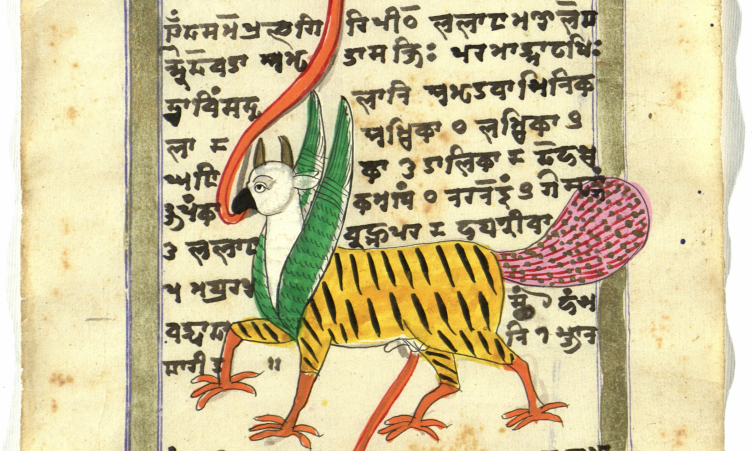
\includegraphics[width=1\textwidth]{pics/Wolpertinger.png}
\caption[The \textit{dehasvarūpa} of \textit{ajapāgāyatrī}]{The \textit{dehasvarūpa} of \textit{ajapāgāyatrī}. The image, reminiscent of a hippogriff, is part of an illustrated Sanskrit manuscript written in the Śāradā script. Preserved as a single large scroll under Acc. No. 1334 at the Oriental Institute in Srinagar (Kashmir), it is entitled \textit{Nāḍīcakra}. The manuscript contains a depiction of the yogic body’s \textit{cakra}s and \textit{nāḍī}s. The text surrounding the figure closely corresponds to the additional material found in manuscript \getsiglum{U2} of the \textit{Tattvayogabindu}. The manuscript reads (diplomatic transcription): \textit{oṃ daśame pūrṇagiripīṭhe lalāṭamaṇḍale candro devatā amṛtāśaktiḥ paramātmā ṛṣiḥ dvāviṃśaddalāni amṛtavāsinikalā 4: ambikā 1 lambikā 2 gha(ṃ)ṭkā 3 tālikā 4 dehasvarūpaṃ kākamukhaṃ 1 naranetraṃ 2 gośṛṅgaṃ 3 lalāṭabrahmapara 4 hayagrīvā 5 mayūramuśchaṃ 6 haṃsacārītani 7 sthāna.}}
	\phantomsection\label{fig_wolpertinger}
      \end{figure}

      \clearpage

  \begin{figure}[ht]
	\centering
  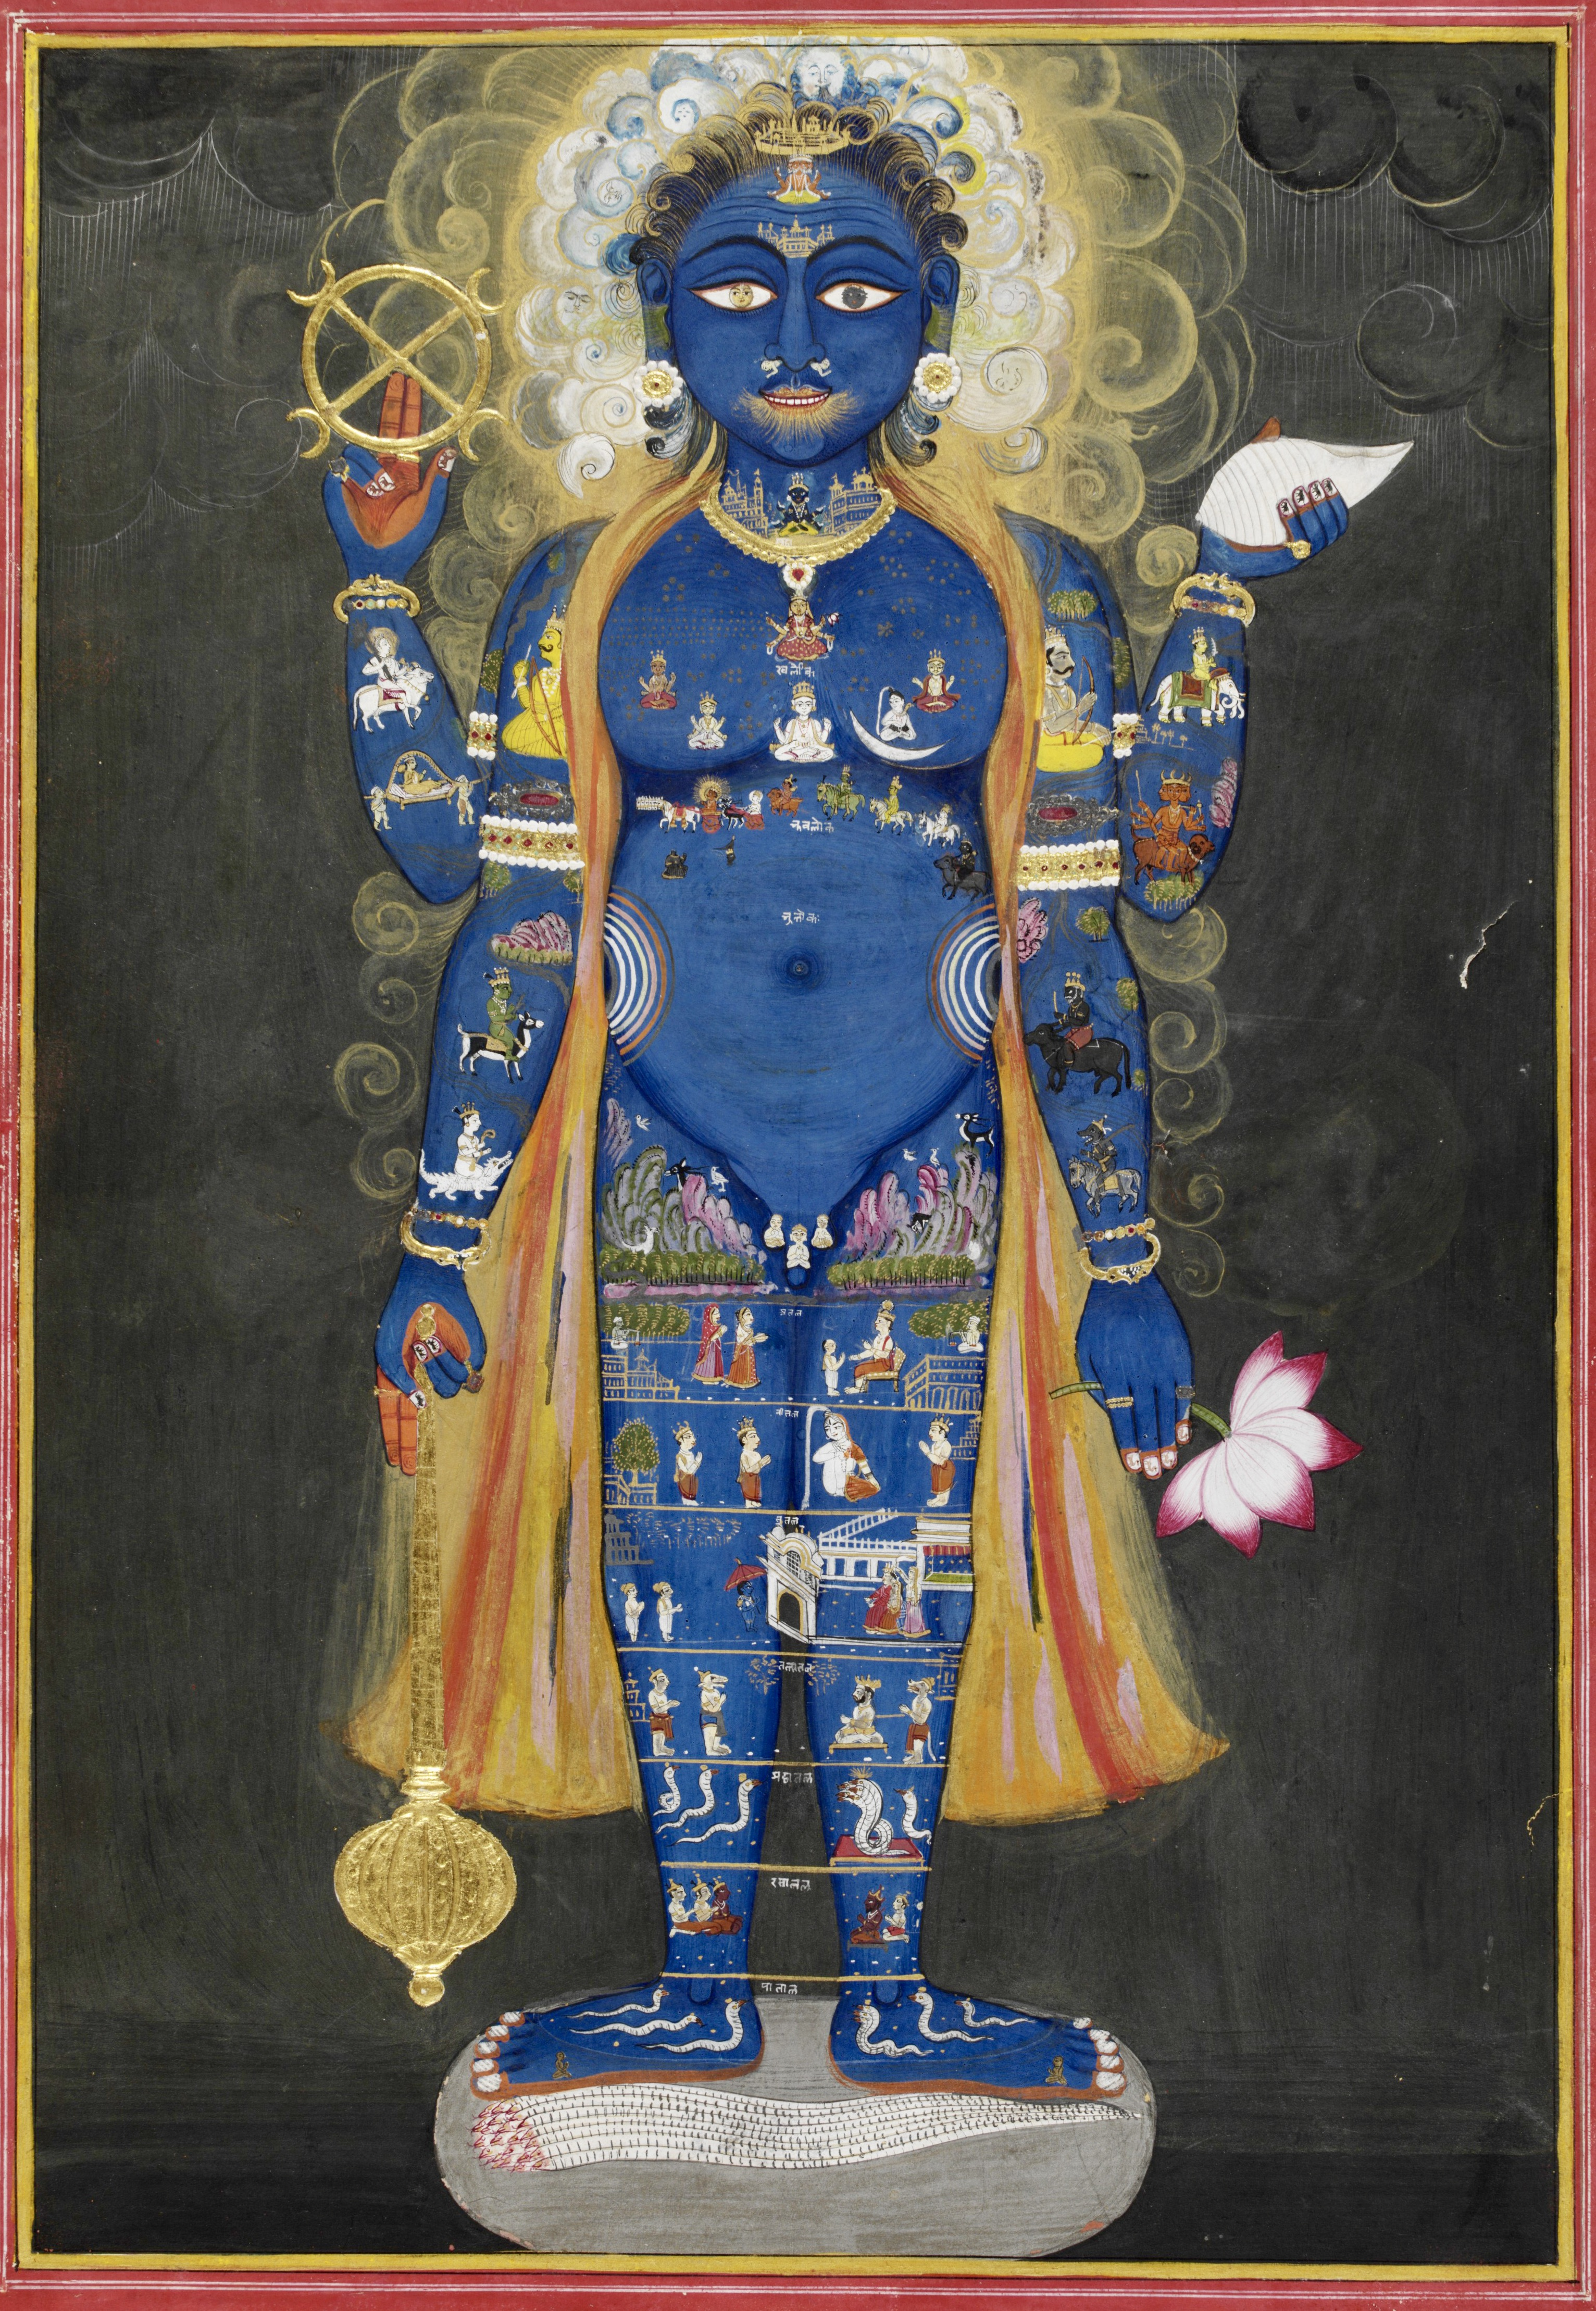
\includegraphics[width=1\textwidth]{pics/Vishnu_Vishvarupa_cropped.jpg}
	\caption{Viṣṇu Viśvarūpa, India, Rajasthan, Jaipur, ca. 1800–1820, Opaque watercolor and gold on paper, 38.5 × 28 cm, Victoria and Albert Museum, London, Given by Mrs. Gerald Clark.}
	\label{fig1}
      \end{figure}
\clearpage
  \begin{figure}[ht]
	\centering
  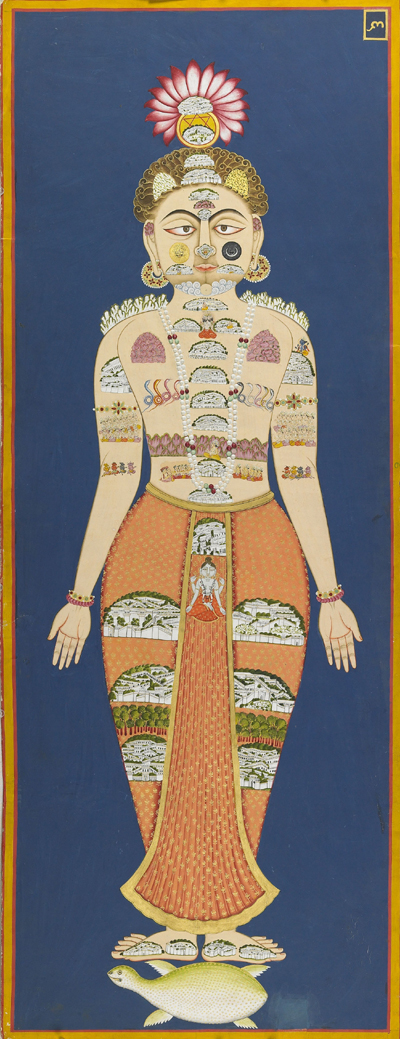
\includegraphics[width=0.5\textwidth]{pics/The_Equivalence_of_Self_and_Universe_(detail),_folio_6_from_the_Siddha_Siddhanta_Paddhati,_(Bulaki),_1824_(Samvat_1881);_122_x_46_cm._Mehrangarh_Museum_Trust..jpg}
	\caption{The Equivalence of Self and Universe (detail), folio 6 from the \textit{Siddhasiddhāntapaddhati} (Bulaki), India, Rajasthan, Jodhpur, 1824 (Samvat 1881), 122 x 46 cm, RJS 2378, Mehragarh Museum Trust.}
	\label{fig2}
      \end{figure}
      % \end{landscape}

      \newpage
      \cleardoublepage
\chapter{Bibliography}
 \label{sec:bibli}
\clearpage
\newpage 
\thispagestyle{empty}
\quad  \addtocounter{page}{-1}

\newrefcontext[sorting=tixel]
\printbibliography[heading=subbibintoc, title=Primary Sources, keyword=primary]

\newrefcontext[sorting=nyt]
\printbibliography[heading=subbibintoc, title=Secondary Literature, keyword=seclit]

\printbibliography[heading=subbibintoc, title=Catalogues, keyword=catalogues]

\printbibliography[heading=subbibintoc, title=Online Sources, keyword=onlinesource]

\end{document}


%%% Local Variables:
%%% mode: latex
%%% TeX-master: t
%%% End:
